\subsection{Studio della risoluzione temporale al variare dell'energia}

Una volta ultimata la calibrazione, si è voluto andare a stimare la risoluzione temporale dell'apparato al variare dell'energia depositata sui
rivelatori. Per farlo, si sono analizzati i dati con riferimento all'energia depositata all'interno dei rivelatori: quando la media dell'energia
depositata nei due rivelatori era sopra una certa soglia (o al di fuori della finestra prescelta) si è rimosso tale dato dal campione: ripetendo più
volte questo procedimento al variare della soglia e al variare della finestra è stato possibile stimare la risoluzione temporale. Tale
risoluzione è stata stimata andando a fare un'interpolazione gaussiana dei dati ottenuti in uscita dal TAC, selezionati come precedentemente descritto.
Dato che tale calcolo è stato fatto per molti intervalli di energia, non si riportano tutti i grafici creati singolarmente.
Nella tabella \ref{tab:cobalto_res} si possono leggere i risultati ottenuti. Per ottenere tali risultati l'interpolazione è stata fatta dopo aver calibrato i grafici e
considerando le calibrazioni come perfette (infatti per il conto della risoluzione non è necessaria una precisione così alta, e i risultati sono uguali a meno di ordini
superiori nell'errore)\\

%
\begin{table}
	\centering
	\begin{figure}[h] \centering\includegraphics[width=0.9\textwidth]{../../graphs/cobalto_risultati.tex}\caption{cobalto risultati}\label{gr:cobalto_risultati} \end{figure}

	\caption{La risoluzione temporale in funzione dell'energia}
	\label{tab:cobalto_res}
\end{table}
%
Nelle figure \ref{hist:bella_soglia} e \ref{hist:bella_intervalla} si sono riportate le gaussiane al variare rispettivamente della soglia e dell'intervallo utilizzato.
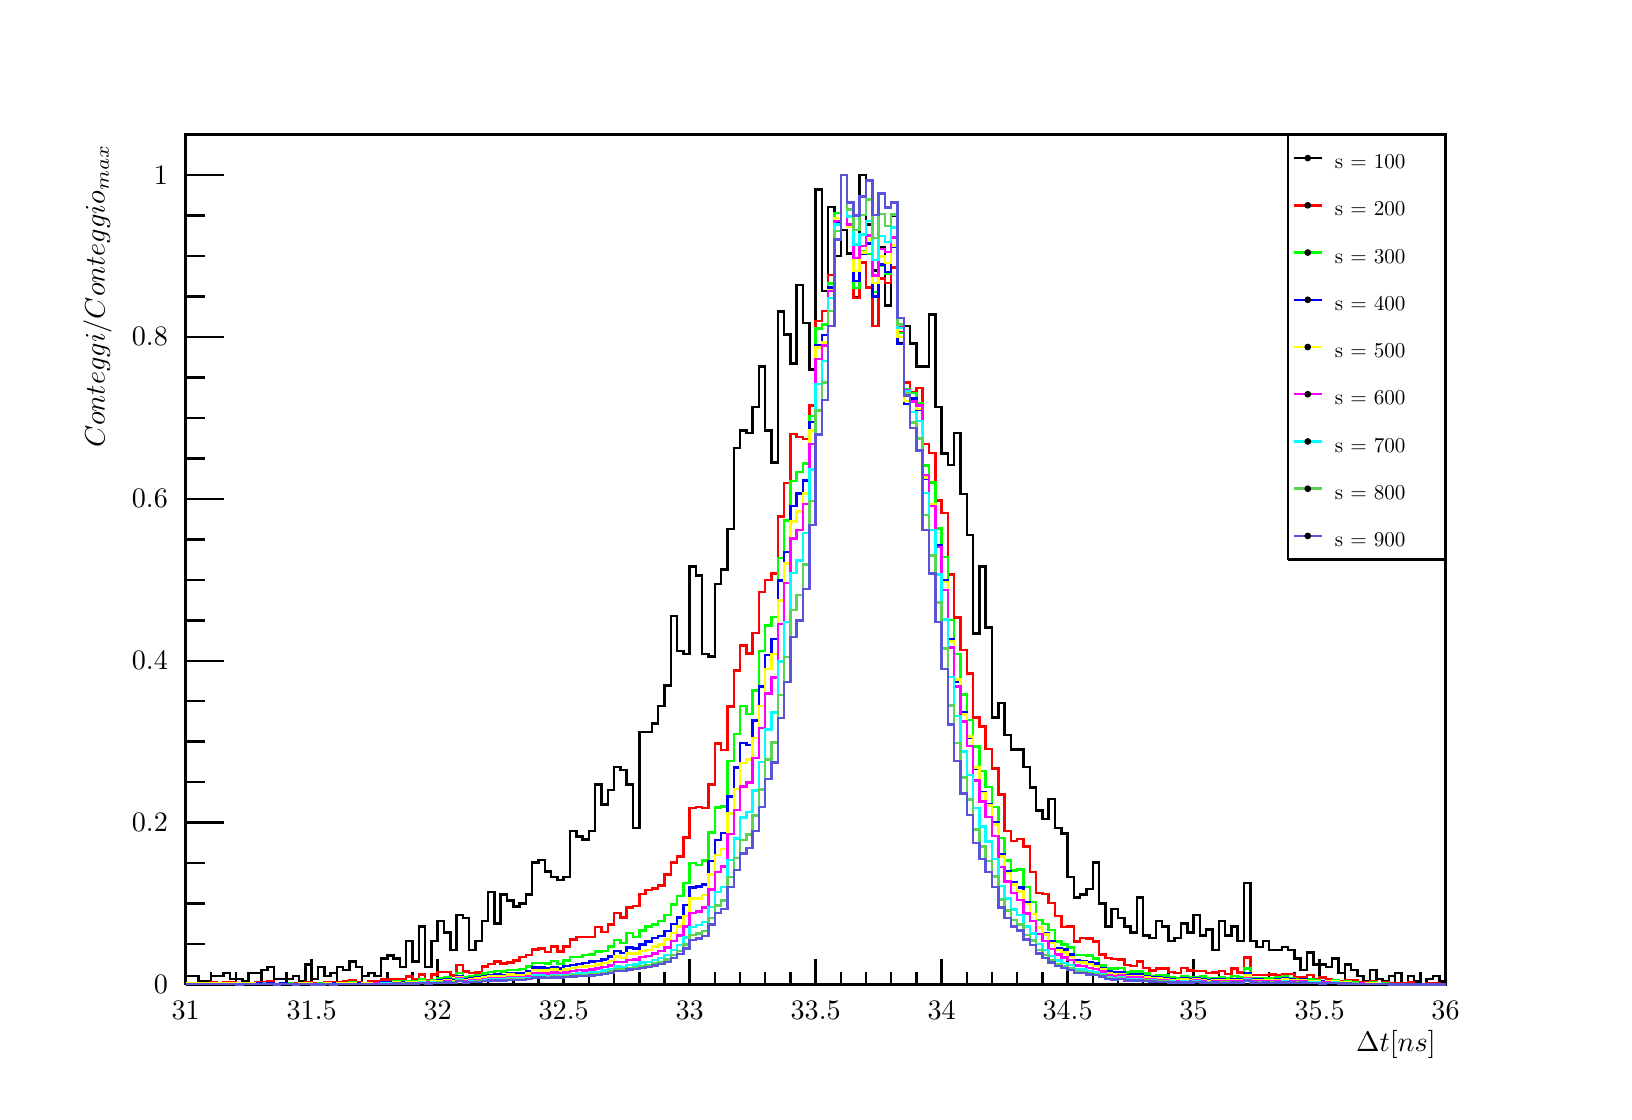
\begin{tikzpicture}
\pgfdeclareplotmark{cross} {
\pgfpathmoveto{\pgfpoint{-0.3\pgfplotmarksize}{\pgfplotmarksize}}
\pgfpathlineto{\pgfpoint{+0.3\pgfplotmarksize}{\pgfplotmarksize}}
\pgfpathlineto{\pgfpoint{+0.3\pgfplotmarksize}{0.3\pgfplotmarksize}}
\pgfpathlineto{\pgfpoint{+1\pgfplotmarksize}{0.3\pgfplotmarksize}}
\pgfpathlineto{\pgfpoint{+1\pgfplotmarksize}{-0.3\pgfplotmarksize}}
\pgfpathlineto{\pgfpoint{+0.3\pgfplotmarksize}{-0.3\pgfplotmarksize}}
\pgfpathlineto{\pgfpoint{+0.3\pgfplotmarksize}{-1.\pgfplotmarksize}}
\pgfpathlineto{\pgfpoint{-0.3\pgfplotmarksize}{-1.\pgfplotmarksize}}
\pgfpathlineto{\pgfpoint{-0.3\pgfplotmarksize}{-0.3\pgfplotmarksize}}
\pgfpathlineto{\pgfpoint{-1.\pgfplotmarksize}{-0.3\pgfplotmarksize}}
\pgfpathlineto{\pgfpoint{-1.\pgfplotmarksize}{0.3\pgfplotmarksize}}
\pgfpathlineto{\pgfpoint{-0.3\pgfplotmarksize}{0.3\pgfplotmarksize}}
\pgfpathclose
\pgfusepathqstroke
}
\pgfdeclareplotmark{cross*} {
\pgfpathmoveto{\pgfpoint{-0.3\pgfplotmarksize}{\pgfplotmarksize}}
\pgfpathlineto{\pgfpoint{+0.3\pgfplotmarksize}{\pgfplotmarksize}}
\pgfpathlineto{\pgfpoint{+0.3\pgfplotmarksize}{0.3\pgfplotmarksize}}
\pgfpathlineto{\pgfpoint{+1\pgfplotmarksize}{0.3\pgfplotmarksize}}
\pgfpathlineto{\pgfpoint{+1\pgfplotmarksize}{-0.3\pgfplotmarksize}}
\pgfpathlineto{\pgfpoint{+0.3\pgfplotmarksize}{-0.3\pgfplotmarksize}}
\pgfpathlineto{\pgfpoint{+0.3\pgfplotmarksize}{-1.\pgfplotmarksize}}
\pgfpathlineto{\pgfpoint{-0.3\pgfplotmarksize}{-1.\pgfplotmarksize}}
\pgfpathlineto{\pgfpoint{-0.3\pgfplotmarksize}{-0.3\pgfplotmarksize}}
\pgfpathlineto{\pgfpoint{-1.\pgfplotmarksize}{-0.3\pgfplotmarksize}}
\pgfpathlineto{\pgfpoint{-1.\pgfplotmarksize}{0.3\pgfplotmarksize}}
\pgfpathlineto{\pgfpoint{-0.3\pgfplotmarksize}{0.3\pgfplotmarksize}}
\pgfpathclose
\pgfusepathqfillstroke
}
\pgfdeclareplotmark{newstar} {
\pgfpathmoveto{\pgfqpoint{0pt}{\pgfplotmarksize}}
\pgfpathlineto{\pgfqpointpolar{44}{0.5\pgfplotmarksize}}
\pgfpathlineto{\pgfqpointpolar{18}{\pgfplotmarksize}}
\pgfpathlineto{\pgfqpointpolar{-20}{0.5\pgfplotmarksize}}
\pgfpathlineto{\pgfqpointpolar{-54}{\pgfplotmarksize}}
\pgfpathlineto{\pgfqpointpolar{-90}{0.5\pgfplotmarksize}}
\pgfpathlineto{\pgfqpointpolar{234}{\pgfplotmarksize}}
\pgfpathlineto{\pgfqpointpolar{198}{0.5\pgfplotmarksize}}
\pgfpathlineto{\pgfqpointpolar{162}{\pgfplotmarksize}}
\pgfpathlineto{\pgfqpointpolar{134}{0.5\pgfplotmarksize}}
\pgfpathclose
\pgfusepathqstroke
}
\pgfdeclareplotmark{newstar*} {
\pgfpathmoveto{\pgfqpoint{0pt}{\pgfplotmarksize}}
\pgfpathlineto{\pgfqpointpolar{44}{0.5\pgfplotmarksize}}
\pgfpathlineto{\pgfqpointpolar{18}{\pgfplotmarksize}}
\pgfpathlineto{\pgfqpointpolar{-20}{0.5\pgfplotmarksize}}
\pgfpathlineto{\pgfqpointpolar{-54}{\pgfplotmarksize}}
\pgfpathlineto{\pgfqpointpolar{-90}{0.5\pgfplotmarksize}}
\pgfpathlineto{\pgfqpointpolar{234}{\pgfplotmarksize}}
\pgfpathlineto{\pgfqpointpolar{198}{0.5\pgfplotmarksize}}
\pgfpathlineto{\pgfqpointpolar{162}{\pgfplotmarksize}}
\pgfpathlineto{\pgfqpointpolar{134}{0.5\pgfplotmarksize}}
\pgfpathclose
\pgfusepathqfillstroke
}
\definecolor{c}{rgb}{1,1,1};
\draw [color=c, fill=c] (0,0) rectangle (20,13.4957);
\draw [color=c, fill=c] (2,1.34957) rectangle (18,12.1461);
\definecolor{c}{rgb}{0,0,0};
\draw [c,line width=0.9] (2,1.34957) -- (2,12.1461) -- (18,12.1461) -- (18,1.34957) -- (2,1.34957);
\definecolor{c}{rgb}{1,1,1};
\draw [color=c, fill=c] (2,1.34957) rectangle (18,12.1461);
\definecolor{c}{rgb}{0,0,0};
\draw [c,line width=0.9] (2,1.34957) -- (2,12.1461) -- (18,12.1461) -- (18,1.34957) -- (2,1.34957);
\draw [c,line width=0.9] (2,1.46013) -- (2.08,1.46013) -- (2.08,1.46013) -- (2.16,1.46013) -- (2.16,1.38642) -- (2.24,1.38642) -- (2.24,1.38642) -- (2.32,1.38642) -- (2.32,1.46013) -- (2.4,1.46013) -- (2.4,1.46013) -- (2.48,1.46013) -- (2.48,1.49699)
 -- (2.56,1.49699) -- (2.56,1.42328) -- (2.64,1.42328) -- (2.64,1.42328) -- (2.72,1.42328) -- (2.72,1.38642) -- (2.8,1.38642) -- (2.8,1.49699) -- (2.88,1.49699) -- (2.88,1.49699) -- (2.96,1.49699) -- (2.96,1.53384) -- (3.04,1.53384) -- (3.04,1.5707)
 -- (3.12,1.5707) -- (3.12,1.42328) -- (3.2,1.42328) -- (3.2,1.42328) -- (3.28,1.42328) -- (3.28,1.42328) -- (3.36,1.42328) -- (3.36,1.46013) -- (3.44,1.46013) -- (3.44,1.38642) -- (3.52,1.38642) -- (3.52,1.60755) -- (3.6,1.60755) -- (3.6,1.42328) --
 (3.68,1.42328) -- (3.68,1.5707) -- (3.76,1.5707) -- (3.76,1.46013) -- (3.84,1.46013) -- (3.84,1.49699) -- (3.92,1.49699) -- (3.92,1.5707) -- (4,1.5707) -- (4,1.53384) -- (4.08,1.53384) -- (4.08,1.64441) -- (4.16,1.64441) -- (4.16,1.5707) --
 (4.24,1.5707) -- (4.24,1.46013) -- (4.32,1.46013) -- (4.32,1.49699) -- (4.4,1.49699) -- (4.4,1.46013) -- (4.48,1.46013) -- (4.48,1.68126) -- (4.56,1.68126) -- (4.56,1.71812) -- (4.64,1.71812) -- (4.64,1.68126) -- (4.72,1.68126) -- (4.72,1.5707) --
 (4.8,1.5707) -- (4.8,1.90239) -- (4.88,1.90239) -- (4.88,1.64441) -- (4.96,1.64441) -- (4.96,2.08666) -- (5.04,2.08666) -- (5.04,1.5707) -- (5.12,1.5707) -- (5.12,1.90239) -- (5.2,1.90239) -- (5.2,2.16037) -- (5.28,2.16037) -- (5.28,2.01295) --
 (5.36,2.01295) -- (5.36,1.79183) -- (5.44,1.79183) -- (5.44,2.23408) -- (5.52,2.23408) -- (5.52,2.19723) -- (5.6,2.19723) -- (5.6,1.79183) -- (5.68,1.79183) -- (5.68,1.90239) -- (5.76,1.90239) -- (5.76,2.16037) -- (5.84,2.16037) -- (5.84,2.52892) --
 (5.92,2.52892) -- (5.92,2.12352) -- (6,2.12352) -- (6,2.49206) -- (6.08,2.49206) -- (6.08,2.41835) -- (6.16,2.41835) -- (6.16,2.34465) -- (6.24,2.34465) -- (6.24,2.3815) -- (6.32,2.3815) -- (6.32,2.49206) -- (6.4,2.49206) -- (6.4,2.89746) --
 (6.48,2.89746) -- (6.48,2.93432) -- (6.56,2.93432) -- (6.56,2.7869) -- (6.64,2.7869) -- (6.64,2.71319) -- (6.72,2.71319) -- (6.72,2.67634) -- (6.8,2.67634) -- (6.8,2.71319) -- (6.88,2.71319) -- (6.88,3.30287) -- (6.96,3.30287) -- (6.96,3.22916) --
 (7.04,3.22916) -- (7.04,3.1923) -- (7.12,3.1923) -- (7.12,3.30287) -- (7.2,3.30287) -- (7.2,3.89254) -- (7.28,3.89254) -- (7.28,3.63456) -- (7.36,3.63456) -- (7.36,3.81883) -- (7.44,3.81883) -- (7.44,4.11367) -- (7.52,4.11367) -- (7.52,4.07681) --
 (7.6,4.07681) -- (7.6,3.89254) -- (7.68,3.89254) -- (7.68,3.33972) -- (7.76,3.33972) -- (7.76,4.55592) -- (7.84,4.55592) -- (7.84,4.55592) -- (7.92,4.55592) -- (7.92,4.66649) -- (8,4.66649) -- (8,4.88761) -- (8.08,4.88761) -- (8.08,5.1456) --
 (8.16,5.1456) -- (8.16,6.03011) -- (8.24,6.03011) -- (8.24,5.58785) -- (8.32,5.58785) -- (8.32,5.551) -- (8.4,5.551) -- (8.4,6.65664) -- (8.48,6.65664) -- (8.48,6.54607) -- (8.56,6.54607) -- (8.56,5.551) -- (8.64,5.551) -- (8.64,5.51414) --
 (8.72,5.51414) -- (8.72,6.43551) -- (8.8,6.43551) -- (8.8,6.61978) -- (8.88,6.61978) -- (8.88,7.13575) -- (8.96,7.13575) -- (8.96,8.16768) -- (9.04,8.16768) -- (9.04,8.3888) -- (9.12,8.3888) -- (9.12,8.35195) -- (9.2,8.35195) -- (9.2,8.68364) --
 (9.28,8.68364) -- (9.28,9.1996) -- (9.36,9.1996) -- (9.36,8.3888) -- (9.44,8.3888) -- (9.44,7.9834) -- (9.52,7.9834) -- (9.52,9.89984) -- (9.6,9.89984) -- (9.6,9.60501) -- (9.68,9.60501) -- (9.68,9.23646) -- (9.76,9.23646) -- (9.76,10.2315) --
 (9.84,10.2315) -- (9.84,9.75242) -- (9.92,9.75242) -- (9.92,9.16275) -- (10,9.16275) -- (10,11.4477) -- (10.08,11.4477) -- (10.08,10.1578) -- (10.16,10.1578) -- (10.16,11.2266) -- (10.24,11.2266) -- (10.24,10.6001) -- (10.32,10.6001) --
 (10.32,10.9318) -- (10.4,10.9318) -- (10.4,10.6369) -- (10.48,10.6369) -- (10.48,10.0841) -- (10.56,10.0841) -- (10.56,11.632) -- (10.64,11.632) -- (10.64,11.0055) -- (10.72,11.0055) -- (10.72,10.4158) -- (10.8,10.4158) -- (10.8,10.7106) --
 (10.88,10.7106) -- (10.88,9.97355) -- (10.96,9.97355) -- (10.96,11.116) -- (11.04,11.116) -- (11.04,9.49444) -- (11.12,9.49444) -- (11.12,9.71557) -- (11.2,9.71557) -- (11.2,9.49444) -- (11.28,9.49444) -- (11.28,9.1996) -- (11.36,9.1996) --
 (11.36,9.1996) -- (11.44,9.1996) -- (11.44,9.86299) -- (11.52,9.86299) -- (11.52,8.68364) -- (11.6,8.68364) -- (11.6,8.09397) -- (11.68,8.09397) -- (11.68,7.94655) -- (11.76,7.94655) -- (11.76,8.35195) -- (11.84,8.35195) -- (11.84,7.578) --
 (11.92,7.578) -- (11.92,7.06204) -- (12,7.06204) -- (12,5.80898) -- (12.08,5.80898) -- (12.08,6.65664) -- (12.16,6.65664) -- (12.16,5.88269) -- (12.24,5.88269) -- (12.24,4.7402) -- (12.32,4.7402) -- (12.32,4.92447) -- (12.4,4.92447) --
 (12.4,4.51907) -- (12.48,4.51907) -- (12.48,4.33479) -- (12.56,4.33479) -- (12.56,4.33479) -- (12.64,4.33479) -- (12.64,4.11367) -- (12.72,4.11367) -- (12.72,3.85568) -- (12.8,3.85568) -- (12.8,3.56085) -- (12.88,3.56085) -- (12.88,3.45028) --
 (12.96,3.45028) -- (12.96,3.70827) -- (13.04,3.70827) -- (13.04,3.33972) -- (13.12,3.33972) -- (13.12,3.26601) -- (13.2,3.26601) -- (13.2,2.71319) -- (13.28,2.71319) -- (13.28,2.45521) -- (13.36,2.45521) -- (13.36,2.49206) -- (13.44,2.49206) --
 (13.44,2.56577) -- (13.52,2.56577) -- (13.52,2.89746) -- (13.6,2.89746) -- (13.6,2.3815) -- (13.68,2.3815) -- (13.68,2.08666) -- (13.76,2.08666) -- (13.76,2.30779) -- (13.84,2.30779) -- (13.84,2.19723) -- (13.92,2.19723) -- (13.92,2.08666) --
 (14,2.08666) -- (14,2.01295) -- (14.08,2.01295) -- (14.08,2.45521) -- (14.16,2.45521) -- (14.16,1.9761) -- (14.24,1.9761) -- (14.24,1.93924) -- (14.32,1.93924) -- (14.32,2.16037) -- (14.4,2.16037) -- (14.4,2.08666) -- (14.48,2.08666) --
 (14.48,1.90239) -- (14.56,1.90239) -- (14.56,1.93924) -- (14.64,1.93924) -- (14.64,2.12352) -- (14.72,2.12352) -- (14.72,2.01295) -- (14.8,2.01295) -- (14.8,2.23408) -- (14.88,2.23408) -- (14.88,1.9761) -- (14.96,1.9761) -- (14.96,2.04981) --
 (15.04,2.04981) -- (15.04,1.79183) -- (15.12,1.79183) -- (15.12,2.16037) -- (15.2,2.16037) -- (15.2,1.9761) -- (15.28,1.9761) -- (15.28,2.08666) -- (15.36,2.08666) -- (15.36,1.90239) -- (15.44,1.90239) -- (15.44,2.63948) -- (15.52,2.63948) --
 (15.52,1.90239) -- (15.6,1.90239) -- (15.6,1.82868) -- (15.68,1.82868) -- (15.68,1.90239) -- (15.76,1.90239) -- (15.76,1.79183) -- (15.84,1.79183) -- (15.84,1.79183) -- (15.92,1.79183) -- (15.92,1.82868) -- (16,1.82868) -- (16,1.79183) --
 (16.08,1.79183) -- (16.08,1.68126) -- (16.16,1.68126) -- (16.16,1.53384) -- (16.24,1.53384) -- (16.24,1.75497) -- (16.32,1.75497) -- (16.32,1.60755) -- (16.4,1.60755) -- (16.4,1.60755) -- (16.48,1.60755) -- (16.48,1.5707) -- (16.56,1.5707) --
 (16.56,1.68126) -- (16.64,1.68126) -- (16.64,1.49699) -- (16.72,1.49699) -- (16.72,1.60755) -- (16.8,1.60755) -- (16.8,1.53384) -- (16.88,1.53384) -- (16.88,1.46013) -- (16.96,1.46013) -- (16.96,1.38642) -- (17.04,1.38642) -- (17.04,1.53384) --
 (17.12,1.53384) -- (17.12,1.42328) -- (17.2,1.42328) -- (17.2,1.38642) -- (17.28,1.38642) -- (17.28,1.46013) -- (17.36,1.46013) -- (17.36,1.49699) -- (17.44,1.49699) -- (17.44,1.34957) -- (17.52,1.34957) -- (17.52,1.46013) -- (17.6,1.46013) --
 (17.6,1.38642) -- (17.68,1.38642) -- (17.68,1.34957) -- (17.76,1.34957) -- (17.76,1.42328) -- (17.84,1.42328) -- (17.84,1.46013) -- (17.92,1.46013) -- (17.92,1.38642) -- (18,1.38642);
\draw [c,line width=0.9] (2,1.34957) -- (18,1.34957);
\draw [anchor= east] (18,0.593811) node[scale=1.01821, color=c, rotate=0]{$\Delta t [ns]$};
\draw [c,line width=0.9] (2,1.67347) -- (2,1.34957);
\draw [c,line width=0.9] (2.32,1.51152) -- (2.32,1.34957);
\draw [c,line width=0.9] (2.64,1.51152) -- (2.64,1.34957);
\draw [c,line width=0.9] (2.96,1.51152) -- (2.96,1.34957);
\draw [c,line width=0.9] (3.28,1.51152) -- (3.28,1.34957);
\draw [c,line width=0.9] (3.6,1.67347) -- (3.6,1.34957);
\draw [c,line width=0.9] (3.92,1.51152) -- (3.92,1.34957);
\draw [c,line width=0.9] (4.24,1.51152) -- (4.24,1.34957);
\draw [c,line width=0.9] (4.56,1.51152) -- (4.56,1.34957);
\draw [c,line width=0.9] (4.88,1.51152) -- (4.88,1.34957);
\draw [c,line width=0.9] (5.2,1.67347) -- (5.2,1.34957);
\draw [c,line width=0.9] (5.52,1.51152) -- (5.52,1.34957);
\draw [c,line width=0.9] (5.84,1.51152) -- (5.84,1.34957);
\draw [c,line width=0.9] (6.16,1.51152) -- (6.16,1.34957);
\draw [c,line width=0.9] (6.48,1.51152) -- (6.48,1.34957);
\draw [c,line width=0.9] (6.8,1.67347) -- (6.8,1.34957);
\draw [c,line width=0.9] (7.12,1.51152) -- (7.12,1.34957);
\draw [c,line width=0.9] (7.44,1.51152) -- (7.44,1.34957);
\draw [c,line width=0.9] (7.76,1.51152) -- (7.76,1.34957);
\draw [c,line width=0.9] (8.08,1.51152) -- (8.08,1.34957);
\draw [c,line width=0.9] (8.4,1.67347) -- (8.4,1.34957);
\draw [c,line width=0.9] (8.72,1.51152) -- (8.72,1.34957);
\draw [c,line width=0.9] (9.04,1.51152) -- (9.04,1.34957);
\draw [c,line width=0.9] (9.36,1.51152) -- (9.36,1.34957);
\draw [c,line width=0.9] (9.68,1.51152) -- (9.68,1.34957);
\draw [c,line width=0.9] (10,1.67347) -- (10,1.34957);
\draw [c,line width=0.9] (10.32,1.51152) -- (10.32,1.34957);
\draw [c,line width=0.9] (10.64,1.51152) -- (10.64,1.34957);
\draw [c,line width=0.9] (10.96,1.51152) -- (10.96,1.34957);
\draw [c,line width=0.9] (11.28,1.51152) -- (11.28,1.34957);
\draw [c,line width=0.9] (11.6,1.67347) -- (11.6,1.34957);
\draw [c,line width=0.9] (11.92,1.51152) -- (11.92,1.34957);
\draw [c,line width=0.9] (12.24,1.51152) -- (12.24,1.34957);
\draw [c,line width=0.9] (12.56,1.51152) -- (12.56,1.34957);
\draw [c,line width=0.9] (12.88,1.51152) -- (12.88,1.34957);
\draw [c,line width=0.9] (13.2,1.67347) -- (13.2,1.34957);
\draw [c,line width=0.9] (13.52,1.51152) -- (13.52,1.34957);
\draw [c,line width=0.9] (13.84,1.51152) -- (13.84,1.34957);
\draw [c,line width=0.9] (14.16,1.51152) -- (14.16,1.34957);
\draw [c,line width=0.9] (14.48,1.51152) -- (14.48,1.34957);
\draw [c,line width=0.9] (14.8,1.67347) -- (14.8,1.34957);
\draw [c,line width=0.9] (15.12,1.51152) -- (15.12,1.34957);
\draw [c,line width=0.9] (15.44,1.51152) -- (15.44,1.34957);
\draw [c,line width=0.9] (15.76,1.51152) -- (15.76,1.34957);
\draw [c,line width=0.9] (16.08,1.51152) -- (16.08,1.34957);
\draw [c,line width=0.9] (16.4,1.67347) -- (16.4,1.34957);
\draw [c,line width=0.9] (16.72,1.51152) -- (16.72,1.34957);
\draw [c,line width=0.9] (17.04,1.51152) -- (17.04,1.34957);
\draw [c,line width=0.9] (17.36,1.51152) -- (17.36,1.34957);
\draw [c,line width=0.9] (17.68,1.51152) -- (17.68,1.34957);
\draw [c,line width=0.9] (18,1.67347) -- (18,1.34957);
\draw [anchor=base] (2,0.904212) node[scale=1.01821, color=c, rotate=0]{31};
\draw [anchor=base] (3.6,0.904212) node[scale=1.01821, color=c, rotate=0]{31.5};
\draw [anchor=base] (5.2,0.904212) node[scale=1.01821, color=c, rotate=0]{32};
\draw [anchor=base] (6.8,0.904212) node[scale=1.01821, color=c, rotate=0]{32.5};
\draw [anchor=base] (8.4,0.904212) node[scale=1.01821, color=c, rotate=0]{33};
\draw [anchor=base] (10,0.904212) node[scale=1.01821, color=c, rotate=0]{33.5};
\draw [anchor=base] (11.6,0.904212) node[scale=1.01821, color=c, rotate=0]{34};
\draw [anchor=base] (13.2,0.904212) node[scale=1.01821, color=c, rotate=0]{34.5};
\draw [anchor=base] (14.8,0.904212) node[scale=1.01821, color=c, rotate=0]{35};
\draw [anchor=base] (16.4,0.904212) node[scale=1.01821, color=c, rotate=0]{35.5};
\draw [anchor=base] (18,0.904212) node[scale=1.01821, color=c, rotate=0]{36};
\draw [c,line width=0.9] (2,1.34957) -- (2,12.1461);
\draw [anchor= east] (0.88,12.1461) node[scale=1.01821, color=c, rotate=90]{$Conteggi/Conteggio_{max}$};
\draw [c,line width=0.9] (2.48,1.34957) -- (2,1.34957);
\draw [c,line width=0.9] (2.24,1.86369) -- (2,1.86369);
\draw [c,line width=0.9] (2.24,2.37781) -- (2,2.37781);
\draw [c,line width=0.9] (2.24,2.89194) -- (2,2.89194);
\draw [c,line width=0.9] (2.48,3.40606) -- (2,3.40606);
\draw [c,line width=0.9] (2.24,3.92018) -- (2,3.92018);
\draw [c,line width=0.9] (2.24,4.4343) -- (2,4.4343);
\draw [c,line width=0.9] (2.24,4.94842) -- (2,4.94842);
\draw [c,line width=0.9] (2.48,5.46255) -- (2,5.46255);
\draw [c,line width=0.9] (2.24,5.97667) -- (2,5.97667);
\draw [c,line width=0.9] (2.24,6.49079) -- (2,6.49079);
\draw [c,line width=0.9] (2.24,7.00491) -- (2,7.00491);
\draw [c,line width=0.9] (2.48,7.51903) -- (2,7.51903);
\draw [c,line width=0.9] (2.24,8.03316) -- (2,8.03316);
\draw [c,line width=0.9] (2.24,8.54728) -- (2,8.54728);
\draw [c,line width=0.9] (2.24,9.0614) -- (2,9.0614);
\draw [c,line width=0.9] (2.48,9.57552) -- (2,9.57552);
\draw [c,line width=0.9] (2.24,10.0896) -- (2,10.0896);
\draw [c,line width=0.9] (2.24,10.6038) -- (2,10.6038);
\draw [c,line width=0.9] (2.24,11.1179) -- (2,11.1179);
\draw [c,line width=0.9] (2.48,11.632) -- (2,11.632);
\draw [c,line width=0.9] (2.48,11.632) -- (2,11.632);
\draw [anchor= east] (1.9,1.34957) node[scale=1.01821, color=c, rotate=0]{0};
\draw [anchor= east] (1.9,3.40606) node[scale=1.01821, color=c, rotate=0]{0.2};
\draw [anchor= east] (1.9,5.46255) node[scale=1.01821, color=c, rotate=0]{0.4};
\draw [anchor= east] (1.9,7.51903) node[scale=1.01821, color=c, rotate=0]{0.6};
\draw [anchor= east] (1.9,9.57552) node[scale=1.01821, color=c, rotate=0]{0.8};
\draw [anchor= east] (1.9,11.632) node[scale=1.01821, color=c, rotate=0]{1};
\definecolor{c}{rgb}{1,0,0};
\draw [c,line width=0.9] (2,1.37069) -- (2.08,1.37069) -- (2.08,1.36717) -- (2.16,1.36717) -- (2.16,1.36717) -- (2.24,1.36717) -- (2.24,1.36013) -- (2.32,1.36013) -- (2.32,1.38125) -- (2.4,1.38125) -- (2.4,1.36717) -- (2.48,1.36717) -- (2.48,1.38477)
 -- (2.56,1.38477) -- (2.56,1.38477) -- (2.64,1.38477) -- (2.64,1.36013) -- (2.72,1.36013) -- (2.72,1.37069) -- (2.8,1.37069) -- (2.8,1.36717) -- (2.88,1.36717) -- (2.88,1.38477) -- (2.96,1.38477) -- (2.96,1.37773) -- (3.04,1.37773) -- (3.04,1.39181)
 -- (3.12,1.39181) -- (3.12,1.36013) -- (3.2,1.36013) -- (3.2,1.37069) -- (3.28,1.37069) -- (3.28,1.37069) -- (3.36,1.37069) -- (3.36,1.36717) -- (3.44,1.36717) -- (3.44,1.36365) -- (3.52,1.36365) -- (3.52,1.38477) -- (3.6,1.38477) -- (3.6,1.37069)
 -- (3.68,1.37069) -- (3.68,1.37069) -- (3.76,1.37069) -- (3.76,1.37421) -- (3.84,1.37421) -- (3.84,1.37773) -- (3.92,1.37773) -- (3.92,1.37773) -- (4,1.37773) -- (4,1.39181) -- (4.08,1.39181) -- (4.08,1.40237) -- (4.16,1.40237) -- (4.16,1.37773) --
 (4.24,1.37773) -- (4.24,1.36013) -- (4.32,1.36013) -- (4.32,1.39181) -- (4.4,1.39181) -- (4.4,1.39181) -- (4.48,1.39181) -- (4.48,1.41293) -- (4.56,1.41293) -- (4.56,1.41293) -- (4.64,1.41293) -- (4.64,1.42349) -- (4.72,1.42349) -- (4.72,1.41293) --
 (4.8,1.41293) -- (4.8,1.45166) -- (4.88,1.45166) -- (4.88,1.42349) -- (4.96,1.42349) -- (4.96,1.4763) -- (5.04,1.4763) -- (5.04,1.40589) -- (5.12,1.40589) -- (5.12,1.4763) -- (5.2,1.4763) -- (5.2,1.5115) -- (5.28,1.5115) -- (5.28,1.5115) --
 (5.36,1.5115) -- (5.36,1.46222) -- (5.44,1.46222) -- (5.44,1.5995) -- (5.52,1.5995) -- (5.52,1.51854) -- (5.6,1.51854) -- (5.6,1.4939) -- (5.68,1.4939) -- (5.68,1.50446) -- (5.76,1.50446) -- (5.76,1.57838) -- (5.84,1.57838) -- (5.84,1.61358) --
 (5.92,1.61358) -- (5.92,1.64174) -- (6,1.64174) -- (6,1.6171) -- (6.08,1.6171) -- (6.08,1.62766) -- (6.16,1.62766) -- (6.16,1.65583) -- (6.24,1.65583) -- (6.24,1.70159) -- (6.32,1.70159) -- (6.32,1.72623) -- (6.4,1.72623) -- (6.4,1.79311) --
 (6.48,1.79311) -- (6.48,1.81071) -- (6.56,1.81071) -- (6.56,1.76495) -- (6.64,1.76495) -- (6.64,1.83535) -- (6.72,1.83535) -- (6.72,1.77199) -- (6.8,1.77199) -- (6.8,1.83535) -- (6.88,1.83535) -- (6.88,1.92336) -- (6.96,1.92336) -- (6.96,1.95504) --
 (7.04,1.95504) -- (7.04,1.95504) -- (7.12,1.95504) -- (7.12,1.95504) -- (7.2,1.95504) -- (7.2,2.07825) -- (7.28,2.07825) -- (7.28,2.01488) -- (7.36,2.01488) -- (7.36,2.11345) -- (7.44,2.11345) -- (7.44,2.2613) -- (7.52,2.2613) -- (7.52,2.20497) --
 (7.6,2.20497) -- (7.6,2.32818) -- (7.68,2.32818) -- (7.68,2.3493) -- (7.76,2.3493) -- (7.76,2.50067) -- (7.84,2.50067) -- (7.84,2.54995) -- (7.92,2.54995) -- (7.92,2.57107) -- (8,2.57107) -- (8,2.60627) -- (8.08,2.60627) -- (8.08,2.7506) --
 (8.16,2.7506) -- (8.16,2.89845) -- (8.24,2.89845) -- (8.24,2.97941) -- (8.32,2.97941) -- (8.32,3.21526) -- (8.4,3.21526) -- (8.4,3.59544) -- (8.48,3.59544) -- (8.48,3.60248) -- (8.56,3.60248) -- (8.56,3.59192) -- (8.64,3.59192) -- (8.64,3.89114) --
 (8.72,3.89114) -- (8.72,4.4086) -- (8.8,4.4086) -- (8.8,4.32764) -- (8.88,4.32764) -- (8.88,4.88383) -- (8.96,4.88383) -- (8.96,5.34145) -- (9.04,5.34145) -- (9.04,5.65475) -- (9.12,5.65475) -- (9.12,5.55266) -- (9.2,5.55266) -- (9.2,5.81668) --
 (9.28,5.81668) -- (9.28,6.33414) -- (9.36,6.33414) -- (9.36,6.48903) -- (9.44,6.48903) -- (9.44,6.57351) -- (9.52,6.57351) -- (9.52,7.29515) -- (9.6,7.29515) -- (9.6,7.72109) -- (9.68,7.72109) -- (9.68,8.34064) -- (9.76,8.34064) -- (9.76,8.30192) --
 (9.84,8.30192) -- (9.84,8.2808) -- (9.92,8.2808) -- (9.92,8.70674) -- (10,8.70674) -- (10,9.7804) -- (10.08,9.7804) -- (10.08,9.9036) -- (10.16,9.9036) -- (10.16,10.3647) -- (10.24,10.3647) -- (10.24,11.0265) -- (10.32,11.0265) -- (10.32,11.632) --
 (10.4,11.632) -- (10.4,10.9702) -- (10.48,10.9702) -- (10.48,10.0726) -- (10.56,10.0726) -- (10.56,10.5232) -- (10.64,10.5232) -- (10.64,10.2028) -- (10.72,10.2028) -- (10.72,9.71703) -- (10.8,9.71703) -- (10.8,10.3155) -- (10.88,10.3155) --
 (10.88,10.2627) -- (10.96,10.2627) -- (10.96,10.4563) -- (11.04,10.4563) -- (11.04,9.62903) -- (11.12,9.62903) -- (11.12,8.99892) -- (11.2,8.99892) -- (11.2,8.86867) -- (11.28,8.86867) -- (11.28,8.92499) -- (11.36,8.92499) -- (11.36,8.21744) --
 (11.44,8.21744) -- (11.44,8.10127) -- (11.52,8.10127) -- (11.52,7.49932) -- (11.6,7.49932) -- (11.6,7.34091) -- (11.68,7.34091) -- (11.68,6.55943) -- (11.76,6.55943) -- (11.76,6.01029) -- (11.84,6.01029) -- (11.84,5.60194) -- (11.92,5.60194) --
 (11.92,5.29921) -- (12,5.29921) -- (12,4.74302) -- (12.08,4.74302) -- (12.08,4.62686) -- (12.16,4.62686) -- (12.16,4.34172) -- (12.24,4.34172) -- (12.24,4.09179) -- (12.32,4.09179) -- (12.32,3.76441) -- (12.4,3.76441) -- (12.4,3.30327) --
 (12.48,3.30327) -- (12.48,3.17654) -- (12.56,3.17654) -- (12.56,3.20118) -- (12.64,3.20118) -- (12.64,3.10262) -- (12.72,3.10262) -- (12.72,2.77876) -- (12.8,2.77876) -- (12.8,2.51123) -- (12.88,2.51123) -- (12.88,2.50067) -- (12.96,2.50067) --
 (12.96,2.3845) -- (13.04,2.3845) -- (13.04,2.21905) -- (13.12,2.21905) -- (13.12,2.07825) -- (13.2,2.07825) -- (13.2,2.08529) -- (13.28,2.08529) -- (13.28,1.89872) -- (13.36,1.89872) -- (13.36,1.94448) -- (13.44,1.94448) -- (13.44,1.93392) --
 (13.52,1.93392) -- (13.52,1.8952) -- (13.6,1.8952) -- (13.6,1.72975) -- (13.68,1.72975) -- (13.68,1.68751) -- (13.76,1.68751) -- (13.76,1.67695) -- (13.84,1.67695) -- (13.84,1.66991) -- (13.92,1.66991) -- (13.92,1.59598) -- (14,1.59598) --
 (14,1.58894) -- (14.08,1.58894) -- (14.08,1.64174) -- (14.16,1.64174) -- (14.16,1.56078) -- (14.24,1.56078) -- (14.24,1.5291) -- (14.32,1.5291) -- (14.32,1.55726) -- (14.4,1.55726) -- (14.4,1.55374) -- (14.48,1.55374) -- (14.48,1.50798) --
 (14.56,1.50798) -- (14.56,1.4939) -- (14.64,1.4939) -- (14.64,1.56078) -- (14.72,1.56078) -- (14.72,1.5291) -- (14.8,1.5291) -- (14.8,1.52206) -- (14.88,1.52206) -- (14.88,1.52558) -- (14.96,1.52558) -- (14.96,1.49742) -- (15.04,1.49742) --
 (15.04,1.50446) -- (15.12,1.50446) -- (15.12,1.52558) -- (15.2,1.52558) -- (15.2,1.48686) -- (15.28,1.48686) -- (15.28,1.55374) -- (15.36,1.55374) -- (15.36,1.50094) -- (15.44,1.50094) -- (15.44,1.69103) -- (15.52,1.69103) -- (15.52,1.47278) --
 (15.6,1.47278) -- (15.6,1.47278) -- (15.68,1.47278) -- (15.68,1.46926) -- (15.76,1.46926) -- (15.76,1.47982) -- (15.84,1.47982) -- (15.84,1.46926) -- (15.92,1.46926) -- (15.92,1.4763) -- (16,1.4763) -- (16,1.48686) -- (16.08,1.48686) --
 (16.08,1.44814) -- (16.16,1.44814) -- (16.16,1.44814) -- (16.24,1.44814) -- (16.24,1.47278) -- (16.32,1.47278) -- (16.32,1.41645) -- (16.4,1.41645) -- (16.4,1.43757) -- (16.48,1.43757) -- (16.48,1.41645) -- (16.56,1.41645) -- (16.56,1.40941) --
 (16.64,1.40941) -- (16.64,1.39181) -- (16.72,1.39181) -- (16.72,1.40237) -- (16.8,1.40237) -- (16.8,1.40237) -- (16.88,1.40237) -- (16.88,1.37773) -- (16.96,1.37773) -- (16.96,1.38125) -- (17.04,1.38125) -- (17.04,1.38829) -- (17.12,1.38829) --
 (17.12,1.36013) -- (17.2,1.36013) -- (17.2,1.37421) -- (17.28,1.37421) -- (17.28,1.37069) -- (17.36,1.37069) -- (17.36,1.37069) -- (17.44,1.37069) -- (17.44,1.36365) -- (17.52,1.36365) -- (17.52,1.37421) -- (17.6,1.37421) -- (17.6,1.35661) --
 (17.68,1.35661) -- (17.68,1.35661) -- (17.76,1.35661) -- (17.76,1.36717) -- (17.84,1.36717) -- (17.84,1.36365) -- (17.92,1.36365) -- (17.92,1.35309) -- (18,1.35309);
\definecolor{c}{rgb}{0,1,0};
\draw [c,line width=0.9] (2,1.36884) -- (2.08,1.36884) -- (2.08,1.36196) -- (2.16,1.36196) -- (2.16,1.35783) -- (2.24,1.35783) -- (2.24,1.35645) -- (2.32,1.35645) -- (2.32,1.36746) -- (2.4,1.36746) -- (2.4,1.36196) -- (2.48,1.36196) -- (2.48,1.37159)
 -- (2.56,1.37159) -- (2.56,1.36746) -- (2.64,1.36746) -- (2.64,1.35783) -- (2.72,1.35783) -- (2.72,1.36196) -- (2.8,1.36196) -- (2.8,1.36334) -- (2.88,1.36334) -- (2.88,1.36334) -- (2.96,1.36334) -- (2.96,1.36334) -- (3.04,1.36334) -- (3.04,1.36746)
 -- (3.12,1.36746) -- (3.12,1.35645) -- (3.2,1.35645) -- (3.2,1.36471) -- (3.28,1.36471) -- (3.28,1.36334) -- (3.36,1.36334) -- (3.36,1.35783) -- (3.44,1.35783) -- (3.44,1.36196) -- (3.52,1.36196) -- (3.52,1.36884) -- (3.6,1.36884) -- (3.6,1.36058)
 -- (3.68,1.36058) -- (3.68,1.36196) -- (3.76,1.36196) -- (3.76,1.36334) -- (3.84,1.36334) -- (3.84,1.36471) -- (3.92,1.36471) -- (3.92,1.36884) -- (4,1.36884) -- (4,1.36884) -- (4.08,1.36884) -- (4.08,1.3771) -- (4.16,1.3771) -- (4.16,1.36196) --
 (4.24,1.36196) -- (4.24,1.36058) -- (4.32,1.36058) -- (4.32,1.37022) -- (4.4,1.37022) -- (4.4,1.37159) -- (4.48,1.37159) -- (4.48,1.38536) -- (4.56,1.38536) -- (4.56,1.38123) -- (4.64,1.38123) -- (4.64,1.38949) -- (4.72,1.38949) -- (4.72,1.38674) --
 (4.8,1.38674) -- (4.8,1.39499) -- (4.88,1.39499) -- (4.88,1.39499) -- (4.96,1.39499) -- (4.96,1.41702) -- (5.04,1.41702) -- (5.04,1.38674) -- (5.12,1.38674) -- (5.12,1.41014) -- (5.2,1.41014) -- (5.2,1.43491) -- (5.28,1.43491) -- (5.28,1.43904) --
 (5.36,1.43904) -- (5.36,1.4239) -- (5.44,1.4239) -- (5.44,1.49686) -- (5.52,1.49686) -- (5.52,1.43904) -- (5.6,1.43904) -- (5.6,1.45005) -- (5.68,1.45005) -- (5.68,1.46933) -- (5.76,1.46933) -- (5.76,1.49135) -- (5.84,1.49135) -- (5.84,1.512) --
 (5.92,1.512) -- (5.92,1.52163) -- (6,1.52163) -- (6,1.51337) -- (6.08,1.51337) -- (6.08,1.53815) -- (6.16,1.53815) -- (6.16,1.5354) -- (6.24,1.5354) -- (6.24,1.54503) -- (6.32,1.54503) -- (6.32,1.57669) -- (6.4,1.57669) -- (6.4,1.62487) --
 (6.48,1.62487) -- (6.48,1.62212) -- (6.56,1.62212) -- (6.56,1.61936) -- (6.64,1.61936) -- (6.64,1.64689) -- (6.72,1.64689) -- (6.72,1.60973) -- (6.8,1.60973) -- (6.8,1.65378) -- (6.88,1.65378) -- (6.88,1.70195) -- (6.96,1.70195) -- (6.96,1.6992) --
 (7.04,1.6992) -- (7.04,1.72398) -- (7.12,1.72398) -- (7.12,1.73086) -- (7.2,1.73086) -- (7.2,1.77216) -- (7.28,1.77216) -- (7.28,1.77766) -- (7.36,1.77766) -- (7.36,1.83272) -- (7.44,1.83272) -- (7.44,1.91806) -- (7.52,1.91806) -- (7.52,1.87952) --
 (7.6,1.87952) -- (7.6,2.00203) -- (7.68,2.00203) -- (7.68,1.95523) -- (7.76,1.95523) -- (7.76,2.03644) -- (7.84,2.03644) -- (7.84,2.09013) -- (7.92,2.09013) -- (7.92,2.11353) -- (8,2.11353) -- (8,2.15895) -- (8.08,2.15895) -- (8.08,2.23603) --
 (8.16,2.23603) -- (8.16,2.36818) -- (8.24,2.36818) -- (8.24,2.47555) -- (8.32,2.47555) -- (8.32,2.64073) -- (8.4,2.64073) -- (8.4,2.894) -- (8.48,2.894) -- (8.48,2.8706) -- (8.56,2.8706) -- (8.56,2.92841) -- (8.64,2.92841) -- (8.64,3.2808) --
 (8.72,3.2808) -- (8.72,3.59601) -- (8.8,3.59601) -- (8.8,3.60978) -- (8.88,3.60978) -- (8.88,4.19204) -- (8.96,4.19204) -- (8.96,4.53203) -- (9.04,4.53203) -- (9.04,4.88717) -- (9.12,4.88717) -- (9.12,4.78806) -- (9.2,4.78806) -- (9.2,5.08401) --
 (9.28,5.08401) -- (9.28,5.58368) -- (9.36,5.58368) -- (9.36,5.90991) -- (9.44,5.90991) -- (9.44,6.0159) -- (9.52,6.0159) -- (9.52,6.77022) -- (9.6,6.77022) -- (9.6,7.24236) -- (9.68,7.24236) -- (9.68,7.74753) -- (9.76,7.74753) -- (9.76,7.85765) --
 (9.84,7.85765) -- (9.84,7.97053) -- (9.92,7.97053) -- (9.92,8.56793) -- (10,8.56793) -- (10,9.68289) -- (10.08,9.68289) -- (10.08,9.7352) -- (10.16,9.7352) -- (10.16,10.2555) -- (10.24,10.2555) -- (10.24,11.1475) -- (10.32,11.1475) -- (10.32,11.632)
 -- (10.4,11.632) -- (10.4,10.9795) -- (10.48,10.9795) -- (10.48,10.1977) -- (10.56,10.1977) -- (10.56,10.6588) -- (10.64,10.6588) -- (10.64,10.6299) -- (10.72,10.6299) -- (10.72,10.1426) -- (10.8,10.1426) -- (10.8,10.473) -- (10.88,10.473) --
 (10.88,10.3711) -- (10.96,10.3711) -- (10.96,10.7277) -- (11.04,10.7277) -- (11.04,9.62508) -- (11.12,9.62508) -- (11.12,8.9148) -- (11.2,8.9148) -- (11.2,8.8625) -- (11.28,8.8625) -- (11.28,8.7276) -- (11.36,8.7276) -- (11.36,7.94162) --
 (11.44,7.94162) -- (11.44,7.72688) -- (11.52,7.72688) -- (11.52,7.1405) -- (11.6,7.1405) -- (11.6,6.78261) -- (11.68,6.78261) -- (11.68,5.98011) -- (11.76,5.98011) -- (11.76,5.54789) -- (11.84,5.54789) -- (11.84,5.03308) -- (11.92,5.03308) --
 (11.92,4.71098) -- (12,4.71098) -- (12,4.37098) -- (12.08,4.37098) -- (12.08,4.0654) -- (12.16,4.0654) -- (12.16,3.85893) -- (12.24,3.85893) -- (12.24,3.6084) -- (12.32,3.6084) -- (12.32,3.21473) -- (12.4,3.21473) -- (12.4,2.92291) --
 (12.48,2.92291) -- (12.48,2.8004) -- (12.56,2.8004) -- (12.56,2.81003) -- (12.64,2.81003) -- (12.64,2.58979) -- (12.72,2.58979) -- (12.72,2.40121) -- (12.8,2.40121) -- (12.8,2.17134) -- (12.88,2.17134) -- (12.88,2.11766) -- (12.96,2.11766) --
 (12.96,2.04057) -- (13.04,2.04057) -- (13.04,1.90017) -- (13.12,1.90017) -- (13.12,1.8575) -- (13.2,1.8575) -- (13.2,1.82033) -- (13.28,1.82033) -- (13.28,1.7226) -- (13.36,1.7226) -- (13.36,1.72398) -- (13.44,1.72398) -- (13.44,1.7171) --
 (13.52,1.7171) -- (13.52,1.68131) -- (13.6,1.68131) -- (13.6,1.59459) -- (13.68,1.59459) -- (13.68,1.55467) -- (13.76,1.55467) -- (13.76,1.55329) -- (13.84,1.55329) -- (13.84,1.55742) -- (13.92,1.55742) -- (13.92,1.50511) -- (14,1.50511) --
 (14,1.51475) -- (14.08,1.51475) -- (14.08,1.51475) -- (14.16,1.51475) -- (14.16,1.49135) -- (14.24,1.49135) -- (14.24,1.46107) -- (14.32,1.46107) -- (14.32,1.46382) -- (14.4,1.46382) -- (14.4,1.46795) -- (14.48,1.46795) -- (14.48,1.44042) --
 (14.56,1.44042) -- (14.56,1.42941) -- (14.64,1.42941) -- (14.64,1.45831) -- (14.72,1.45831) -- (14.72,1.43767) -- (14.8,1.43767) -- (14.8,1.4473) -- (14.88,1.4473) -- (14.88,1.45005) -- (14.96,1.45005) -- (14.96,1.42665) -- (15.04,1.42665) --
 (15.04,1.43354) -- (15.12,1.43354) -- (15.12,1.44455) -- (15.2,1.44455) -- (15.2,1.43078) -- (15.28,1.43078) -- (15.28,1.45694) -- (15.36,1.45694) -- (15.36,1.44317) -- (15.44,1.44317) -- (15.44,1.55604) -- (15.52,1.55604) -- (15.52,1.43629) --
 (15.6,1.43629) -- (15.6,1.43629) -- (15.68,1.43629) -- (15.68,1.42941) -- (15.76,1.42941) -- (15.76,1.42665) -- (15.84,1.42665) -- (15.84,1.43767) -- (15.92,1.43767) -- (15.92,1.45556) -- (16,1.45556) -- (16,1.42941) -- (16.08,1.42941) --
 (16.08,1.41289) -- (16.16,1.41289) -- (16.16,1.4184) -- (16.24,1.4184) -- (16.24,1.41564) -- (16.32,1.41564) -- (16.32,1.40738) -- (16.4,1.40738) -- (16.4,1.39499) -- (16.48,1.39499) -- (16.48,1.39637) -- (16.56,1.39637) -- (16.56,1.4005) --
 (16.64,1.4005) -- (16.64,1.37572) -- (16.72,1.37572) -- (16.72,1.38811) -- (16.8,1.38811) -- (16.8,1.37435) -- (16.88,1.37435) -- (16.88,1.36884) -- (16.96,1.36884) -- (16.96,1.37159) -- (17.04,1.37159) -- (17.04,1.37572) -- (17.12,1.37572) --
 (17.12,1.36058) -- (17.2,1.36058) -- (17.2,1.36334) -- (17.28,1.36334) -- (17.28,1.35921) -- (17.36,1.35921) -- (17.36,1.36058) -- (17.44,1.36058) -- (17.44,1.35783) -- (17.52,1.35783) -- (17.52,1.35921) -- (17.6,1.35921) -- (17.6,1.35508) --
 (17.68,1.35508) -- (17.68,1.35232) -- (17.76,1.35232) -- (17.76,1.35921) -- (17.84,1.35921) -- (17.84,1.35508) -- (17.92,1.35508) -- (17.92,1.35232) -- (18,1.35232);
\definecolor{c}{rgb}{0,0,1};
\draw [c,line width=0.9] (2,1.36496) -- (2.08,1.36496) -- (2.08,1.35957) -- (2.16,1.35957) -- (2.16,1.3565) -- (2.24,1.3565) -- (2.24,1.36342) -- (2.32,1.36342) -- (2.32,1.36265) -- (2.4,1.36265) -- (2.4,1.36342) -- (2.48,1.36342) -- (2.48,1.36573)
 -- (2.56,1.36573) -- (2.56,1.36342) -- (2.64,1.36342) -- (2.64,1.3565) -- (2.72,1.3565) -- (2.72,1.36265) -- (2.8,1.36265) -- (2.8,1.36034) -- (2.88,1.36034) -- (2.88,1.36188) -- (2.96,1.36188) -- (2.96,1.3588) -- (3.04,1.3588) -- (3.04,1.36265) --
 (3.12,1.36265) -- (3.12,1.35726) -- (3.2,1.35726) -- (3.2,1.36111) -- (3.28,1.36111) -- (3.28,1.3588) -- (3.36,1.3588) -- (3.36,1.35726) -- (3.44,1.35726) -- (3.44,1.36034) -- (3.52,1.36034) -- (3.52,1.36573) -- (3.6,1.36573) -- (3.6,1.36034) --
 (3.68,1.36034) -- (3.68,1.35803) -- (3.76,1.35803) -- (3.76,1.36188) -- (3.84,1.36188) -- (3.84,1.36188) -- (3.92,1.36188) -- (3.92,1.36496) -- (4,1.36496) -- (4,1.36188) -- (4.08,1.36188) -- (4.08,1.36958) -- (4.16,1.36958) -- (4.16,1.36188) --
 (4.24,1.36188) -- (4.24,1.3565) -- (4.32,1.3565) -- (4.32,1.36419) -- (4.4,1.36419) -- (4.4,1.36573) -- (4.48,1.36573) -- (4.48,1.37342) -- (4.56,1.37342) -- (4.56,1.37342) -- (4.64,1.37342) -- (4.64,1.38035) -- (4.72,1.38035) -- (4.72,1.37496) --
 (4.8,1.37496) -- (4.8,1.38112) -- (4.88,1.38112) -- (4.88,1.38342) -- (4.96,1.38342) -- (4.96,1.39727) -- (5.04,1.39727) -- (5.04,1.38419) -- (5.12,1.38419) -- (5.12,1.39497) -- (5.2,1.39497) -- (5.2,1.40728) -- (5.28,1.40728) -- (5.28,1.41343) --
 (5.36,1.41343) -- (5.36,1.40574) -- (5.44,1.40574) -- (5.44,1.46037) -- (5.52,1.46037) -- (5.52,1.41497) -- (5.6,1.41497) -- (5.6,1.43113) -- (5.68,1.43113) -- (5.68,1.44267) -- (5.76,1.44267) -- (5.76,1.45498) -- (5.84,1.45498) -- (5.84,1.47114) --
 (5.92,1.47114) -- (5.92,1.48345) -- (6,1.48345) -- (6,1.47114) -- (6.08,1.47114) -- (6.08,1.49268) -- (6.16,1.49268) -- (6.16,1.48806) -- (6.24,1.48806) -- (6.24,1.49807) -- (6.32,1.49807) -- (6.32,1.51576) -- (6.4,1.51576) -- (6.4,1.56424) --
 (6.48,1.56424) -- (6.48,1.56424) -- (6.56,1.56424) -- (6.56,1.5527) -- (6.64,1.5527) -- (6.64,1.57193) -- (6.72,1.57193) -- (6.72,1.55116) -- (6.8,1.55116) -- (6.8,1.58578) -- (6.88,1.58578) -- (6.88,1.59886) -- (6.96,1.59886) -- (6.96,1.61271) --
 (7.04,1.61271) -- (7.04,1.62502) -- (7.12,1.62502) -- (7.12,1.64579) -- (7.2,1.64579) -- (7.2,1.65041) -- (7.28,1.65041) -- (7.28,1.67119) -- (7.36,1.67119) -- (7.36,1.70889) -- (7.44,1.70889) -- (7.44,1.77813) -- (7.52,1.77813) -- (7.52,1.74967) --
 (7.6,1.74967) -- (7.6,1.82199) -- (7.68,1.82199) -- (7.68,1.80891) -- (7.76,1.80891) -- (7.76,1.85892) -- (7.84,1.85892) -- (7.84,1.89431) -- (7.92,1.89431) -- (7.92,1.93971) -- (8,1.93971) -- (8,1.96972) -- (8.08,1.96972) -- (8.08,2.03281) --
 (8.16,2.03281) -- (8.16,2.11975) -- (8.24,2.11975) -- (8.24,2.20131) -- (8.32,2.20131) -- (8.32,2.3575) -- (8.4,2.3575) -- (8.4,2.58448) -- (8.48,2.58448) -- (8.48,2.59833) -- (8.56,2.59833) -- (8.56,2.62064) -- (8.64,2.62064) -- (8.64,2.92071) --
 (8.72,2.92071) -- (8.72,3.18616) -- (8.8,3.18616) -- (8.8,3.27541) -- (8.88,3.27541) -- (8.88,3.74014) -- (8.96,3.74014) -- (8.96,4.10561) -- (9.04,4.10561) -- (9.04,4.41491) -- (9.12,4.41491) -- (9.12,4.38952) -- (9.2,4.38952) -- (9.2,4.70113) --
 (9.28,4.70113) -- (9.28,5.13816) -- (9.36,5.13816) -- (9.36,5.53364) -- (9.44,5.53364) -- (9.44,5.736) -- (9.52,5.736) -- (9.52,6.47925) -- (9.6,6.47925) -- (9.6,6.84395) -- (9.68,6.84395) -- (9.68,7.42947) -- (9.76,7.42947) -- (9.76,7.58643) --
 (9.84,7.58643) -- (9.84,7.75109) -- (9.92,7.75109) -- (9.92,8.49665) -- (10,8.49665) -- (10,9.47304) -- (10.08,9.47304) -- (10.08,9.60153) -- (10.16,9.60153) -- (10.16,10.2032) -- (10.24,10.2032) -- (10.24,11.0273) -- (10.32,11.0273) --
 (10.32,11.632) -- (10.4,11.632) -- (10.4,10.9749) -- (10.48,10.9749) -- (10.48,10.2855) -- (10.56,10.2855) -- (10.56,10.6264) -- (10.64,10.6264) -- (10.64,10.7603) -- (10.72,10.7603) -- (10.72,10.0878) -- (10.8,10.0878) -- (10.8,10.4956) --
 (10.88,10.4956) -- (10.88,10.3994) -- (10.96,10.3994) -- (10.96,10.7264) -- (11.04,10.7264) -- (11.04,9.48227) -- (11.12,9.48227) -- (11.12,8.7244) -- (11.2,8.7244) -- (11.2,8.79134) -- (11.28,8.79134) -- (11.28,8.6513) -- (11.36,8.6513) --
 (11.36,7.76955) -- (11.44,7.76955) -- (11.44,7.4287) -- (11.52,7.4287) -- (11.52,6.92397) -- (11.6,6.92397) -- (11.6,6.48771) -- (11.68,6.48771) -- (11.68,5.73215) -- (11.76,5.73215) -- (11.76,5.19971) -- (11.84,5.19971) -- (11.84,4.81347) --
 (11.92,4.81347) -- (11.92,4.48647) -- (12,4.48647) -- (12,4.09715) -- (12.08,4.09715) -- (12.08,3.78707) -- (12.16,3.78707) -- (12.16,3.64319) -- (12.24,3.64319) -- (12.24,3.41314) -- (12.32,3.41314) -- (12.32,3.00996) -- (12.4,3.00996) --
 (12.4,2.78299) -- (12.48,2.78299) -- (12.48,2.6545) -- (12.56,2.6545) -- (12.56,2.58063) -- (12.64,2.58063) -- (12.64,2.40059) -- (12.72,2.40059) -- (12.72,2.24363) -- (12.8,2.24363) -- (12.8,2.0782) -- (12.88,2.0782) -- (12.88,2.00665) --
 (12.96,2.00665) -- (12.96,1.89893) -- (13.04,1.89893) -- (13.04,1.81276) -- (13.12,1.81276) -- (13.12,1.79275) -- (13.2,1.79275) -- (13.2,1.73505) -- (13.28,1.73505) -- (13.28,1.65734) -- (13.36,1.65734) -- (13.36,1.64426) -- (13.44,1.64426) --
 (13.44,1.63964) -- (13.52,1.63964) -- (13.52,1.61579) -- (13.6,1.61579) -- (13.6,1.56116) -- (13.68,1.56116) -- (13.68,1.52423) -- (13.76,1.52423) -- (13.76,1.50038) -- (13.84,1.50038) -- (13.84,1.50422) -- (13.92,1.50422) -- (13.92,1.47037) --
 (14,1.47037) -- (14,1.47575) -- (14.08,1.47575) -- (14.08,1.47652) -- (14.16,1.47652) -- (14.16,1.45575) -- (14.24,1.45575) -- (14.24,1.44652) -- (14.32,1.44652) -- (14.32,1.44267) -- (14.4,1.44267) -- (14.4,1.43498) -- (14.48,1.43498) --
 (14.48,1.4219) -- (14.56,1.4219) -- (14.56,1.41112) -- (14.64,1.41112) -- (14.64,1.42959) -- (14.72,1.42959) -- (14.72,1.41343) -- (14.8,1.41343) -- (14.8,1.42497) -- (14.88,1.42497) -- (14.88,1.41882) -- (14.96,1.41882) -- (14.96,1.40497) --
 (15.04,1.40497) -- (15.04,1.41728) -- (15.12,1.41728) -- (15.12,1.41343) -- (15.2,1.41343) -- (15.2,1.40728) -- (15.28,1.40728) -- (15.28,1.42266) -- (15.36,1.42266) -- (15.36,1.42036) -- (15.44,1.42036) -- (15.44,1.49653) -- (15.52,1.49653) --
 (15.52,1.41805) -- (15.6,1.41805) -- (15.6,1.41882) -- (15.68,1.41882) -- (15.68,1.40882) -- (15.76,1.40882) -- (15.76,1.40728) -- (15.84,1.40728) -- (15.84,1.41805) -- (15.92,1.41805) -- (15.92,1.42959) -- (16,1.42959) -- (16,1.42113) --
 (16.08,1.42113) -- (16.08,1.40958) -- (16.16,1.40958) -- (16.16,1.41189) -- (16.24,1.41189) -- (16.24,1.39804) -- (16.32,1.39804) -- (16.32,1.3965) -- (16.4,1.3965) -- (16.4,1.3865) -- (16.48,1.3865) -- (16.48,1.38804) -- (16.56,1.38804) --
 (16.56,1.39189) -- (16.64,1.39189) -- (16.64,1.37419) -- (16.72,1.37419) -- (16.72,1.38342) -- (16.8,1.38342) -- (16.8,1.37188) -- (16.88,1.37188) -- (16.88,1.36573) -- (16.96,1.36573) -- (16.96,1.36573) -- (17.04,1.36573) -- (17.04,1.36881) --
 (17.12,1.36881) -- (17.12,1.35803) -- (17.2,1.35803) -- (17.2,1.35957) -- (17.28,1.35957) -- (17.28,1.35573) -- (17.36,1.35573) -- (17.36,1.3588) -- (17.44,1.3588) -- (17.44,1.35496) -- (17.52,1.35496) -- (17.52,1.35573) -- (17.6,1.35573) --
 (17.6,1.35419) -- (17.68,1.35419) -- (17.68,1.35188) -- (17.76,1.35188) -- (17.76,1.3565) -- (17.84,1.3565) -- (17.84,1.35342) -- (17.92,1.35342) -- (17.92,1.35265) -- (18,1.35265);
\definecolor{c}{rgb}{1,1,0};
\draw [c,line width=0.9] (2,1.36189) -- (2.08,1.36189) -- (2.08,1.36288) -- (2.16,1.36288) -- (2.16,1.36189) -- (2.24,1.36189) -- (2.24,1.3614) -- (2.32,1.3614) -- (2.32,1.36337) -- (2.4,1.36337) -- (2.4,1.3614) -- (2.48,1.3614) -- (2.48,1.36436) --
 (2.56,1.36436) -- (2.56,1.36387) -- (2.64,1.36387) -- (2.64,1.35795) -- (2.72,1.35795) -- (2.72,1.36189) -- (2.8,1.36189) -- (2.8,1.36189) -- (2.88,1.36189) -- (2.88,1.36042) -- (2.96,1.36042) -- (2.96,1.35943) -- (3.04,1.35943) -- (3.04,1.36042) --
 (3.12,1.36042) -- (3.12,1.35647) -- (3.2,1.35647) -- (3.2,1.36042) -- (3.28,1.36042) -- (3.28,1.35992) -- (3.36,1.35992) -- (3.36,1.35746) -- (3.44,1.35746) -- (3.44,1.36189) -- (3.52,1.36189) -- (3.52,1.36436) -- (3.6,1.36436) -- (3.6,1.35795) --
 (3.68,1.35795) -- (3.68,1.35598) -- (3.76,1.35598) -- (3.76,1.36091) -- (3.84,1.36091) -- (3.84,1.35844) -- (3.92,1.35844) -- (3.92,1.36189) -- (4,1.36189) -- (4,1.36091) -- (4.08,1.36091) -- (4.08,1.36485) -- (4.16,1.36485) -- (4.16,1.35992) --
 (4.24,1.35992) -- (4.24,1.36091) -- (4.32,1.36091) -- (4.32,1.36189) -- (4.4,1.36189) -- (4.4,1.36288) -- (4.48,1.36288) -- (4.48,1.3688) -- (4.56,1.3688) -- (4.56,1.36781) -- (4.64,1.36781) -- (4.64,1.37619) -- (4.72,1.37619) -- (4.72,1.37077) --
 (4.8,1.37077) -- (4.8,1.37471) -- (4.88,1.37471) -- (4.88,1.37619) -- (4.96,1.37619) -- (4.96,1.38852) -- (5.04,1.38852) -- (5.04,1.38013) -- (5.12,1.38013) -- (5.12,1.38753) -- (5.2,1.38753) -- (5.2,1.39591) -- (5.28,1.39591) -- (5.28,1.40183) --
 (5.36,1.40183) -- (5.36,1.39443) -- (5.44,1.39443) -- (5.44,1.44866) -- (5.52,1.44866) -- (5.52,1.40676) -- (5.6,1.40676) -- (5.6,1.41514) -- (5.68,1.41514) -- (5.68,1.4245) -- (5.76,1.4245) -- (5.76,1.44126) -- (5.84,1.44126) -- (5.84,1.45014) --
 (5.92,1.45014) -- (5.92,1.46098) -- (6,1.46098) -- (6,1.45359) -- (6.08,1.45359) -- (6.08,1.47528) -- (6.16,1.47528) -- (6.16,1.47183) -- (6.24,1.47183) -- (6.24,1.47035) -- (6.32,1.47035) -- (6.32,1.48908) -- (6.4,1.48908) -- (6.4,1.53197) --
 (6.48,1.53197) -- (6.48,1.53148) -- (6.56,1.53148) -- (6.56,1.52605) -- (6.64,1.52605) -- (6.64,1.53937) -- (6.72,1.53937) -- (6.72,1.52556) -- (6.8,1.52556) -- (6.8,1.54331) -- (6.88,1.54331) -- (6.88,1.56352) -- (6.96,1.56352) -- (6.96,1.57486) --
 (7.04,1.57486) -- (7.04,1.57732) -- (7.12,1.57732) -- (7.12,1.58669) -- (7.2,1.58669) -- (7.2,1.6069) -- (7.28,1.6069) -- (7.28,1.62366) -- (7.36,1.62366) -- (7.36,1.65226) -- (7.44,1.65226) -- (7.44,1.70648) -- (7.52,1.70648) -- (7.52,1.68923) --
 (7.6,1.68923) -- (7.6,1.74198) -- (7.68,1.74198) -- (7.68,1.74543) -- (7.76,1.74543) -- (7.76,1.77599) -- (7.84,1.77599) -- (7.84,1.79226) -- (7.92,1.79226) -- (7.92,1.83121) -- (8,1.83121) -- (8,1.85832) -- (8.08,1.85832) -- (8.08,1.91945) --
 (8.16,1.91945) -- (8.16,2.00473) -- (8.24,2.00473) -- (8.24,2.08558) -- (8.32,2.08558) -- (8.32,2.22164) -- (8.4,2.22164) -- (8.4,2.44052) -- (8.48,2.44052) -- (8.48,2.44397) -- (8.56,2.44397) -- (8.56,2.48785) -- (8.64,2.48785) -- (8.64,2.74912) --
 (8.72,2.74912) -- (8.72,2.99364) -- (8.8,2.99364) -- (8.8,3.07153) -- (8.88,3.07153) -- (8.88,3.52112) -- (8.96,3.52112) -- (8.96,3.83514) -- (9.04,3.83514) -- (9.04,4.16346) -- (9.12,4.16346) -- (9.12,4.20783) -- (9.2,4.20783) -- (9.2,4.48143) --
 (9.28,4.48143) -- (9.28,4.88961) -- (9.36,4.88961) -- (9.36,5.35794) -- (9.44,5.35794) -- (9.44,5.54527) -- (9.52,5.54527) -- (9.52,6.22606) -- (9.6,6.22606) -- (9.6,6.69735) -- (9.68,6.69735) -- (9.68,7.22877) -- (9.76,7.22877) -- (9.76,7.3599) --
 (9.84,7.3599) -- (9.84,7.58371) -- (9.92,7.58371) -- (9.92,8.38726) -- (10,8.38726) -- (10,9.44321) -- (10.08,9.44321) -- (10.08,9.50138) -- (10.16,9.50138) -- (10.16,10.1654) -- (10.24,10.1654) -- (10.24,11.0863) -- (10.32,11.0863) --
 (10.32,11.632) -- (10.4,11.632) -- (10.4,10.9724) -- (10.48,10.9724) -- (10.48,10.4139) -- (10.56,10.4139) -- (10.56,10.649) -- (10.64,10.649) -- (10.64,10.8102) -- (10.72,10.8102) -- (10.72,10.2576) -- (10.8,10.2576) -- (10.8,10.5968) --
 (10.88,10.5968) -- (10.88,10.5164) -- (10.96,10.5164) -- (10.96,10.7392) -- (11.04,10.7392) -- (11.04,9.57582) -- (11.12,9.57582) -- (11.12,8.7629) -- (11.2,8.7629) -- (11.2,8.75847) -- (11.28,8.75847) -- (11.28,8.65889) -- (11.36,8.65889) --
 (11.36,7.7878) -- (11.44,7.7878) -- (11.44,7.44519) -- (11.52,7.44519) -- (11.52,6.90834) -- (11.6,6.90834) -- (11.6,6.45973) -- (11.68,6.45973) -- (11.68,5.70943) -- (11.76,5.70943) -- (11.76,5.22681) -- (11.84,5.22681) -- (11.84,4.77721) --
 (11.92,4.77721) -- (11.92,4.50263) -- (12,4.50263) -- (12,4.10677) -- (12.08,4.10677) -- (12.08,3.78437) -- (12.16,3.78437) -- (12.16,3.62711) -- (12.24,3.62711) -- (12.24,3.3821) -- (12.32,3.3821) -- (12.32,2.97688) -- (12.4,2.97688) --
 (12.4,2.7644) -- (12.48,2.7644) -- (12.48,2.61848) -- (12.56,2.61848) -- (12.56,2.53517) -- (12.64,2.53517) -- (12.64,2.37249) -- (12.72,2.37249) -- (12.72,2.2453) -- (12.8,2.2453) -- (12.8,2.07227) -- (12.88,2.07227) -- (12.88,1.98403) --
 (12.96,1.98403) -- (12.96,1.881) -- (13.04,1.881) -- (13.04,1.79029) -- (13.12,1.79029) -- (13.12,1.75726) -- (13.2,1.75726) -- (13.2,1.70254) -- (13.28,1.70254) -- (13.28,1.63944) -- (13.36,1.63944) -- (13.36,1.63254) -- (13.44,1.63254) --
 (13.44,1.61085) -- (13.52,1.61085) -- (13.52,1.58718) -- (13.6,1.58718) -- (13.6,1.54528) -- (13.68,1.54528) -- (13.68,1.49993) -- (13.76,1.49993) -- (13.76,1.48415) -- (13.84,1.48415) -- (13.84,1.4876) -- (13.92,1.4876) -- (13.92,1.45655) --
 (14,1.45655) -- (14,1.46) -- (14.08,1.46) -- (14.08,1.45802) -- (14.16,1.45802) -- (14.16,1.44126) -- (14.24,1.44126) -- (14.24,1.42549) -- (14.32,1.42549) -- (14.32,1.42549) -- (14.4,1.42549) -- (14.4,1.42401) -- (14.48,1.42401) -- (14.48,1.41021)
 -- (14.56,1.41021) -- (14.56,1.40429) -- (14.64,1.40429) -- (14.64,1.41218) -- (14.72,1.41218) -- (14.72,1.40281) -- (14.8,1.40281) -- (14.8,1.41514) -- (14.88,1.41514) -- (14.88,1.40577) -- (14.96,1.40577) -- (14.96,1.39739) -- (15.04,1.39739) --
 (15.04,1.4038) -- (15.12,1.4038) -- (15.12,1.39887) -- (15.2,1.39887) -- (15.2,1.39936) -- (15.28,1.39936) -- (15.28,1.4038) -- (15.36,1.4038) -- (15.36,1.40971) -- (15.44,1.40971) -- (15.44,1.4664) -- (15.52,1.4664) -- (15.52,1.40774) --
 (15.6,1.40774) -- (15.6,1.40429) -- (15.68,1.40429) -- (15.68,1.40478) -- (15.76,1.40478) -- (15.76,1.40281) -- (15.84,1.40281) -- (15.84,1.40873) -- (15.92,1.40873) -- (15.92,1.41464) -- (16,1.41464) -- (16,1.40676) -- (16.08,1.40676) --
 (16.08,1.40183) -- (16.16,1.40183) -- (16.16,1.4038) -- (16.24,1.4038) -- (16.24,1.39197) -- (16.32,1.39197) -- (16.32,1.39344) -- (16.4,1.39344) -- (16.4,1.38457) -- (16.48,1.38457) -- (16.48,1.38852) -- (16.56,1.38852) -- (16.56,1.39295) --
 (16.64,1.39295) -- (16.64,1.3752) -- (16.72,1.3752) -- (16.72,1.38161) -- (16.8,1.38161) -- (16.8,1.37126) -- (16.88,1.37126) -- (16.88,1.36732) -- (16.96,1.36732) -- (16.96,1.36288) -- (17.04,1.36288) -- (17.04,1.36337) -- (17.12,1.36337) --
 (17.12,1.35894) -- (17.2,1.35894) -- (17.2,1.35894) -- (17.28,1.35894) -- (17.28,1.35499) -- (17.36,1.35499) -- (17.36,1.35746) -- (17.44,1.35746) -- (17.44,1.35549) -- (17.52,1.35549) -- (17.52,1.3545) -- (17.6,1.3545) -- (17.6,1.35302) --
 (17.68,1.35302) -- (17.68,1.35154) -- (17.76,1.35154) -- (17.76,1.35549) -- (17.84,1.35549) -- (17.84,1.35204) -- (17.92,1.35204) -- (17.92,1.35204) -- (18,1.35204);
\definecolor{c}{rgb}{1,0,1};
\draw [c,line width=0.9] (2,1.35948) -- (2.08,1.35948) -- (2.08,1.35983) -- (2.16,1.35983) -- (2.16,1.35914) -- (2.24,1.35914) -- (2.24,1.35846) -- (2.32,1.35846) -- (2.32,1.36051) -- (2.4,1.36051) -- (2.4,1.35846) -- (2.48,1.35846) -- (2.48,1.36051)
 -- (2.56,1.36051) -- (2.56,1.36017) -- (2.64,1.36017) -- (2.64,1.35675) -- (2.72,1.35675) -- (2.72,1.35948) -- (2.8,1.35948) -- (2.8,1.3588) -- (2.88,1.3588) -- (2.88,1.35777) -- (2.96,1.35777) -- (2.96,1.35743) -- (3.04,1.35743) -- (3.04,1.35743)
 -- (3.12,1.35743) -- (3.12,1.3547) -- (3.2,1.3547) -- (3.2,1.35743) -- (3.28,1.35743) -- (3.28,1.35846) -- (3.36,1.35846) -- (3.36,1.35504) -- (3.44,1.35504) -- (3.44,1.35948) -- (3.52,1.35948) -- (3.52,1.36017) -- (3.6,1.36017) -- (3.6,1.35572) --
 (3.68,1.35572) -- (3.68,1.35504) -- (3.76,1.35504) -- (3.76,1.35777) -- (3.84,1.35777) -- (3.84,1.35607) -- (3.92,1.35607) -- (3.92,1.35846) -- (4,1.35846) -- (4,1.3588) -- (4.08,1.3588) -- (4.08,1.36051) -- (4.16,1.36051) -- (4.16,1.35812) --
 (4.24,1.35812) -- (4.24,1.35983) -- (4.32,1.35983) -- (4.32,1.36051) -- (4.4,1.36051) -- (4.4,1.36153) -- (4.48,1.36153) -- (4.48,1.36393) -- (4.56,1.36393) -- (4.56,1.36427) -- (4.64,1.36427) -- (4.64,1.36974) -- (4.72,1.36974) -- (4.72,1.36632) --
 (4.8,1.36632) -- (4.8,1.37008) -- (4.88,1.37008) -- (4.88,1.37042) -- (4.96,1.37042) -- (4.96,1.38136) -- (5.04,1.38136) -- (5.04,1.3735) -- (5.12,1.3735) -- (5.12,1.38102) -- (5.2,1.38102) -- (5.2,1.38546) -- (5.28,1.38546) -- (5.28,1.38922) --
 (5.36,1.38922) -- (5.36,1.38581) -- (5.44,1.38581) -- (5.44,1.42956) -- (5.52,1.42956) -- (5.52,1.39435) -- (5.6,1.39435) -- (5.6,1.40153) -- (5.68,1.40153) -- (5.68,1.40734) -- (5.76,1.40734) -- (5.76,1.4217) -- (5.84,1.4217) -- (5.84,1.43059) --
 (5.92,1.43059) -- (5.92,1.43469) -- (6,1.43469) -- (6,1.43161) -- (6.08,1.43161) -- (6.08,1.44768) -- (6.16,1.44768) -- (6.16,1.44939) -- (6.24,1.44939) -- (6.24,1.44836) -- (6.32,1.44836) -- (6.32,1.46033) -- (6.4,1.46033) -- (6.4,1.49554) --
 (6.48,1.49554) -- (6.48,1.49554) -- (6.56,1.49554) -- (6.56,1.49007) -- (6.64,1.49007) -- (6.64,1.50238) -- (6.72,1.50238) -- (6.72,1.49417) -- (6.8,1.49417) -- (6.8,1.50511) -- (6.88,1.50511) -- (6.88,1.52049) -- (6.96,1.52049) -- (6.96,1.53451) --
 (7.04,1.53451) -- (7.04,1.53109) -- (7.12,1.53109) -- (7.12,1.54271) -- (7.2,1.54271) -- (7.2,1.55126) -- (7.28,1.55126) -- (7.28,1.57177) -- (7.36,1.57177) -- (7.36,1.59433) -- (7.44,1.59433) -- (7.44,1.63672) -- (7.52,1.63672) -- (7.52,1.63535) --
 (7.6,1.63535) -- (7.6,1.66441) -- (7.68,1.66441) -- (7.68,1.66954) -- (7.76,1.66954) -- (7.76,1.69928) -- (7.84,1.69928) -- (7.84,1.71193) -- (7.92,1.71193) -- (7.92,1.74338) -- (8,1.74338) -- (8,1.77449) -- (8.08,1.77449) -- (8.08,1.81961) --
 (8.16,1.81961) -- (8.16,1.90268) -- (8.24,1.90268) -- (8.24,1.97276) -- (8.32,1.97276) -- (8.32,2.08933) -- (8.4,2.08933) -- (8.4,2.25752) -- (8.48,2.25752) -- (8.48,2.27837) -- (8.56,2.27837) -- (8.56,2.33033) -- (8.64,2.33033) -- (8.64,2.55869) --
 (8.72,2.55869) -- (8.72,2.78157) -- (8.8,2.78157) -- (8.8,2.84994) -- (8.88,2.84994) -- (8.88,3.26289) -- (8.96,3.26289) -- (8.96,3.5644) -- (9.04,3.5644) -- (9.04,3.86523) -- (9.12,3.86523) -- (9.12,3.91719) -- (9.2,3.91719) -- (9.2,4.23066) --
 (9.28,4.23066) -- (9.28,4.61114) -- (9.36,4.61114) -- (9.36,5.04529) -- (9.44,5.04529) -- (9.44,5.24698) -- (9.52,5.24698) -- (9.52,5.92657) -- (9.6,5.92657) -- (9.6,6.44686) -- (9.68,6.44686) -- (9.68,7.01707) -- (9.76,7.01707) -- (9.76,7.1244) --
 (9.84,7.1244) -- (9.84,7.45019) -- (9.92,7.45019) -- (9.92,8.21285) -- (10,8.21285) -- (10,9.29377) -- (10.08,9.29377) -- (10.08,9.46367) -- (10.16,9.46367) -- (10.16,10.1566) -- (10.24,10.1566) -- (10.24,11.0464) -- (10.32,11.0464) --
 (10.32,11.632) -- (10.4,11.632) -- (10.4,11.0037) -- (10.48,11.0037) -- (10.48,10.5774) -- (10.56,10.5774) -- (10.56,10.7319) -- (10.64,10.7319) -- (10.64,10.8615) -- (10.72,10.8615) -- (10.72,10.3555) -- (10.8,10.3555) -- (10.8,10.694) --
 (10.88,10.694) -- (10.88,10.6567) -- (10.96,10.6567) -- (10.96,10.8352) -- (11.04,10.8352) -- (11.04,9.71493) -- (11.12,9.71493) -- (11.12,8.89278) -- (11.2,8.89278) -- (11.2,8.75604) -- (11.28,8.75604) -- (11.28,8.70579) -- (11.36,8.70579) --
 (11.36,7.81938) -- (11.44,7.81938) -- (11.44,7.42831) -- (11.52,7.42831) -- (11.52,6.90425) -- (11.6,6.90425) -- (11.6,6.35935) -- (11.68,6.35935) -- (11.68,5.63361) -- (11.76,5.63361) -- (11.76,5.1369) -- (11.84,5.1369) -- (11.84,4.68942) --
 (11.92,4.68942) -- (11.92,4.378) -- (12,4.378) -- (12,3.94078) -- (12.08,3.94078) -- (12.08,3.67277) -- (12.16,3.67277) -- (12.16,3.47894) -- (12.24,3.47894) -- (12.24,3.23965) -- (12.32,3.23965) -- (12.32,2.84618) -- (12.4,2.84618) --
 (12.4,2.66021) -- (12.48,2.66021) -- (12.48,2.51219) -- (12.56,2.51219) -- (12.56,2.42673) -- (12.64,2.42673) -- (12.64,2.25547) -- (12.72,2.25547) -- (12.72,2.15462) -- (12.8,2.15462) -- (12.8,1.99019) -- (12.88,1.99019) -- (12.88,1.90097) --
 (12.96,1.90097) -- (12.96,1.80252) -- (13.04,1.80252) -- (13.04,1.73347) -- (13.12,1.73347) -- (13.12,1.69484) -- (13.2,1.69484) -- (13.2,1.65894) -- (13.28,1.65894) -- (13.28,1.59399) -- (13.36,1.59399) -- (13.36,1.58784) -- (13.44,1.58784) --
 (13.44,1.55878) -- (13.52,1.55878) -- (13.52,1.54784) -- (13.6,1.54784) -- (13.6,1.51913) -- (13.68,1.51913) -- (13.68,1.46956) -- (13.76,1.46956) -- (13.76,1.45759) -- (13.84,1.45759) -- (13.84,1.46511) -- (13.92,1.46511) -- (13.92,1.43845) --
 (14,1.43845) -- (14,1.43913) -- (14.08,1.43913) -- (14.08,1.43811) -- (14.16,1.43811) -- (14.16,1.42204) -- (14.24,1.42204) -- (14.24,1.41179) -- (14.32,1.41179) -- (14.32,1.40871) -- (14.4,1.40871) -- (14.4,1.40734) -- (14.48,1.40734) --
 (14.48,1.39811) -- (14.56,1.39811) -- (14.56,1.39367) -- (14.64,1.39367) -- (14.64,1.39743) -- (14.72,1.39743) -- (14.72,1.39162) -- (14.8,1.39162) -- (14.8,1.39982) -- (14.88,1.39982) -- (14.88,1.39196) -- (14.96,1.39196) -- (14.96,1.38581) --
 (15.04,1.38581) -- (15.04,1.38991) -- (15.12,1.38991) -- (15.12,1.3882) -- (15.2,1.3882) -- (15.2,1.38888) -- (15.28,1.38888) -- (15.28,1.39128) -- (15.36,1.39128) -- (15.36,1.39469) -- (15.44,1.39469) -- (15.44,1.4364) -- (15.52,1.4364) --
 (15.52,1.39333) -- (15.6,1.39333) -- (15.6,1.38854) -- (15.68,1.38854) -- (15.68,1.3923) -- (15.76,1.3923) -- (15.76,1.38854) -- (15.84,1.38854) -- (15.84,1.39401) -- (15.92,1.39401) -- (15.92,1.39675) -- (16,1.39675) -- (16,1.39504) --
 (16.08,1.39504) -- (16.08,1.38683) -- (16.16,1.38683) -- (16.16,1.39059) -- (16.24,1.39059) -- (16.24,1.38205) -- (16.32,1.38205) -- (16.32,1.38239) -- (16.4,1.38239) -- (16.4,1.37623) -- (16.48,1.37623) -- (16.48,1.37897) -- (16.56,1.37897) --
 (16.56,1.38136) -- (16.64,1.38136) -- (16.64,1.36906) -- (16.72,1.36906) -- (16.72,1.37316) -- (16.8,1.37316) -- (16.8,1.36666) -- (16.88,1.36666) -- (16.88,1.36256) -- (16.96,1.36256) -- (16.96,1.35948) -- (17.04,1.35948) -- (17.04,1.36051) --
 (17.12,1.36051) -- (17.12,1.35743) -- (17.2,1.35743) -- (17.2,1.35743) -- (17.28,1.35743) -- (17.28,1.35401) -- (17.36,1.35401) -- (17.36,1.35504) -- (17.44,1.35504) -- (17.44,1.35436) -- (17.52,1.35436) -- (17.52,1.35333) -- (17.6,1.35333) --
 (17.6,1.35231) -- (17.68,1.35231) -- (17.68,1.35128) -- (17.76,1.35128) -- (17.76,1.35436) -- (17.84,1.35436) -- (17.84,1.35162) -- (17.92,1.35162) -- (17.92,1.35128) -- (18,1.35128);
\definecolor{c}{rgb}{0,1,1};
\draw [c,line width=0.9] (2,1.3573) -- (2.08,1.3573) -- (2.08,1.35783) -- (2.16,1.35783) -- (2.16,1.35703) -- (2.24,1.35703) -- (2.24,1.3565) -- (2.32,1.3565) -- (2.32,1.3581) -- (2.4,1.3581) -- (2.4,1.3565) -- (2.48,1.3565) -- (2.48,1.3581) --
 (2.56,1.3581) -- (2.56,1.35783) -- (2.64,1.35783) -- (2.64,1.35517) -- (2.72,1.35517) -- (2.72,1.3573) -- (2.8,1.3573) -- (2.8,1.35703) -- (2.88,1.35703) -- (2.88,1.35597) -- (2.96,1.35597) -- (2.96,1.3557) -- (3.04,1.3557) -- (3.04,1.35597) --
 (3.12,1.35597) -- (3.12,1.3541) -- (3.2,1.3541) -- (3.2,1.3557) -- (3.28,1.3557) -- (3.28,1.3565) -- (3.36,1.3565) -- (3.36,1.35383) -- (3.44,1.35383) -- (3.44,1.3573) -- (3.52,1.3573) -- (3.52,1.35783) -- (3.6,1.35783) -- (3.6,1.35437) --
 (3.68,1.35437) -- (3.68,1.3541) -- (3.76,1.3541) -- (3.76,1.35597) -- (3.84,1.35597) -- (3.84,1.35463) -- (3.92,1.35463) -- (3.92,1.35703) -- (4,1.35703) -- (4,1.35676) -- (4.08,1.35676) -- (4.08,1.35836) -- (4.16,1.35836) -- (4.16,1.3565) --
 (4.24,1.3565) -- (4.24,1.35756) -- (4.32,1.35756) -- (4.32,1.3581) -- (4.4,1.3581) -- (4.4,1.35916) -- (4.48,1.35916) -- (4.48,1.36103) -- (4.56,1.36103) -- (4.56,1.36183) -- (4.64,1.36183) -- (4.64,1.36529) -- (4.72,1.36529) -- (4.72,1.36263) --
 (4.8,1.36263) -- (4.8,1.36556) -- (4.88,1.36556) -- (4.88,1.36609) -- (4.96,1.36609) -- (4.96,1.37462) -- (5.04,1.37462) -- (5.04,1.36849) -- (5.12,1.36849) -- (5.12,1.37408) -- (5.2,1.37408) -- (5.2,1.37755) -- (5.28,1.37755) -- (5.28,1.38048) --
 (5.36,1.38048) -- (5.36,1.37808) -- (5.44,1.37808) -- (5.44,1.41192) -- (5.52,1.41192) -- (5.52,1.38474) -- (5.6,1.38474) -- (5.6,1.39034) -- (5.68,1.39034) -- (5.68,1.3954) -- (5.76,1.3954) -- (5.76,1.40606) -- (5.84,1.40606) -- (5.84,1.41352) --
 (5.92,1.41352) -- (5.92,1.41618) -- (6,1.41618) -- (6,1.41405) -- (6.08,1.41405) -- (6.08,1.42764) -- (6.16,1.42764) -- (6.16,1.42844) -- (6.24,1.42844) -- (6.24,1.42737) -- (6.32,1.42737) -- (6.32,1.4367) -- (6.4,1.4367) -- (6.4,1.46521) --
 (6.48,1.46521) -- (6.48,1.46468) -- (6.56,1.46468) -- (6.56,1.46094) -- (6.64,1.46094) -- (6.64,1.46974) -- (6.72,1.46974) -- (6.72,1.46441) -- (6.8,1.46441) -- (6.8,1.47187) -- (6.88,1.47187) -- (6.88,1.48519) -- (6.96,1.48519) -- (6.96,1.49532) --
 (7.04,1.49532) -- (7.04,1.49398) -- (7.12,1.49398) -- (7.12,1.50304) -- (7.2,1.50304) -- (7.2,1.5097) -- (7.28,1.5097) -- (7.28,1.52596) -- (7.36,1.52596) -- (7.36,1.54328) -- (7.44,1.54328) -- (7.44,1.57685) -- (7.52,1.57685) -- (7.52,1.57418) --
 (7.6,1.57418) -- (7.6,1.6003) -- (7.68,1.6003) -- (7.68,1.60403) -- (7.76,1.60403) -- (7.76,1.62747) -- (7.84,1.62747) -- (7.84,1.63787) -- (7.92,1.63787) -- (7.92,1.66531) -- (8,1.66531) -- (8,1.68796) -- (8.08,1.68796) -- (8.08,1.72633) --
 (8.16,1.72633) -- (8.16,1.79187) -- (8.24,1.79187) -- (8.24,1.85235) -- (8.32,1.85235) -- (8.32,1.94721) -- (8.4,1.94721) -- (8.4,2.0831) -- (8.48,2.0831) -- (8.48,2.10974) -- (8.56,2.10974) -- (8.56,2.14625) -- (8.64,2.14625) -- (8.64,2.33809) --
 (8.72,2.33809) -- (8.72,2.52433) -- (8.8,2.52433) -- (8.8,2.58695) -- (8.88,2.58695) -- (8.88,2.93173) -- (8.96,2.93173) -- (8.96,3.2059) -- (9.04,3.2059) -- (9.04,3.47208) -- (9.12,3.47208) -- (9.12,3.54243) -- (9.2,3.54243) -- (9.2,3.81207) --
 (9.28,3.81207) -- (9.28,4.1747) -- (9.36,4.1747) -- (9.36,4.58876) -- (9.44,4.58876) -- (9.44,4.80458) -- (9.52,4.80458) -- (9.52,5.45445) -- (9.6,5.45445) -- (9.6,5.95616) -- (9.68,5.95616) -- (9.68,6.57592) -- (9.76,6.57592) -- (9.76,6.73579) --
 (9.84,6.73579) -- (9.84,7.0867) -- (9.92,7.0867) -- (9.92,7.89083) -- (10,7.89083) -- (10,8.97634) -- (10.08,8.97634) -- (10.08,9.26916) -- (10.16,9.26916) -- (10.16,10.0698) -- (10.24,10.0698) -- (10.24,11.0024) -- (10.32,11.0024) -- (10.32,11.632)
 -- (10.4,11.632) -- (10.4,11.1044) -- (10.48,11.1044) -- (10.48,10.7463) -- (10.56,10.7463) -- (10.56,10.8756) -- (10.64,10.8756) -- (10.64,11.048) -- (10.72,11.048) -- (10.72,10.5508) -- (10.8,10.5508) -- (10.8,10.8574) -- (10.88,10.8574) --
 (10.88,10.7788) -- (10.96,10.7788) -- (10.96,10.9619) -- (11.04,10.9619) -- (11.04,9.68935) -- (11.12,9.68935) -- (11.12,8.88175) -- (11.2,8.88175) -- (11.2,8.62303) -- (11.28,8.62303) -- (11.28,8.50499) -- (11.36,8.50499) -- (11.36,7.59241) --
 (11.44,7.59241) -- (11.44,7.12587) -- (11.52,7.12587) -- (11.52,6.55807) -- (11.6,6.55807) -- (11.6,5.9892) -- (11.68,5.9892) -- (11.68,5.25861) -- (11.76,5.25861) -- (11.76,4.76275) -- (11.84,4.76275) -- (11.84,4.30819) -- (11.92,4.30819) --
 (11.92,4.01484) -- (12,4.01484) -- (12,3.59278) -- (12.08,3.59278) -- (12.08,3.35618) -- (12.16,3.35618) -- (12.16,3.16434) -- (12.24,3.16434) -- (12.24,2.94212) -- (12.32,2.94212) -- (12.32,2.6048) -- (12.4,2.6048) -- (12.4,2.44067) --
 (12.48,2.44067) -- (12.48,2.30158) -- (12.56,2.30158) -- (12.56,2.23444) -- (12.64,2.23444) -- (12.64,2.08816) -- (12.72,2.08816) -- (12.72,2.00077) -- (12.8,2.00077) -- (12.8,1.86594) -- (12.88,1.86594) -- (12.88,1.79027) -- (12.96,1.79027) --
 (12.96,1.71434) -- (13.04,1.71434) -- (13.04,1.65758) -- (13.12,1.65758) -- (13.12,1.62401) -- (13.2,1.62401) -- (13.2,1.59603) -- (13.28,1.59603) -- (13.28,1.54434) -- (13.36,1.54434) -- (13.36,1.53981) -- (13.44,1.53981) -- (13.44,1.5161) --
 (13.52,1.5161) -- (13.52,1.50624) -- (13.6,1.50624) -- (13.6,1.48386) -- (13.68,1.48386) -- (13.68,1.44469) -- (13.76,1.44469) -- (13.76,1.43457) -- (13.84,1.43457) -- (13.84,1.4407) -- (13.92,1.4407) -- (13.92,1.42098) -- (14,1.42098) --
 (14,1.42045) -- (14.08,1.42045) -- (14.08,1.41938) -- (14.16,1.41938) -- (14.16,1.40712) -- (14.24,1.40712) -- (14.24,1.39913) -- (14.32,1.39913) -- (14.32,1.39593) -- (14.4,1.39593) -- (14.4,1.3946) -- (14.48,1.3946) -- (14.48,1.38767) --
 (14.56,1.38767) -- (14.56,1.38474) -- (14.64,1.38474) -- (14.64,1.38714) -- (14.72,1.38714) -- (14.72,1.38288) -- (14.8,1.38288) -- (14.8,1.389) -- (14.88,1.389) -- (14.88,1.38261) -- (14.96,1.38261) -- (14.96,1.37808) -- (15.04,1.37808) --
 (15.04,1.38101) -- (15.12,1.38101) -- (15.12,1.38021) -- (15.2,1.38021) -- (15.2,1.38021) -- (15.28,1.38021) -- (15.28,1.38208) -- (15.36,1.38208) -- (15.36,1.38474) -- (15.44,1.38474) -- (15.44,1.41805) -- (15.52,1.41805) -- (15.52,1.38394) --
 (15.6,1.38394) -- (15.6,1.38021) -- (15.68,1.38021) -- (15.68,1.38314) -- (15.76,1.38314) -- (15.76,1.37995) -- (15.84,1.37995) -- (15.84,1.38421) -- (15.92,1.38421) -- (15.92,1.38634) -- (16,1.38634) -- (16,1.38501) -- (16.08,1.38501) --
 (16.08,1.37861) -- (16.16,1.37861) -- (16.16,1.38154) -- (16.24,1.38154) -- (16.24,1.37488) -- (16.32,1.37488) -- (16.32,1.37515) -- (16.4,1.37515) -- (16.4,1.37035) -- (16.48,1.37035) -- (16.48,1.37302) -- (16.56,1.37302) -- (16.56,1.37435) --
 (16.64,1.37435) -- (16.64,1.36476) -- (16.72,1.36476) -- (16.72,1.36849) -- (16.8,1.36849) -- (16.8,1.36289) -- (16.88,1.36289) -- (16.88,1.3597) -- (16.96,1.3597) -- (16.96,1.3573) -- (17.04,1.3573) -- (17.04,1.35836) -- (17.12,1.35836) --
 (17.12,1.3557) -- (17.2,1.3557) -- (17.2,1.3557) -- (17.28,1.3557) -- (17.28,1.35303) -- (17.36,1.35303) -- (17.36,1.35383) -- (17.44,1.35383) -- (17.44,1.3533) -- (17.52,1.3533) -- (17.52,1.3525) -- (17.6,1.3525) -- (17.6,1.3517) -- (17.68,1.3517)
 -- (17.68,1.3509) -- (17.76,1.3509) -- (17.76,1.35357) -- (17.84,1.35357) -- (17.84,1.35117) -- (17.92,1.35117) -- (17.92,1.3509) -- (18,1.3509);
\definecolor{c}{rgb}{0.35,0.83,0.33};
\draw [c,line width=0.9] (2,1.35614) -- (2.08,1.35614) -- (2.08,1.3566) -- (2.16,1.3566) -- (2.16,1.35592) -- (2.24,1.35592) -- (2.24,1.35546) -- (2.32,1.35546) -- (2.32,1.35682) -- (2.4,1.35682) -- (2.4,1.35546) -- (2.48,1.35546) -- (2.48,1.35705)
 -- (2.56,1.35705) -- (2.56,1.3566) -- (2.64,1.3566) -- (2.64,1.35433) -- (2.72,1.35433) -- (2.72,1.35614) -- (2.8,1.35614) -- (2.8,1.35592) -- (2.88,1.35592) -- (2.88,1.35501) -- (2.96,1.35501) -- (2.96,1.35478) -- (3.04,1.35478) -- (3.04,1.35501)
 -- (3.12,1.35501) -- (3.12,1.35342) -- (3.2,1.35342) -- (3.2,1.35478) -- (3.28,1.35478) -- (3.28,1.35546) -- (3.36,1.35546) -- (3.36,1.3532) -- (3.44,1.3532) -- (3.44,1.35637) -- (3.52,1.35637) -- (3.52,1.3566) -- (3.6,1.3566) -- (3.6,1.35365) --
 (3.68,1.35365) -- (3.68,1.35342) -- (3.76,1.35342) -- (3.76,1.35501) -- (3.84,1.35501) -- (3.84,1.35388) -- (3.92,1.35388) -- (3.92,1.35614) -- (4,1.35614) -- (4,1.35569) -- (4.08,1.35569) -- (4.08,1.35705) -- (4.16,1.35705) -- (4.16,1.35546) --
 (4.24,1.35546) -- (4.24,1.35637) -- (4.32,1.35637) -- (4.32,1.35705) -- (4.4,1.35705) -- (4.4,1.35795) -- (4.48,1.35795) -- (4.48,1.35931) -- (4.56,1.35931) -- (4.56,1.36022) -- (4.64,1.36022) -- (4.64,1.36317) -- (4.72,1.36317) -- (4.72,1.3609) --
 (4.8,1.3609) -- (4.8,1.36317) -- (4.88,1.36317) -- (4.88,1.36362) -- (4.96,1.36362) -- (4.96,1.37087) -- (5.04,1.37087) -- (5.04,1.36566) -- (5.12,1.36566) -- (5.12,1.37042) -- (5.2,1.37042) -- (5.2,1.37336) -- (5.28,1.37336) -- (5.28,1.37586) --
 (5.36,1.37586) -- (5.36,1.37382) -- (5.44,1.37382) -- (5.44,1.40282) -- (5.52,1.40282) -- (5.52,1.37948) -- (5.6,1.37948) -- (5.6,1.38424) -- (5.68,1.38424) -- (5.68,1.38855) -- (5.76,1.38855) -- (5.76,1.39784) -- (5.84,1.39784) -- (5.84,1.40396) --
 (5.92,1.40396) -- (5.92,1.40622) -- (6,1.40622) -- (6,1.40441) -- (6.08,1.40441) -- (6.08,1.4162) -- (6.16,1.4162) -- (6.16,1.41665) -- (6.24,1.41665) -- (6.24,1.41574) -- (6.32,1.41574) -- (6.32,1.42367) -- (6.4,1.42367) -- (6.4,1.44792) --
 (6.48,1.44792) -- (6.48,1.44747) -- (6.56,1.44747) -- (6.56,1.44498) -- (6.64,1.44498) -- (6.64,1.452) -- (6.72,1.452) -- (6.72,1.44724) -- (6.8,1.44724) -- (6.8,1.45381) -- (6.88,1.45381) -- (6.88,1.46492) -- (6.96,1.46492) -- (6.96,1.47353) --
 (7.04,1.47353) -- (7.04,1.47262) -- (7.12,1.47262) -- (7.12,1.48055) -- (7.2,1.48055) -- (7.2,1.48577) -- (7.28,1.48577) -- (7.28,1.49959) -- (7.36,1.49959) -- (7.36,1.51432) -- (7.44,1.51432) -- (7.44,1.54355) -- (7.52,1.54355) -- (7.52,1.54151) --
 (7.6,1.54151) -- (7.6,1.56304) -- (7.68,1.56304) -- (7.68,1.56644) -- (7.76,1.56644) -- (7.76,1.58616) -- (7.84,1.58616) -- (7.84,1.59499) -- (7.92,1.59499) -- (7.92,1.61856) -- (8,1.61856) -- (8,1.63805) -- (8.08,1.63805) -- (8.08,1.67) --
 (8.16,1.67) -- (8.16,1.72734) -- (8.24,1.72734) -- (8.24,1.7781) -- (8.32,1.7781) -- (8.32,1.85968) -- (8.4,1.85968) -- (8.4,1.97729) -- (8.48,1.97729) -- (8.48,2.00177) -- (8.56,2.00177) -- (8.56,2.03259) -- (8.64,2.03259) -- (8.64,2.19666) --
 (8.72,2.19666) -- (8.72,2.35484) -- (8.8,2.35484) -- (8.8,2.41625) -- (8.88,2.41625) -- (8.88,2.71742) -- (8.96,2.71742) -- (8.96,2.95559) -- (9.04,2.95559) -- (9.04,3.18742) -- (9.12,3.18742) -- (9.12,3.25427) -- (9.2,3.25427) -- (9.2,3.49834) --
 (9.28,3.49834) -- (9.28,3.82511) -- (9.36,3.82511) -- (9.36,4.2056) -- (9.44,4.2056) -- (9.44,4.42474) -- (9.52,4.42474) -- (9.52,5.0264) -- (9.6,5.0264) -- (9.6,5.51249) -- (9.68,5.51249) -- (9.68,6.10396) -- (9.76,6.10396) -- (9.76,6.29771) --
 (9.84,6.29771) -- (9.84,6.68409) -- (9.92,6.68409) -- (9.92,7.49334) -- (10,7.49334) -- (10,8.63842) -- (10.08,8.63842) -- (10.08,8.99919) -- (10.16,8.99919) -- (10.16,9.90429) -- (10.24,9.90429) -- (10.24,10.9193) -- (10.32,10.9193) --
 (10.32,11.632) -- (10.4,11.632) -- (10.4,11.1906) -- (10.48,11.1906) -- (10.48,10.9336) -- (10.56,10.9336) -- (10.56,11.1251) -- (10.64,11.1251) -- (10.64,11.3209) -- (10.72,11.3209) -- (10.72,10.8298) -- (10.8,10.8298) -- (10.8,11.1391) --
 (10.88,11.1391) -- (10.88,10.9862) -- (10.96,10.9862) -- (10.96,11.133) -- (11.04,11.133) -- (11.04,9.73184) -- (11.12,9.73184) -- (11.12,8.85711) -- (11.2,8.85711) -- (11.2,8.48523) -- (11.28,8.48523) -- (11.28,8.28785) -- (11.36,8.28785) --
 (11.36,7.31522) -- (11.44,7.31522) -- (11.44,6.79808) -- (11.52,6.79808) -- (11.52,6.20231) -- (11.6,6.20231) -- (11.6,5.61809) -- (11.68,5.61809) -- (11.68,4.89633) -- (11.76,4.89633) -- (11.76,4.4159) -- (11.84,4.4159) -- (11.84,3.98216) --
 (11.92,3.98216) -- (11.92,3.70138) -- (12,3.70138) -- (12,3.31976) -- (12.08,3.31976) -- (12.08,3.10357) -- (12.16,3.10357) -- (12.16,2.92251) -- (12.24,2.92251) -- (12.24,2.72218) -- (12.32,2.72218) -- (12.32,2.43279) -- (12.4,2.43279) --
 (12.4,2.28866) -- (12.48,2.28866) -- (12.48,2.16697) -- (12.56,2.16697) -- (12.56,2.11009) -- (12.64,2.11009) -- (12.64,1.98228) -- (12.72,1.98228) -- (12.72,1.90704) -- (12.8,1.90704) -- (12.8,1.78988) -- (12.88,1.78988) -- (12.88,1.72575) --
 (12.96,1.72575) -- (12.96,1.66003) -- (13.04,1.66003) -- (13.04,1.6129) -- (13.12,1.6129) -- (13.12,1.58344) -- (13.2,1.58344) -- (13.2,1.55942) -- (13.28,1.55942) -- (13.28,1.51568) -- (13.36,1.51568) -- (13.36,1.51137) -- (13.44,1.51137) --
 (13.44,1.49166) -- (13.52,1.49166) -- (13.52,1.4835) -- (13.6,1.4835) -- (13.6,1.46378) -- (13.68,1.46378) -- (13.68,1.43093) -- (13.76,1.43093) -- (13.76,1.42186) -- (13.84,1.42186) -- (13.84,1.42707) -- (13.92,1.42707) -- (13.92,1.4103) --
 (14,1.4103) -- (14,1.41008) -- (14.08,1.41008) -- (14.08,1.40894) -- (14.16,1.40894) -- (14.16,1.39875) -- (14.24,1.39875) -- (14.24,1.39172) -- (14.32,1.39172) -- (14.32,1.38923) -- (14.4,1.38923) -- (14.4,1.38855) -- (14.48,1.38855) --
 (14.48,1.38198) -- (14.56,1.38198) -- (14.56,1.37948) -- (14.64,1.37948) -- (14.64,1.38152) -- (14.72,1.38152) -- (14.72,1.37812) -- (14.8,1.37812) -- (14.8,1.38311) -- (14.88,1.38311) -- (14.88,1.37767) -- (14.96,1.37767) -- (14.96,1.37382) --
 (15.04,1.37382) -- (15.04,1.37654) -- (15.12,1.37654) -- (15.12,1.37563) -- (15.2,1.37563) -- (15.2,1.37563) -- (15.28,1.37563) -- (15.28,1.37722) -- (15.36,1.37722) -- (15.36,1.37948) -- (15.44,1.37948) -- (15.44,1.40804) -- (15.52,1.40804) --
 (15.52,1.3788) -- (15.6,1.3788) -- (15.6,1.37563) -- (15.68,1.37563) -- (15.68,1.37835) -- (15.76,1.37835) -- (15.76,1.37563) -- (15.84,1.37563) -- (15.84,1.37926) -- (15.92,1.37926) -- (15.92,1.38084) -- (16,1.38084) -- (16,1.37971) --
 (16.08,1.37971) -- (16.08,1.37427) -- (16.16,1.37427) -- (16.16,1.37676) -- (16.24,1.37676) -- (16.24,1.3711) -- (16.32,1.3711) -- (16.32,1.37155) -- (16.4,1.37155) -- (16.4,1.36725) -- (16.48,1.36725) -- (16.48,1.36951) -- (16.56,1.36951) --
 (16.56,1.37065) -- (16.64,1.37065) -- (16.64,1.36249) -- (16.72,1.36249) -- (16.72,1.36566) -- (16.8,1.36566) -- (16.8,1.3609) -- (16.88,1.3609) -- (16.88,1.35818) -- (16.96,1.35818) -- (16.96,1.35614) -- (17.04,1.35614) -- (17.04,1.35705) --
 (17.12,1.35705) -- (17.12,1.35478) -- (17.2,1.35478) -- (17.2,1.35478) -- (17.28,1.35478) -- (17.28,1.35252) -- (17.36,1.35252) -- (17.36,1.35342) -- (17.44,1.35342) -- (17.44,1.35274) -- (17.52,1.35274) -- (17.52,1.35229) -- (17.6,1.35229) --
 (17.6,1.35138) -- (17.68,1.35138) -- (17.68,1.35093) -- (17.76,1.35093) -- (17.76,1.3532) -- (17.84,1.3532) -- (17.84,1.35093) -- (17.92,1.35093) -- (17.92,1.3507) -- (18,1.3507);
\definecolor{c}{rgb}{0.35,0.33,0.85};
\draw [c,line width=0.9] (2,1.35547) -- (2.08,1.35547) -- (2.08,1.35588) -- (2.16,1.35588) -- (2.16,1.35527) -- (2.24,1.35527) -- (2.24,1.35486) -- (2.32,1.35486) -- (2.32,1.35609) -- (2.4,1.35609) -- (2.4,1.35486) -- (2.48,1.35486) -- (2.48,1.35629)
 -- (2.56,1.35629) -- (2.56,1.35588) -- (2.64,1.35588) -- (2.64,1.35385) -- (2.72,1.35385) -- (2.72,1.35547) -- (2.8,1.35547) -- (2.8,1.35547) -- (2.88,1.35547) -- (2.88,1.35446) -- (2.96,1.35446) -- (2.96,1.35446) -- (3.04,1.35446) -- (3.04,1.35466)
 -- (3.12,1.35466) -- (3.12,1.35303) -- (3.2,1.35303) -- (3.2,1.35425) -- (3.28,1.35425) -- (3.28,1.35507) -- (3.36,1.35507) -- (3.36,1.35303) -- (3.44,1.35303) -- (3.44,1.35588) -- (3.52,1.35588) -- (3.52,1.35609) -- (3.6,1.35609) -- (3.6,1.35324)
 -- (3.68,1.35324) -- (3.68,1.35324) -- (3.76,1.35324) -- (3.76,1.35466) -- (3.84,1.35466) -- (3.84,1.35364) -- (3.92,1.35364) -- (3.92,1.35547) -- (4,1.35547) -- (4,1.35507) -- (4.08,1.35507) -- (4.08,1.35629) -- (4.16,1.35629) -- (4.16,1.35486) --
 (4.24,1.35486) -- (4.24,1.35568) -- (4.32,1.35568) -- (4.32,1.35629) -- (4.4,1.35629) -- (4.4,1.3571) -- (4.48,1.3571) -- (4.48,1.35853) -- (4.56,1.35853) -- (4.56,1.35955) -- (4.64,1.35955) -- (4.64,1.36219) -- (4.72,1.36219) -- (4.72,1.35995) --
 (4.8,1.35995) -- (4.8,1.36179) -- (4.88,1.36179) -- (4.88,1.3624) -- (4.96,1.3624) -- (4.96,1.36912) -- (5.04,1.36912) -- (5.04,1.36403) -- (5.12,1.36403) -- (5.12,1.36851) -- (5.2,1.36851) -- (5.2,1.37136) -- (5.28,1.37136) -- (5.28,1.3738) --
 (5.36,1.3738) -- (5.36,1.37176) -- (5.44,1.37176) -- (5.44,1.39782) -- (5.52,1.39782) -- (5.52,1.37645) -- (5.6,1.37645) -- (5.6,1.38072) -- (5.68,1.38072) -- (5.68,1.3852) -- (5.76,1.3852) -- (5.76,1.39335) -- (5.84,1.39335) -- (5.84,1.39905) --
 (5.92,1.39905) -- (5.92,1.40068) -- (6,1.40068) -- (6,1.39884) -- (6.08,1.39884) -- (6.08,1.40963) -- (6.16,1.40963) -- (6.16,1.40984) -- (6.24,1.40984) -- (6.24,1.40943) -- (6.32,1.40943) -- (6.32,1.41798) -- (6.4,1.41798) -- (6.4,1.43875) --
 (6.48,1.43875) -- (6.48,1.43773) -- (6.56,1.43773) -- (6.56,1.4357) -- (6.64,1.4357) -- (6.64,1.44201) -- (6.72,1.44201) -- (6.72,1.43814) -- (6.8,1.43814) -- (6.8,1.44343) -- (6.88,1.44343) -- (6.88,1.45341) -- (6.96,1.45341) -- (6.96,1.46135) --
 (7.04,1.46135) -- (7.04,1.46074) -- (7.12,1.46074) -- (7.12,1.46766) -- (7.2,1.46766) -- (7.2,1.47214) -- (7.28,1.47214) -- (7.28,1.48476) -- (7.36,1.48476) -- (7.36,1.49841) -- (7.44,1.49841) -- (7.44,1.52426) -- (7.52,1.52426) -- (7.52,1.52243) --
 (7.6,1.52243) -- (7.6,1.54259) -- (7.68,1.54259) -- (7.68,1.54483) -- (7.76,1.54483) -- (7.76,1.56274) -- (7.84,1.56274) -- (7.84,1.57028) -- (7.92,1.57028) -- (7.92,1.59206) -- (8,1.59206) -- (8,1.60957) -- (8.08,1.60957) -- (8.08,1.63889) --
 (8.16,1.63889) -- (8.16,1.68979) -- (8.24,1.68979) -- (8.24,1.7356) -- (8.32,1.7356) -- (8.32,1.80992) -- (8.4,1.80992) -- (8.4,1.91559) -- (8.48,1.91559) -- (8.48,1.93778) -- (8.56,1.93778) -- (8.56,1.96547) -- (8.64,1.96547) -- (8.64,2.11411) --
 (8.72,2.11411) -- (8.72,2.25643) -- (8.8,2.25643) -- (8.8,2.31242) -- (8.88,2.31242) -- (8.88,2.58667) -- (8.96,2.58667) -- (8.96,2.80473) -- (9.04,2.80473) -- (9.04,3.01404) -- (9.12,3.01404) -- (9.12,3.08184) -- (9.2,3.08184) -- (9.2,3.30112) --
 (9.28,3.30112) -- (9.28,3.60286) -- (9.36,3.60286) -- (9.36,3.95978) -- (9.44,3.95978) -- (9.44,4.17051) -- (9.52,4.17051) -- (9.52,4.73653) -- (9.6,4.73653) -- (9.6,5.19159) -- (9.68,5.19159) -- (9.68,5.76616) -- (9.76,5.76616) -- (9.76,5.97078) --
 (9.84,5.97078) -- (9.84,6.37148) -- (9.92,6.37148) -- (9.92,7.18447) -- (10,7.18447) -- (10,8.33545) -- (10.08,8.33545) -- (10.08,8.77564) -- (10.16,8.77564) -- (10.16,9.71609) -- (10.24,9.71609) -- (10.24,10.8154) -- (10.32,10.8154) --
 (10.32,11.632) -- (10.4,11.632) -- (10.4,11.2824) -- (10.48,11.2824) -- (10.48,11.1146) -- (10.56,11.1146) -- (10.56,11.361) -- (10.64,11.361) -- (10.64,11.5607) -- (10.72,11.5607) -- (10.72,11.1226) -- (10.8,11.1226) -- (10.8,11.3989) --
 (10.88,11.3989) -- (10.88,11.2207) -- (10.96,11.2207) -- (10.96,11.281) -- (11.04,11.281) -- (11.04,9.81341) -- (11.12,9.81341) -- (11.12,8.82878) -- (11.2,8.82878) -- (11.2,8.4177) -- (11.28,8.4177) -- (11.28,8.13042) -- (11.36,8.13042) --
 (11.36,7.12319) -- (11.44,7.12319) -- (11.44,6.56796) -- (11.52,6.56796) -- (11.52,5.95551) -- (11.6,5.95551) -- (11.6,5.35468) -- (11.68,5.35468) -- (11.68,4.65407) -- (11.76,4.65407) -- (11.76,4.19087) -- (11.84,4.19087) -- (11.84,3.77409) --
 (11.92,3.77409) -- (11.92,3.50167) -- (12,3.50167) -- (12,3.14638) -- (12.08,3.14638) -- (12.08,2.94685) -- (12.16,2.94685) -- (12.16,2.77765) -- (12.24,2.77765) -- (12.24,2.59197) -- (12.32,2.59197) -- (12.32,2.32932) -- (12.4,2.32932) --
 (12.4,2.19636) -- (12.48,2.19636) -- (12.48,2.08682) -- (12.56,2.08682) -- (12.56,2.0345) -- (12.64,2.0345) -- (12.64,1.92007) -- (12.72,1.92007) -- (12.72,1.85146) -- (12.8,1.85146) -- (12.8,1.74619) -- (12.88,1.74619) -- (12.88,1.68837) --
 (12.96,1.68837) -- (12.96,1.62871) -- (13.04,1.62871) -- (13.04,1.58616) -- (13.12,1.58616) -- (13.12,1.5605) -- (13.2,1.5605) -- (13.2,1.53831) -- (13.28,1.53831) -- (13.28,1.49881) -- (13.36,1.49881) -- (13.36,1.49515) -- (13.44,1.49515) --
 (13.44,1.47784) -- (13.52,1.47784) -- (13.52,1.47072) -- (13.6,1.47072) -- (13.6,1.4528) -- (13.68,1.4528) -- (13.68,1.42266) -- (13.76,1.42266) -- (13.76,1.41472) -- (13.84,1.41472) -- (13.84,1.41941) -- (13.92,1.41941) -- (13.92,1.40414) --
 (14,1.40414) -- (14,1.40434) -- (14.08,1.40434) -- (14.08,1.40291) -- (14.16,1.40291) -- (14.16,1.39396) -- (14.24,1.39396) -- (14.24,1.38744) -- (14.32,1.38744) -- (14.32,1.3852) -- (14.4,1.3852) -- (14.4,1.38459) -- (14.48,1.38459) --
 (14.48,1.37889) -- (14.56,1.37889) -- (14.56,1.37665) -- (14.64,1.37665) -- (14.64,1.37848) -- (14.72,1.37848) -- (14.72,1.37543) -- (14.8,1.37543) -- (14.8,1.3797) -- (14.88,1.3797) -- (14.88,1.37482) -- (14.96,1.37482) -- (14.96,1.37176) --
 (15.04,1.37176) -- (15.04,1.374) -- (15.12,1.374) -- (15.12,1.37298) -- (15.2,1.37298) -- (15.2,1.37298) -- (15.28,1.37298) -- (15.28,1.37441) -- (15.36,1.37441) -- (15.36,1.37645) -- (15.44,1.37645) -- (15.44,1.4021) -- (15.52,1.4021) --
 (15.52,1.37624) -- (15.6,1.37624) -- (15.6,1.37298) -- (15.68,1.37298) -- (15.68,1.37543) -- (15.76,1.37543) -- (15.76,1.37298) -- (15.84,1.37298) -- (15.84,1.37645) -- (15.92,1.37645) -- (15.92,1.37787) -- (16,1.37787) -- (16,1.37665) --
 (16.08,1.37665) -- (16.08,1.37176) -- (16.16,1.37176) -- (16.16,1.374) -- (16.24,1.374) -- (16.24,1.36912) -- (16.32,1.36912) -- (16.32,1.36932) -- (16.4,1.36932) -- (16.4,1.36545) -- (16.48,1.36545) -- (16.48,1.36749) -- (16.56,1.36749) --
 (16.56,1.36851) -- (16.64,1.36851) -- (16.64,1.36118) -- (16.72,1.36118) -- (16.72,1.36403) -- (16.8,1.36403) -- (16.8,1.35975) -- (16.88,1.35975) -- (16.88,1.35731) -- (16.96,1.35731) -- (16.96,1.35547) -- (17.04,1.35547) -- (17.04,1.35649) --
 (17.12,1.35649) -- (17.12,1.35446) -- (17.2,1.35446) -- (17.2,1.35425) -- (17.28,1.35425) -- (17.28,1.35222) -- (17.36,1.35222) -- (17.36,1.35303) -- (17.44,1.35303) -- (17.44,1.35242) -- (17.52,1.35242) -- (17.52,1.35201) -- (17.6,1.35201) --
 (17.6,1.3512) -- (17.68,1.3512) -- (17.68,1.35079) -- (17.76,1.35079) -- (17.76,1.35283) -- (17.84,1.35283) -- (17.84,1.351) -- (17.92,1.351) -- (17.92,1.34957) -- (18,1.34957);
\definecolor{c}{rgb}{1,1,1};
\draw [color=c, fill=c] (16,6.74785) rectangle (18,12.1461);
\definecolor{c}{rgb}{0,0,0};
\draw [c,line width=0.9] (16,6.74785) -- (18,6.74785);
\draw [c,line width=0.9] (18,6.74785) -- (18,12.1461);
\draw [c,line width=0.9] (18,12.1461) -- (16,12.1461);
\draw [c,line width=0.9] (16,12.1461) -- (16,6.74785);
\draw [anchor=base west] (16.5,11.7113) node[scale=0.763657, color=c, rotate=0]{s = 100};
\definecolor{c}{rgb}{1,1,1};
\draw [c, fill=c] (16.075,11.6363) -- (16.425,11.6363) -- (16.425,12.0562) -- (16.075,12.0562);
\definecolor{c}{rgb}{0,0,0};
\draw [c,line width=0.9] (16.075,11.8462) -- (16.425,11.8462);
\foreach \P in {(16.25,11.8462)}{\draw[mark options={color=c,fill=c},mark size=2.402402pt,mark=*,mark size=1pt] plot coordinates {\P};}
\draw [anchor=base west] (16.5,11.1115) node[scale=0.763657, color=c, rotate=0]{s = 200};
\definecolor{c}{rgb}{1,1,1};
\draw [c, fill=c] (16.075,11.0365) -- (16.425,11.0365) -- (16.425,11.4564) -- (16.075,11.4564);
\definecolor{c}{rgb}{1,0,0};
\draw [c,line width=0.9] (16.075,11.2464) -- (16.425,11.2464);
\definecolor{c}{rgb}{0,0,0};
\foreach \P in {(16.25,11.2464)}{\draw[mark options={color=c,fill=c},mark size=2.402402pt,mark=*,mark size=1pt] plot coordinates {\P};}
\draw [anchor=base west] (16.5,10.5117) node[scale=0.763657, color=c, rotate=0]{s = 300};
\definecolor{c}{rgb}{1,1,1};
\draw [c, fill=c] (16.075,10.4367) -- (16.425,10.4367) -- (16.425,10.8565) -- (16.075,10.8565);
\definecolor{c}{rgb}{0,1,0};
\draw [c,line width=0.9] (16.075,10.6466) -- (16.425,10.6466);
\definecolor{c}{rgb}{0,0,0};
\foreach \P in {(16.25,10.6466)}{\draw[mark options={color=c,fill=c},mark size=2.402402pt,mark=*,mark size=1pt] plot coordinates {\P};}
\draw [anchor=base west] (16.5,9.91184) node[scale=0.763657, color=c, rotate=0]{s = 400};
\definecolor{c}{rgb}{1,1,1};
\draw [c, fill=c] (16.075,9.83687) -- (16.425,9.83687) -- (16.425,10.2567) -- (16.075,10.2567);
\definecolor{c}{rgb}{0,0,1};
\draw [c,line width=0.9] (16.075,10.0468) -- (16.425,10.0468);
\definecolor{c}{rgb}{0,0,0};
\foreach \P in {(16.25,10.0468)}{\draw[mark options={color=c,fill=c},mark size=2.402402pt,mark=*,mark size=1pt] plot coordinates {\P};}
\draw [anchor=base west] (16.5,9.31203) node[scale=0.763657, color=c, rotate=0]{s = 500};
\definecolor{c}{rgb}{1,1,1};
\draw [c, fill=c] (16.075,9.23706) -- (16.425,9.23706) -- (16.425,9.65692) -- (16.075,9.65692);
\definecolor{c}{rgb}{1,1,0};
\draw [c,line width=0.9] (16.075,9.44699) -- (16.425,9.44699);
\definecolor{c}{rgb}{0,0,0};
\foreach \P in {(16.25,9.44699)}{\draw[mark options={color=c,fill=c},mark size=2.402402pt,mark=*,mark size=1pt] plot coordinates {\P};}
\draw [anchor=base west] (16.5,8.71222) node[scale=0.763657, color=c, rotate=0]{s = 600};
\definecolor{c}{rgb}{1,1,1};
\draw [c, fill=c] (16.075,8.63725) -- (16.425,8.63725) -- (16.425,9.05712) -- (16.075,9.05712);
\definecolor{c}{rgb}{1,0,1};
\draw [c,line width=0.9] (16.075,8.84718) -- (16.425,8.84718);
\definecolor{c}{rgb}{0,0,0};
\foreach \P in {(16.25,8.84718)}{\draw[mark options={color=c,fill=c},mark size=2.402402pt,mark=*,mark size=1pt] plot coordinates {\P};}
\draw [anchor=base west] (16.5,8.11242) node[scale=0.763657, color=c, rotate=0]{s = 700};
\definecolor{c}{rgb}{1,1,1};
\draw [c, fill=c] (16.075,8.03744) -- (16.425,8.03744) -- (16.425,8.45731) -- (16.075,8.45731);
\definecolor{c}{rgb}{0,1,1};
\draw [c,line width=0.9] (16.075,8.24737) -- (16.425,8.24737);
\definecolor{c}{rgb}{0,0,0};
\foreach \P in {(16.25,8.24737)}{\draw[mark options={color=c,fill=c},mark size=2.402402pt,mark=*,mark size=1pt] plot coordinates {\P};}
\draw [anchor=base west] (16.5,7.51261) node[scale=0.763657, color=c, rotate=0]{s = 800};
\definecolor{c}{rgb}{1,1,1};
\draw [c, fill=c] (16.075,7.43763) -- (16.425,7.43763) -- (16.425,7.8575) -- (16.075,7.8575);
\definecolor{c}{rgb}{0.35,0.83,0.33};
\draw [c,line width=0.9] (16.075,7.64756) -- (16.425,7.64756);
\definecolor{c}{rgb}{0,0,0};
\foreach \P in {(16.25,7.64756)}{\draw[mark options={color=c,fill=c},mark size=2.402402pt,mark=*,mark size=1pt] plot coordinates {\P};}
\draw [anchor=base west] (16.5,6.9128) node[scale=0.763657, color=c, rotate=0]{s = 900};
\definecolor{c}{rgb}{1,1,1};
\draw [c, fill=c] (16.075,6.83782) -- (16.425,6.83782) -- (16.425,7.25769) -- (16.075,7.25769);
\definecolor{c}{rgb}{0.35,0.33,0.85};
\draw [c,line width=0.9] (16.075,7.04776) -- (16.425,7.04776);
\definecolor{c}{rgb}{0,0,0};
\foreach \P in {(16.25,7.04776)}{\draw[mark options={color=c,fill=c},mark size=2.402402pt,mark=*,mark size=1pt] plot coordinates {\P};}
\end{tikzpicture}

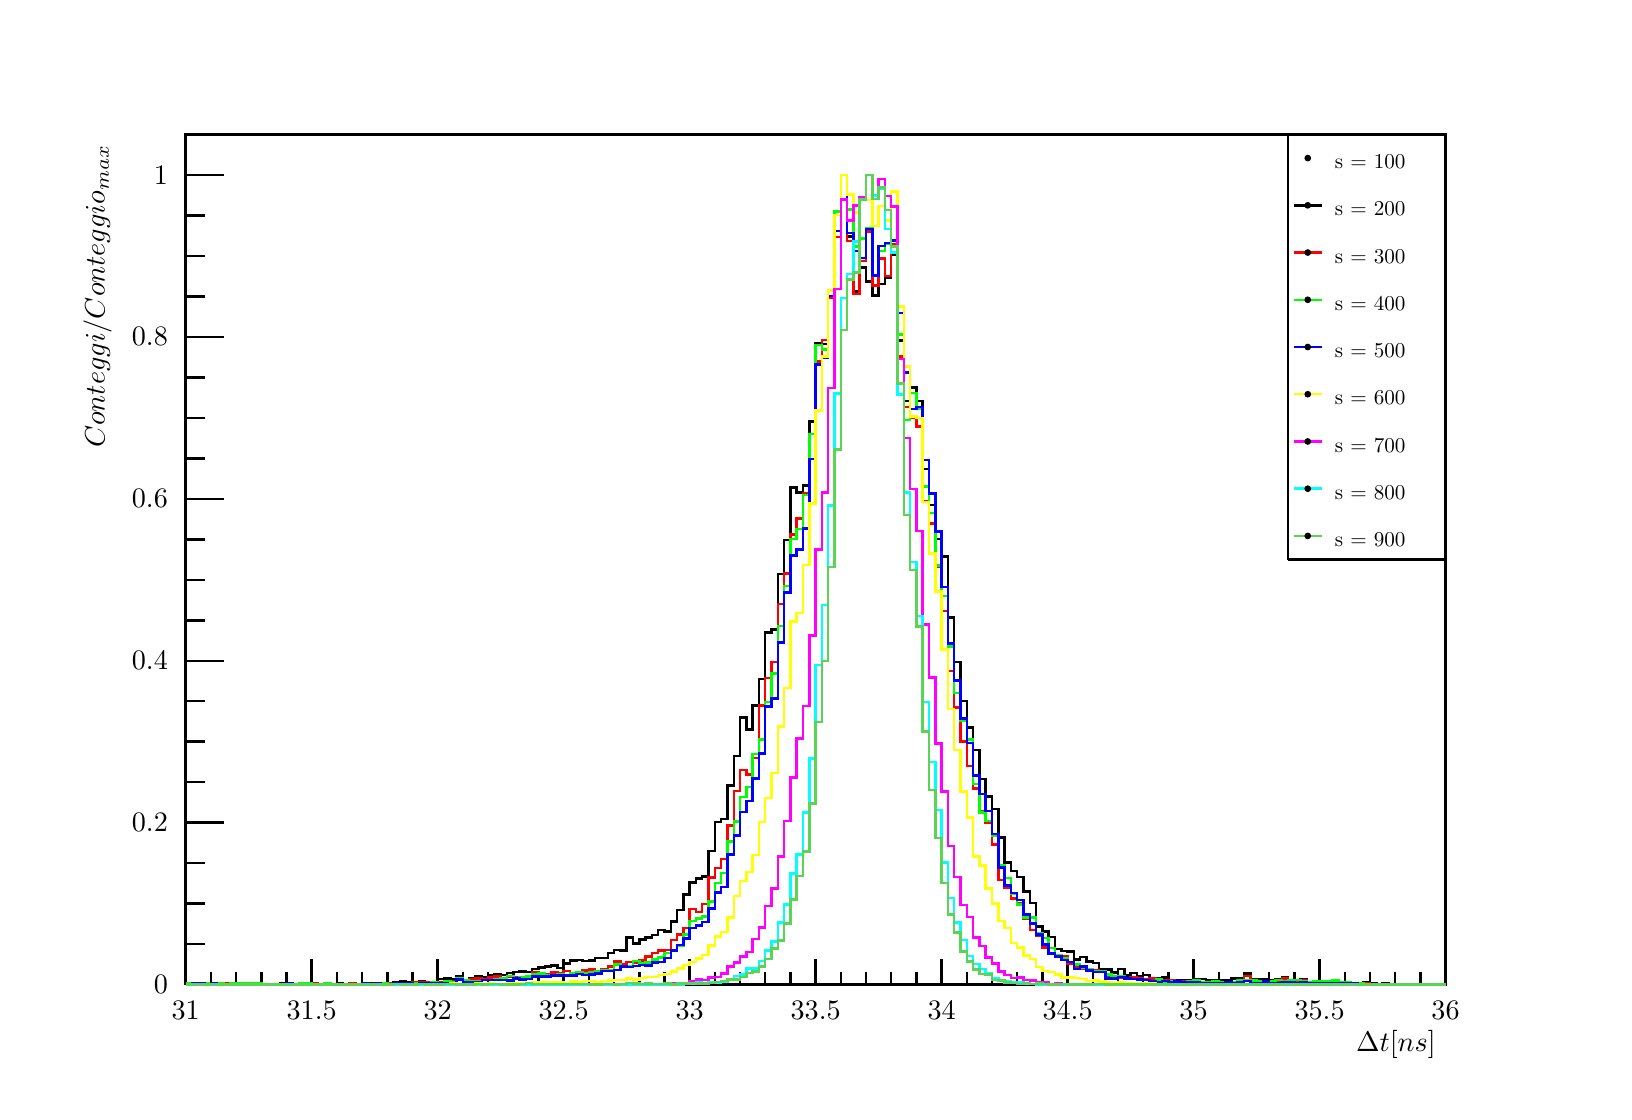
\begin{tikzpicture}
\pgfdeclareplotmark{cross} {
\pgfpathmoveto{\pgfpoint{-0.3\pgfplotmarksize}{\pgfplotmarksize}}
\pgfpathlineto{\pgfpoint{+0.3\pgfplotmarksize}{\pgfplotmarksize}}
\pgfpathlineto{\pgfpoint{+0.3\pgfplotmarksize}{0.3\pgfplotmarksize}}
\pgfpathlineto{\pgfpoint{+1\pgfplotmarksize}{0.3\pgfplotmarksize}}
\pgfpathlineto{\pgfpoint{+1\pgfplotmarksize}{-0.3\pgfplotmarksize}}
\pgfpathlineto{\pgfpoint{+0.3\pgfplotmarksize}{-0.3\pgfplotmarksize}}
\pgfpathlineto{\pgfpoint{+0.3\pgfplotmarksize}{-1.\pgfplotmarksize}}
\pgfpathlineto{\pgfpoint{-0.3\pgfplotmarksize}{-1.\pgfplotmarksize}}
\pgfpathlineto{\pgfpoint{-0.3\pgfplotmarksize}{-0.3\pgfplotmarksize}}
\pgfpathlineto{\pgfpoint{-1.\pgfplotmarksize}{-0.3\pgfplotmarksize}}
\pgfpathlineto{\pgfpoint{-1.\pgfplotmarksize}{0.3\pgfplotmarksize}}
\pgfpathlineto{\pgfpoint{-0.3\pgfplotmarksize}{0.3\pgfplotmarksize}}
\pgfpathclose
\pgfusepathqstroke
}
\pgfdeclareplotmark{cross*} {
\pgfpathmoveto{\pgfpoint{-0.3\pgfplotmarksize}{\pgfplotmarksize}}
\pgfpathlineto{\pgfpoint{+0.3\pgfplotmarksize}{\pgfplotmarksize}}
\pgfpathlineto{\pgfpoint{+0.3\pgfplotmarksize}{0.3\pgfplotmarksize}}
\pgfpathlineto{\pgfpoint{+1\pgfplotmarksize}{0.3\pgfplotmarksize}}
\pgfpathlineto{\pgfpoint{+1\pgfplotmarksize}{-0.3\pgfplotmarksize}}
\pgfpathlineto{\pgfpoint{+0.3\pgfplotmarksize}{-0.3\pgfplotmarksize}}
\pgfpathlineto{\pgfpoint{+0.3\pgfplotmarksize}{-1.\pgfplotmarksize}}
\pgfpathlineto{\pgfpoint{-0.3\pgfplotmarksize}{-1.\pgfplotmarksize}}
\pgfpathlineto{\pgfpoint{-0.3\pgfplotmarksize}{-0.3\pgfplotmarksize}}
\pgfpathlineto{\pgfpoint{-1.\pgfplotmarksize}{-0.3\pgfplotmarksize}}
\pgfpathlineto{\pgfpoint{-1.\pgfplotmarksize}{0.3\pgfplotmarksize}}
\pgfpathlineto{\pgfpoint{-0.3\pgfplotmarksize}{0.3\pgfplotmarksize}}
\pgfpathclose
\pgfusepathqfillstroke
}
\pgfdeclareplotmark{newstar} {
\pgfpathmoveto{\pgfqpoint{0pt}{\pgfplotmarksize}}
\pgfpathlineto{\pgfqpointpolar{44}{0.5\pgfplotmarksize}}
\pgfpathlineto{\pgfqpointpolar{18}{\pgfplotmarksize}}
\pgfpathlineto{\pgfqpointpolar{-20}{0.5\pgfplotmarksize}}
\pgfpathlineto{\pgfqpointpolar{-54}{\pgfplotmarksize}}
\pgfpathlineto{\pgfqpointpolar{-90}{0.5\pgfplotmarksize}}
\pgfpathlineto{\pgfqpointpolar{234}{\pgfplotmarksize}}
\pgfpathlineto{\pgfqpointpolar{198}{0.5\pgfplotmarksize}}
\pgfpathlineto{\pgfqpointpolar{162}{\pgfplotmarksize}}
\pgfpathlineto{\pgfqpointpolar{134}{0.5\pgfplotmarksize}}
\pgfpathclose
\pgfusepathqstroke
}
\pgfdeclareplotmark{newstar*} {
\pgfpathmoveto{\pgfqpoint{0pt}{\pgfplotmarksize}}
\pgfpathlineto{\pgfqpointpolar{44}{0.5\pgfplotmarksize}}
\pgfpathlineto{\pgfqpointpolar{18}{\pgfplotmarksize}}
\pgfpathlineto{\pgfqpointpolar{-20}{0.5\pgfplotmarksize}}
\pgfpathlineto{\pgfqpointpolar{-54}{\pgfplotmarksize}}
\pgfpathlineto{\pgfqpointpolar{-90}{0.5\pgfplotmarksize}}
\pgfpathlineto{\pgfqpointpolar{234}{\pgfplotmarksize}}
\pgfpathlineto{\pgfqpointpolar{198}{0.5\pgfplotmarksize}}
\pgfpathlineto{\pgfqpointpolar{162}{\pgfplotmarksize}}
\pgfpathlineto{\pgfqpointpolar{134}{0.5\pgfplotmarksize}}
\pgfpathclose
\pgfusepathqfillstroke
}
\definecolor{c}{rgb}{1,1,1};
\draw [color=c, fill=c] (0,0) rectangle (20,13.4957);
\draw [color=c, fill=c] (2,1.34957) rectangle (18,12.1461);
\definecolor{c}{rgb}{0,0,0};
\draw [c,line width=0.9] (2,1.34957) -- (2,12.1461) -- (18,12.1461) -- (18,1.34957) -- (2,1.34957);
\definecolor{c}{rgb}{1,1,1};
\draw [color=c, fill=c] (2,1.34957) rectangle (18,12.1461);
\definecolor{c}{rgb}{0,0,0};
\draw [c,line width=0.9] (2,1.34957) -- (2,12.1461) -- (18,12.1461) -- (18,1.34957) -- (2,1.34957);
\definecolor{c}{rgb}{1,1,1};
\draw [c,line width=0.9] (2,1.39147) -- (2.08,1.39147) -- (2.08,1.37471) -- (2.16,1.37471) -- (2.16,1.35795) -- (2.24,1.35795) -- (2.24,1.36633) -- (2.32,1.36633) -- (2.32,1.39985) -- (2.4,1.39985) -- (2.4,1.37471) -- (2.48,1.37471) -- (2.48,1.41661)
 -- (2.56,1.41661) -- (2.56,1.40823) -- (2.64,1.40823) -- (2.64,1.36633) -- (2.72,1.36633) -- (2.72,1.37471) -- (2.8,1.37471) -- (2.8,1.39147) -- (2.88,1.39147) -- (2.88,1.40823) -- (2.96,1.40823) -- (2.96,1.40823) -- (3.04,1.40823) -- (3.04,1.44175)
 -- (3.12,1.44175) -- (3.12,1.36633) -- (3.2,1.36633) -- (3.2,1.37471) -- (3.28,1.37471) -- (3.28,1.39147) -- (3.36,1.39147) -- (3.36,1.37471) -- (3.44,1.37471) -- (3.44,1.36633) -- (3.52,1.36633) -- (3.52,1.43337) -- (3.6,1.43337) -- (3.6,1.37471)
 -- (3.68,1.37471) -- (3.68,1.39985) -- (3.76,1.39985) -- (3.76,1.39985) -- (3.84,1.39985) -- (3.84,1.40823) -- (3.92,1.40823) -- (3.92,1.39985) -- (4,1.39985) -- (4,1.43337) -- (4.08,1.43337) -- (4.08,1.46689) -- (4.16,1.46689) -- (4.16,1.41661) --
 (4.24,1.41661) -- (4.24,1.36633) -- (4.32,1.36633) -- (4.32,1.42499) -- (4.4,1.42499) -- (4.4,1.44175) -- (4.48,1.44175) -- (4.48,1.47527) -- (4.56,1.47527) -- (4.56,1.45851) -- (4.64,1.45851) -- (4.64,1.48365) -- (4.72,1.48365) -- (4.72,1.41661) --
 (4.8,1.41661) -- (4.8,1.51717) -- (4.88,1.51717) -- (4.88,1.46689) -- (4.96,1.46689) -- (4.96,1.59259) -- (5.04,1.59259) -- (5.04,1.44175) -- (5.12,1.44175) -- (5.12,1.55907) -- (5.2,1.55907) -- (5.2,1.59259) -- (5.28,1.59259) -- (5.28,1.58421) --
 (5.36,1.58421) -- (5.36,1.50879) -- (5.44,1.50879) -- (5.44,1.7602) -- (5.52,1.7602) -- (5.52,1.65126) -- (5.6,1.65126) -- (5.6,1.55907) -- (5.68,1.55907) -- (5.68,1.56745) -- (5.76,1.56745) -- (5.76,1.74344) -- (5.84,1.74344) -- (5.84,1.75182) --
 (5.92,1.75182) -- (5.92,1.76858) -- (6,1.76858) -- (6,1.77696) -- (6.08,1.77696) -- (6.08,1.83562) -- (6.16,1.83562) -- (6.16,1.79372) -- (6.24,1.79372) -- (6.24,1.86076) -- (6.32,1.86076) -- (6.32,1.97808) -- (6.4,1.97808) -- (6.4,2.07864) --
 (6.48,2.07864) -- (6.48,2.12892) -- (6.56,2.12892) -- (6.56,1.96132) -- (6.64,1.96132) -- (6.64,2.07864) -- (6.72,2.07864) -- (6.72,1.97808) -- (6.8,1.97808) -- (6.8,2.06188) -- (6.88,2.06188) -- (6.88,2.22949) -- (6.96,2.22949) -- (6.96,2.22949) --
 (7.04,2.22949) -- (7.04,2.26301) -- (7.12,2.26301) -- (7.12,2.29653) -- (7.2,2.29653) -- (7.2,2.51441) -- (7.28,2.51441) -- (7.28,2.45575) -- (7.36,2.45575) -- (7.36,2.58983) -- (7.44,2.58983) -- (7.44,2.80772) -- (7.52,2.80772) -- (7.52,2.63173) --
 (7.6,2.63173) -- (7.6,2.76582) -- (7.68,2.76582) -- (7.68,2.79934) -- (7.76,2.79934) -- (7.76,3.12616) -- (7.84,3.12616) -- (7.84,3.11778) -- (7.92,3.11778) -- (7.92,3.20996) -- (8,3.20996) -- (8,3.16806) -- (8.08,3.16806) -- (8.08,3.67925) --
 (8.16,3.67925) -- (8.16,3.71277) -- (8.24,3.71277) -- (8.24,3.73791) -- (8.32,3.73791) -- (8.32,4.1234) -- (8.4,4.1234) -- (8.4,4.71001) -- (8.48,4.71001) -- (8.48,4.62621) -- (8.56,4.62621) -- (8.56,4.60107) -- (8.64,4.60107) -- (8.64,4.83571) --
 (8.72,4.83571) -- (8.72,5.50612) -- (8.8,5.50612) -- (8.8,5.27986) -- (8.88,5.27986) -- (8.88,6.20167) -- (8.96,6.20167) -- (8.96,6.50336) -- (9.04,6.50336) -- (9.04,6.68772) -- (9.12,6.68772) -- (9.12,6.79667) -- (9.2,6.79667) -- (9.2,7.00617) --
 (9.28,7.00617) -- (9.28,7.61792) -- (9.36,7.61792) -- (9.36,7.29109) -- (9.44,7.29109) -- (9.44,7.52574) -- (9.52,7.52574) -- (9.52,8.46431) -- (9.6,8.46431) -- (9.6,8.79114) -- (9.68,8.79114) -- (9.68,9.10959) -- (9.76,9.10959) -- (9.76,9.45317) --
 (9.84,9.45317) -- (9.84,9.11797) -- (9.92,9.11797) -- (9.92,9.36937) -- (10,9.36937) -- (10,10.4588) -- (10.08,10.4588) -- (10.08,10.7102) -- (10.16,10.7102) -- (10.16,10.9616) -- (10.24,10.9616) -- (10.24,11.632) -- (10.32,11.632) --
 (10.32,11.6152) -- (10.4,11.6152) -- (10.4,11.4225) -- (10.48,11.4225) -- (10.48,10.5677) -- (10.56,10.5677) -- (10.56,11.0957) -- (10.64,11.0957) -- (10.64,11.0035) -- (10.72,11.0035) -- (10.72,9.9057) -- (10.8,9.9057) -- (10.8,10.9029) --
 (10.88,10.9029) -- (10.88,10.4588) -- (10.96,10.4588) -- (10.96,10.8946) -- (11.04,10.8946) -- (11.04,10.1152) -- (11.12,10.1152) -- (11.12,9.36937) -- (11.2,9.36937) -- (11.2,9.26043) -- (11.28,9.26043) -- (11.28,9.41127) -- (11.36,9.41127) --
 (11.36,8.88332) -- (11.44,8.88332) -- (11.44,8.85818) -- (11.52,8.85818) -- (11.52,8.20453) -- (11.6,8.20453) -- (11.6,8.11235) -- (11.68,8.11235) -- (11.68,7.03969) -- (11.76,7.03969) -- (11.76,6.738) -- (11.84,6.738) -- (11.84,6.26034) --
 (11.92,6.26034) -- (11.92,5.95865) -- (12,5.95865) -- (12,5.36366) -- (12.08,5.36366) -- (12.08,5.1374) -- (12.16,5.1374) -- (12.16,5.10388) -- (12.24,5.10388) -- (12.24,4.60945) -- (12.32,4.60945) -- (12.32,4.21558) -- (12.4,4.21558) --
 (12.4,3.73791) -- (12.48,3.73791) -- (12.48,3.63735) -- (12.56,3.63735) -- (12.56,3.77981) -- (12.64,3.77981) -- (12.64,3.61221) -- (12.72,3.61221) -- (12.72,3.07588) -- (12.8,3.07588) -- (12.8,2.92504) -- (12.88,2.92504) -- (12.88,3.01722) --
 (12.96,3.01722) -- (12.96,2.79934) -- (13.04,2.79934) -- (13.04,2.59821) -- (13.12,2.59821) -- (13.12,2.42223) -- (13.2,2.42223) -- (13.2,2.40547) -- (13.28,2.40547) -- (13.28,2.12054) -- (13.36,2.12054) -- (13.36,2.17082) -- (13.44,2.17082) --
 (13.44,2.25463) -- (13.52,2.25463) -- (13.52,2.1792) -- (13.6,2.1792) -- (13.6,1.94456) -- (13.68,1.94456) -- (13.68,1.79372) -- (13.76,1.79372) -- (13.76,1.87752) -- (13.84,1.87752) -- (13.84,1.81886) -- (13.92,1.81886) -- (13.92,1.7183) --
 (14,1.7183) -- (14,1.66802) -- (14.08,1.66802) -- (14.08,1.85238) -- (14.16,1.85238) -- (14.16,1.6764) -- (14.24,1.6764) -- (14.24,1.66802) -- (14.32,1.66802) -- (14.32,1.70154) -- (14.4,1.70154) -- (14.4,1.65126) -- (14.48,1.65126) --
 (14.48,1.65126) -- (14.56,1.65126) -- (14.56,1.59259) -- (14.64,1.59259) -- (14.64,1.7602) -- (14.72,1.7602) -- (14.72,1.65964) -- (14.8,1.65964) -- (14.8,1.66802) -- (14.88,1.66802) -- (14.88,1.64288) -- (14.96,1.64288) -- (14.96,1.57583) --
 (15.04,1.57583) -- (15.04,1.59259) -- (15.12,1.59259) -- (15.12,1.69316) -- (15.2,1.69316) -- (15.2,1.60097) -- (15.28,1.60097) -- (15.28,1.69316) -- (15.36,1.69316) -- (15.36,1.60097) -- (15.44,1.60097) -- (15.44,1.87752) -- (15.52,1.87752) --
 (15.52,1.53393) -- (15.6,1.53393) -- (15.6,1.51717) -- (15.68,1.51717) -- (15.68,1.53393) -- (15.76,1.53393) -- (15.76,1.56745) -- (15.84,1.56745) -- (15.84,1.53393) -- (15.92,1.53393) -- (15.92,1.50879) -- (16,1.50879) -- (16,1.56745) --
 (16.08,1.56745) -- (16.08,1.53393) -- (16.16,1.53393) -- (16.16,1.45851) -- (16.24,1.45851) -- (16.24,1.56745) -- (16.32,1.56745) -- (16.32,1.45851) -- (16.4,1.45851) -- (16.4,1.47527) -- (16.48,1.47527) -- (16.48,1.45851) -- (16.56,1.45851) --
 (16.56,1.46689) -- (16.64,1.46689) -- (16.64,1.41661) -- (16.72,1.41661) -- (16.72,1.45013) -- (16.8,1.45013) -- (16.8,1.41661) -- (16.88,1.41661) -- (16.88,1.41661) -- (16.96,1.41661) -- (16.96,1.38309) -- (17.04,1.38309) -- (17.04,1.42499) --
 (17.12,1.42499) -- (17.12,1.37471) -- (17.2,1.37471) -- (17.2,1.37471) -- (17.28,1.37471) -- (17.28,1.39147) -- (17.36,1.39147) -- (17.36,1.37471) -- (17.44,1.37471) -- (17.44,1.37471) -- (17.52,1.37471) -- (17.52,1.39985) -- (17.6,1.39985) --
 (17.6,1.35795) -- (17.68,1.35795) -- (17.68,1.34957) -- (17.76,1.34957) -- (17.76,1.38309) -- (17.84,1.38309) -- (17.84,1.37471) -- (17.92,1.37471) -- (17.92,1.35795) -- (18,1.35795);
\definecolor{c}{rgb}{0,0,0};
\draw [c,line width=0.9] (2,1.34957) -- (18,1.34957);
\draw [anchor= east] (18,0.593811) node[scale=1.01821, color=c, rotate=0]{$\Delta t [ns]$};
\draw [c,line width=0.9] (2,1.67347) -- (2,1.34957);
\draw [c,line width=0.9] (2.32,1.51152) -- (2.32,1.34957);
\draw [c,line width=0.9] (2.64,1.51152) -- (2.64,1.34957);
\draw [c,line width=0.9] (2.96,1.51152) -- (2.96,1.34957);
\draw [c,line width=0.9] (3.28,1.51152) -- (3.28,1.34957);
\draw [c,line width=0.9] (3.6,1.67347) -- (3.6,1.34957);
\draw [c,line width=0.9] (3.92,1.51152) -- (3.92,1.34957);
\draw [c,line width=0.9] (4.24,1.51152) -- (4.24,1.34957);
\draw [c,line width=0.9] (4.56,1.51152) -- (4.56,1.34957);
\draw [c,line width=0.9] (4.88,1.51152) -- (4.88,1.34957);
\draw [c,line width=0.9] (5.2,1.67347) -- (5.2,1.34957);
\draw [c,line width=0.9] (5.52,1.51152) -- (5.52,1.34957);
\draw [c,line width=0.9] (5.84,1.51152) -- (5.84,1.34957);
\draw [c,line width=0.9] (6.16,1.51152) -- (6.16,1.34957);
\draw [c,line width=0.9] (6.48,1.51152) -- (6.48,1.34957);
\draw [c,line width=0.9] (6.8,1.67347) -- (6.8,1.34957);
\draw [c,line width=0.9] (7.12,1.51152) -- (7.12,1.34957);
\draw [c,line width=0.9] (7.44,1.51152) -- (7.44,1.34957);
\draw [c,line width=0.9] (7.76,1.51152) -- (7.76,1.34957);
\draw [c,line width=0.9] (8.08,1.51152) -- (8.08,1.34957);
\draw [c,line width=0.9] (8.4,1.67347) -- (8.4,1.34957);
\draw [c,line width=0.9] (8.72,1.51152) -- (8.72,1.34957);
\draw [c,line width=0.9] (9.04,1.51152) -- (9.04,1.34957);
\draw [c,line width=0.9] (9.36,1.51152) -- (9.36,1.34957);
\draw [c,line width=0.9] (9.68,1.51152) -- (9.68,1.34957);
\draw [c,line width=0.9] (10,1.67347) -- (10,1.34957);
\draw [c,line width=0.9] (10.32,1.51152) -- (10.32,1.34957);
\draw [c,line width=0.9] (10.64,1.51152) -- (10.64,1.34957);
\draw [c,line width=0.9] (10.96,1.51152) -- (10.96,1.34957);
\draw [c,line width=0.9] (11.28,1.51152) -- (11.28,1.34957);
\draw [c,line width=0.9] (11.6,1.67347) -- (11.6,1.34957);
\draw [c,line width=0.9] (11.92,1.51152) -- (11.92,1.34957);
\draw [c,line width=0.9] (12.24,1.51152) -- (12.24,1.34957);
\draw [c,line width=0.9] (12.56,1.51152) -- (12.56,1.34957);
\draw [c,line width=0.9] (12.88,1.51152) -- (12.88,1.34957);
\draw [c,line width=0.9] (13.2,1.67347) -- (13.2,1.34957);
\draw [c,line width=0.9] (13.52,1.51152) -- (13.52,1.34957);
\draw [c,line width=0.9] (13.84,1.51152) -- (13.84,1.34957);
\draw [c,line width=0.9] (14.16,1.51152) -- (14.16,1.34957);
\draw [c,line width=0.9] (14.48,1.51152) -- (14.48,1.34957);
\draw [c,line width=0.9] (14.8,1.67347) -- (14.8,1.34957);
\draw [c,line width=0.9] (15.12,1.51152) -- (15.12,1.34957);
\draw [c,line width=0.9] (15.44,1.51152) -- (15.44,1.34957);
\draw [c,line width=0.9] (15.76,1.51152) -- (15.76,1.34957);
\draw [c,line width=0.9] (16.08,1.51152) -- (16.08,1.34957);
\draw [c,line width=0.9] (16.4,1.67347) -- (16.4,1.34957);
\draw [c,line width=0.9] (16.72,1.51152) -- (16.72,1.34957);
\draw [c,line width=0.9] (17.04,1.51152) -- (17.04,1.34957);
\draw [c,line width=0.9] (17.36,1.51152) -- (17.36,1.34957);
\draw [c,line width=0.9] (17.68,1.51152) -- (17.68,1.34957);
\draw [c,line width=0.9] (18,1.67347) -- (18,1.34957);
\draw [anchor=base] (2,0.904212) node[scale=1.01821, color=c, rotate=0]{31};
\draw [anchor=base] (3.6,0.904212) node[scale=1.01821, color=c, rotate=0]{31.5};
\draw [anchor=base] (5.2,0.904212) node[scale=1.01821, color=c, rotate=0]{32};
\draw [anchor=base] (6.8,0.904212) node[scale=1.01821, color=c, rotate=0]{32.5};
\draw [anchor=base] (8.4,0.904212) node[scale=1.01821, color=c, rotate=0]{33};
\draw [anchor=base] (10,0.904212) node[scale=1.01821, color=c, rotate=0]{33.5};
\draw [anchor=base] (11.6,0.904212) node[scale=1.01821, color=c, rotate=0]{34};
\draw [anchor=base] (13.2,0.904212) node[scale=1.01821, color=c, rotate=0]{34.5};
\draw [anchor=base] (14.8,0.904212) node[scale=1.01821, color=c, rotate=0]{35};
\draw [anchor=base] (16.4,0.904212) node[scale=1.01821, color=c, rotate=0]{35.5};
\draw [anchor=base] (18,0.904212) node[scale=1.01821, color=c, rotate=0]{36};
\draw [c,line width=0.9] (2,1.34957) -- (2,12.1461);
\draw [anchor= east] (0.88,12.1461) node[scale=1.01821, color=c, rotate=90]{$Conteggi/Conteggio_{max}$};
\draw [c,line width=0.9] (2.48,1.34957) -- (2,1.34957);
\draw [c,line width=0.9] (2.24,1.86369) -- (2,1.86369);
\draw [c,line width=0.9] (2.24,2.37781) -- (2,2.37781);
\draw [c,line width=0.9] (2.24,2.89194) -- (2,2.89194);
\draw [c,line width=0.9] (2.48,3.40606) -- (2,3.40606);
\draw [c,line width=0.9] (2.24,3.92018) -- (2,3.92018);
\draw [c,line width=0.9] (2.24,4.4343) -- (2,4.4343);
\draw [c,line width=0.9] (2.24,4.94842) -- (2,4.94842);
\draw [c,line width=0.9] (2.48,5.46255) -- (2,5.46255);
\draw [c,line width=0.9] (2.24,5.97667) -- (2,5.97667);
\draw [c,line width=0.9] (2.24,6.49079) -- (2,6.49079);
\draw [c,line width=0.9] (2.24,7.00491) -- (2,7.00491);
\draw [c,line width=0.9] (2.48,7.51903) -- (2,7.51903);
\draw [c,line width=0.9] (2.24,8.03316) -- (2,8.03316);
\draw [c,line width=0.9] (2.24,8.54728) -- (2,8.54728);
\draw [c,line width=0.9] (2.24,9.0614) -- (2,9.0614);
\draw [c,line width=0.9] (2.48,9.57552) -- (2,9.57552);
\draw [c,line width=0.9] (2.24,10.0896) -- (2,10.0896);
\draw [c,line width=0.9] (2.24,10.6038) -- (2,10.6038);
\draw [c,line width=0.9] (2.24,11.1179) -- (2,11.1179);
\draw [c,line width=0.9] (2.48,11.632) -- (2,11.632);
\draw [c,line width=0.9] (2.48,11.632) -- (2,11.632);
\draw [anchor= east] (1.9,1.34957) node[scale=1.01821, color=c, rotate=0]{0};
\draw [anchor= east] (1.9,3.40606) node[scale=1.01821, color=c, rotate=0]{0.2};
\draw [anchor= east] (1.9,5.46255) node[scale=1.01821, color=c, rotate=0]{0.4};
\draw [anchor= east] (1.9,7.51903) node[scale=1.01821, color=c, rotate=0]{0.6};
\draw [anchor= east] (1.9,9.57552) node[scale=1.01821, color=c, rotate=0]{0.8};
\draw [anchor= east] (1.9,11.632) node[scale=1.01821, color=c, rotate=0]{1};
\draw [c,line width=0.9] (2,1.36049) -- (2.08,1.36049) -- (2.08,1.35776) -- (2.16,1.35776) -- (2.16,1.35776) -- (2.24,1.35776) -- (2.24,1.3523) -- (2.32,1.3523) -- (2.32,1.36869) -- (2.4,1.36869) -- (2.4,1.36049) -- (2.48,1.36049) -- (2.48,1.35776)
 -- (2.56,1.35776) -- (2.56,1.36049) -- (2.64,1.36049) -- (2.64,1.3523) -- (2.72,1.3523) -- (2.72,1.36596) -- (2.8,1.36596) -- (2.8,1.35776) -- (2.88,1.35776) -- (2.88,1.35776) -- (2.96,1.35776) -- (2.96,1.3523) -- (3.04,1.3523) -- (3.04,1.35503) --
 (3.12,1.35503) -- (3.12,1.35776) -- (3.2,1.35776) -- (3.2,1.36323) -- (3.28,1.36323) -- (3.28,1.35776) -- (3.36,1.35776) -- (3.36,1.35503) -- (3.44,1.35503) -- (3.44,1.36049) -- (3.52,1.36049) -- (3.52,1.35503) -- (3.6,1.35503) -- (3.6,1.35503) --
 (3.68,1.35503) -- (3.68,1.3523) -- (3.76,1.3523) -- (3.76,1.35503) -- (3.84,1.35503) -- (3.84,1.35776) -- (3.92,1.35776) -- (3.92,1.36596) -- (4,1.36596) -- (4,1.35503) -- (4.08,1.35503) -- (4.08,1.35776) -- (4.16,1.35776) -- (4.16,1.3523) --
 (4.24,1.3523) -- (4.24,1.36049) -- (4.32,1.36049) -- (4.32,1.36323) -- (4.4,1.36323) -- (4.4,1.36049) -- (4.48,1.36049) -- (4.48,1.36869) -- (4.56,1.36869) -- (4.56,1.36869) -- (4.64,1.36869) -- (4.64,1.37961) -- (4.72,1.37961) -- (4.72,1.38781) --
 (4.8,1.38781) -- (4.8,1.37415) -- (4.88,1.37415) -- (4.88,1.37688) -- (4.96,1.37688) -- (4.96,1.39054) -- (5.04,1.39054) -- (5.04,1.37961) -- (5.12,1.37961) -- (5.12,1.38507) -- (5.2,1.38507) -- (5.2,1.42058) -- (5.28,1.42058) -- (5.28,1.42604) --
 (5.36,1.42604) -- (5.36,1.42058) -- (5.44,1.42058) -- (5.44,1.45062) -- (5.52,1.45062) -- (5.52,1.40419) -- (5.6,1.40419) -- (5.6,1.4315) -- (5.68,1.4315) -- (5.68,1.45608) -- (5.76,1.45608) -- (5.76,1.44789) -- (5.84,1.44789) -- (5.84,1.47247) --
 (5.92,1.47247) -- (5.92,1.48339) -- (6,1.48339) -- (6,1.46974) -- (6.08,1.46974) -- (6.08,1.49432) -- (6.16,1.49432) -- (6.16,1.50797) -- (6.24,1.50797) -- (6.24,1.5189) -- (6.32,1.5189) -- (6.32,1.50797) -- (6.4,1.50797) -- (6.4,1.54621) --
 (6.48,1.54621) -- (6.48,1.56532) -- (6.56,1.56532) -- (6.56,1.57898) -- (6.64,1.57898) -- (6.64,1.59263) -- (6.72,1.59263) -- (6.72,1.56259) -- (6.8,1.56259) -- (6.8,1.61995) -- (6.88,1.61995) -- (6.88,1.65272) -- (6.96,1.65272) -- (6.96,1.66091) --
 (7.04,1.66091) -- (7.04,1.64726) -- (7.12,1.64726) -- (7.12,1.65818) -- (7.2,1.65818) -- (7.2,1.68822) -- (7.28,1.68822) -- (7.28,1.68822) -- (7.36,1.68822) -- (7.36,1.7483) -- (7.44,1.7483) -- (7.44,1.78927) -- (7.52,1.78927) -- (7.52,1.78108) --
 (7.6,1.78108) -- (7.6,1.94767) -- (7.68,1.94767) -- (7.68,1.87393) -- (7.76,1.87393) -- (7.76,1.92309) -- (7.84,1.92309) -- (7.84,1.94767) -- (7.92,1.94767) -- (7.92,1.98045) -- (8,1.98045) -- (8,2.04326) -- (8.08,2.04326) -- (8.08,2.02414) --
 (8.16,2.02414) -- (8.16,2.1525) -- (8.24,2.1525) -- (8.24,2.29725) -- (8.32,2.29725) -- (8.32,2.49662) -- (8.4,2.49662) -- (8.4,2.64682) -- (8.48,2.64682) -- (8.48,2.69871) -- (8.56,2.69871) -- (8.56,2.72329) -- (8.64,2.72329) -- (8.64,3.04829) --
 (8.72,3.04829) -- (8.72,3.41425) -- (8.8,3.41425) -- (8.8,3.44975) -- (8.88,3.44975) -- (8.88,3.88126) -- (8.96,3.88126) -- (8.96,4.25542) -- (9.04,4.25542) -- (9.04,4.74155) -- (9.12,4.74155) -- (9.12,4.58861) -- (9.2,4.58861) -- (9.2,4.89722) --
 (9.28,4.89722) -- (9.28,5.23314) -- (9.36,5.23314) -- (9.36,5.82031) -- (9.44,5.82031) -- (9.44,5.85855) -- (9.52,5.85855) -- (9.52,6.56589) -- (9.6,6.56589) -- (9.6,6.99467) -- (9.68,6.99467) -- (9.68,7.66105) -- (9.76,7.66105) -- (9.76,7.60097) --
 (9.84,7.60097) -- (9.84,7.68836) -- (9.92,7.68836) -- (9.92,8.49948) -- (10,8.49948) -- (10,9.49632) -- (10.08,9.49632) -- (10.08,9.48267) -- (10.16,9.48267) -- (10.16,10.1572) -- (10.24,10.1572) -- (10.24,11.1677) -- (10.32,11.1677) --
 (10.32,11.632) -- (10.4,11.632) -- (10.4,10.8509) -- (10.48,10.8509) -- (10.48,10.1545) -- (10.56,10.1545) -- (10.56,10.4549) -- (10.64,10.4549) -- (10.64,10.2774) -- (10.72,10.2774) -- (10.72,10.0999) -- (10.8,10.0999) -- (10.8,10.2474) --
 (10.88,10.2474) -- (10.88,10.3266) -- (10.96,10.3266) -- (10.96,10.6242) -- (11.04,10.6242) -- (11.04,9.53183) -- (11.12,9.53183) -- (11.12,8.75893) -- (11.2,8.75893) -- (11.2,8.93099) -- (11.28,8.93099) -- (11.28,8.75893) -- (11.36,8.75893) --
 (11.36,7.89592) -- (11.44,7.89592) -- (11.44,7.44256) -- (11.52,7.44256) -- (11.52,7.01106) -- (11.6,7.01106) -- (11.6,6.78711) -- (11.68,6.78711) -- (11.68,6.01422) -- (11.76,6.01422) -- (11.76,5.44889) -- (11.84,5.44889) -- (11.84,4.95457) --
 (11.92,4.95457) -- (11.92,4.61592) -- (12,4.61592) -- (12,4.32916) -- (12.08,4.32916) -- (12.08,3.96319) -- (12.16,3.96319) -- (12.16,3.73925) -- (12.24,3.73925) -- (12.24,3.57811) -- (12.32,3.57811) -- (12.32,3.21761) -- (12.4,3.21761) --
 (12.4,2.89808) -- (12.48,2.89808) -- (12.48,2.79157) -- (12.56,2.79157) -- (12.56,2.7151) -- (12.64,2.7151) -- (12.64,2.53485) -- (12.72,2.53485) -- (12.72,2.38737) -- (12.8,2.38737) -- (12.8,2.08696) -- (12.88,2.08696) -- (12.88,2.02687) --
 (12.96,2.02687) -- (12.96,1.95313) -- (13.04,1.95313) -- (13.04,1.8002) -- (13.12,1.8002) -- (13.12,1.77835) -- (13.2,1.77835) -- (13.2,1.77015) -- (13.28,1.77015) -- (13.28,1.6691) -- (13.36,1.6691) -- (13.36,1.70188) -- (13.44,1.70188) --
 (13.44,1.64179) -- (13.52,1.64179) -- (13.52,1.62541) -- (13.6,1.62541) -- (13.6,1.54074) -- (13.68,1.54074) -- (13.68,1.54348) -- (13.76,1.54348) -- (13.76,1.50524) -- (13.84,1.50524) -- (13.84,1.54621) -- (13.92,1.54621) -- (13.92,1.46427) --
 (14,1.46427) -- (14,1.49978) -- (14.08,1.49978) -- (14.08,1.46154) -- (14.16,1.46154) -- (14.16,1.47247) -- (14.24,1.47247) -- (14.24,1.42058) -- (14.32,1.42058) -- (14.32,1.42877) -- (14.4,1.42877) -- (14.4,1.4397) -- (14.48,1.4397) --
 (14.48,1.39054) -- (14.56,1.39054) -- (14.56,1.40692) -- (14.64,1.40692) -- (14.64,1.40965) -- (14.72,1.40965) -- (14.72,1.40965) -- (14.8,1.40965) -- (14.8,1.41785) -- (14.88,1.41785) -- (14.88,1.42331) -- (14.96,1.42331) -- (14.96,1.40692) --
 (15.04,1.40692) -- (15.04,1.40965) -- (15.12,1.40965) -- (15.12,1.39873) -- (15.2,1.39873) -- (15.2,1.40692) -- (15.28,1.40692) -- (15.28,1.42877) -- (15.36,1.42877) -- (15.36,1.42604) -- (15.44,1.42604) -- (15.44,1.49159) -- (15.52,1.49159) --
 (15.52,1.41238) -- (15.6,1.41238) -- (15.6,1.42058) -- (15.68,1.42058) -- (15.68,1.41512) -- (15.76,1.41512) -- (15.76,1.40692) -- (15.84,1.40692) -- (15.84,1.41785) -- (15.92,1.41785) -- (15.92,1.43696) -- (16,1.43696) -- (16,1.40146) --
 (16.08,1.40146) -- (16.08,1.39327) -- (16.16,1.39327) -- (16.16,1.41238) -- (16.24,1.41238) -- (16.24,1.38507) -- (16.32,1.38507) -- (16.32,1.38781) -- (16.4,1.38781) -- (16.4,1.39327) -- (16.48,1.39327) -- (16.48,1.39327) -- (16.56,1.39327) --
 (16.56,1.37961) -- (16.64,1.37961) -- (16.64,1.36323) -- (16.72,1.36323) -- (16.72,1.37961) -- (16.8,1.37961) -- (16.8,1.37142) -- (16.88,1.37142) -- (16.88,1.35776) -- (16.96,1.35776) -- (16.96,1.37415) -- (17.04,1.37415) -- (17.04,1.36596) --
 (17.12,1.36596) -- (17.12,1.35503) -- (17.2,1.35503) -- (17.2,1.36596) -- (17.28,1.36596) -- (17.28,1.35503) -- (17.36,1.35503) -- (17.36,1.35503) -- (17.44,1.35503) -- (17.44,1.35503) -- (17.52,1.35503) -- (17.52,1.3523) -- (17.6,1.3523) --
 (17.6,1.35776) -- (17.68,1.35776) -- (17.68,1.35503) -- (17.76,1.35503) -- (17.76,1.35503) -- (17.84,1.35503) -- (17.84,1.3523) -- (17.92,1.3523) -- (17.92,1.34957) -- (18,1.34957);
\definecolor{c}{rgb}{1,0,0};
\draw [c,line width=0.9] (2,1.36505) -- (2.08,1.36505) -- (2.08,1.35925) -- (2.16,1.35925) -- (2.16,1.35538) -- (2.24,1.35538) -- (2.24,1.36505) -- (2.32,1.36505) -- (2.32,1.34957) -- (2.4,1.34957) -- (2.4,1.35731) -- (2.48,1.35731) -- (2.48,1.36505)
 -- (2.56,1.36505) -- (2.56,1.35731) -- (2.64,1.35731) -- (2.64,1.35538) -- (2.72,1.35538) -- (2.72,1.35925) -- (2.8,1.35925) -- (2.8,1.35538) -- (2.88,1.35538) -- (2.88,1.35344) -- (2.96,1.35344) -- (2.96,1.35731) -- (3.04,1.35731) -- (3.04,1.35344)
 -- (3.12,1.35344) -- (3.12,1.35151) -- (3.2,1.35151) -- (3.2,1.35925) -- (3.28,1.35925) -- (3.28,1.35538) -- (3.36,1.35538) -- (3.36,1.35538) -- (3.44,1.35538) -- (3.44,1.36118) -- (3.52,1.36118) -- (3.52,1.35925) -- (3.6,1.35925) -- (3.6,1.36312)
 -- (3.68,1.36312) -- (3.68,1.35538) -- (3.76,1.35538) -- (3.76,1.35925) -- (3.84,1.35925) -- (3.84,1.35731) -- (3.92,1.35731) -- (3.92,1.35731) -- (4,1.35731) -- (4,1.35344) -- (4.08,1.35344) -- (4.08,1.36312) -- (4.16,1.36312) -- (4.16,1.35731) --
 (4.24,1.35731) -- (4.24,1.35344) -- (4.32,1.35344) -- (4.32,1.35731) -- (4.4,1.35731) -- (4.4,1.35925) -- (4.48,1.35925) -- (4.48,1.36118) -- (4.56,1.36118) -- (4.56,1.36118) -- (4.64,1.36118) -- (4.64,1.35925) -- (4.72,1.35925) -- (4.72,1.36698) --
 (4.8,1.36698) -- (4.8,1.35731) -- (4.88,1.35731) -- (4.88,1.37666) -- (4.96,1.37666) -- (4.96,1.37666) -- (5.04,1.37666) -- (5.04,1.38246) -- (5.12,1.38246) -- (5.12,1.36698) -- (5.2,1.36698) -- (5.2,1.37859) -- (5.28,1.37859) -- (5.28,1.37859) --
 (5.36,1.37859) -- (5.36,1.38633) -- (5.44,1.38633) -- (5.44,1.41149) -- (5.52,1.41149) -- (5.52,1.38053) -- (5.6,1.38053) -- (5.6,1.41729) -- (5.68,1.41729) -- (5.68,1.4289) -- (5.76,1.4289) -- (5.76,1.41536) -- (5.84,1.41536) -- (5.84,1.43858) --
 (5.92,1.43858) -- (5.92,1.45019) -- (6,1.45019) -- (6,1.4231) -- (6.08,1.4231) -- (6.08,1.44632) -- (6.16,1.44632) -- (6.16,1.43858) -- (6.24,1.43858) -- (6.24,1.41923) -- (6.32,1.41923) -- (6.32,1.45212) -- (6.4,1.45212) -- (6.4,1.5005) --
 (6.48,1.5005) -- (6.48,1.45986) -- (6.56,1.45986) -- (6.56,1.48502) -- (6.64,1.48502) -- (6.64,1.50243) -- (6.72,1.50243) -- (6.72,1.49469) -- (6.8,1.49469) -- (6.8,1.52178) -- (6.88,1.52178) -- (6.88,1.47921) -- (6.96,1.47921) -- (6.96,1.5063) --
 (7.04,1.5063) -- (7.04,1.52952) -- (7.12,1.52952) -- (7.12,1.5392) -- (7.2,1.5392) -- (7.2,1.51211) -- (7.28,1.51211) -- (7.28,1.54694) -- (7.36,1.54694) -- (7.36,1.58177) -- (7.44,1.58177) -- (7.44,1.64175) -- (7.52,1.64175) -- (7.52,1.60499) --
 (7.6,1.60499) -- (7.6,1.63982) -- (7.68,1.63982) -- (7.68,1.6224) -- (7.76,1.6224) -- (7.76,1.65723) -- (7.84,1.65723) -- (7.84,1.70561) -- (7.92,1.70561) -- (7.92,1.75204) -- (8,1.75204) -- (8,1.78107) -- (8.08,1.78107) -- (8.08,1.78881) --
 (8.16,1.78881) -- (8.16,1.91652) -- (8.24,1.91652) -- (8.24,1.98424) -- (8.32,1.98424) -- (8.32,2.06551) -- (8.4,2.06551) -- (8.4,2.30738) -- (8.48,2.30738) -- (8.48,2.27062) -- (8.56,2.27062) -- (8.56,2.37124) -- (8.64,2.37124) -- (8.64,2.70986) --
 (8.72,2.70986) -- (8.72,2.82982) -- (8.8,2.82982) -- (8.8,2.94399) -- (8.88,2.94399) -- (8.88,3.36775) -- (8.96,3.36775) -- (8.96,3.81085) -- (9.04,3.81085) -- (9.04,4.07595) -- (9.12,4.07595) -- (9.12,4.01596) -- (9.2,4.01596) -- (9.2,4.22881) --
 (9.28,4.22881) -- (9.28,4.89637) -- (9.36,4.89637) -- (9.36,5.2466) -- (9.44,5.2466) -- (9.44,5.44784) -- (9.52,5.44784) -- (9.52,6.18506) -- (9.6,6.18506) -- (9.6,6.57206) -- (9.68,6.57206) -- (9.68,7.06354) -- (9.76,7.06354) -- (9.76,7.26671) --
 (9.84,7.26671) -- (9.84,7.59566) -- (9.92,7.59566) -- (9.92,8.34449) -- (10,8.34449) -- (10,9.26167) -- (10.08,9.26167) -- (10.08,9.53644) -- (10.16,9.53644) -- (10.16,10.0763) -- (10.24,10.0763) -- (10.24,10.8445) -- (10.32,10.8445) --
 (10.32,11.632) -- (10.4,11.632) -- (10.4,10.7961) -- (10.48,10.7961) -- (10.48,10.1227) -- (10.56,10.1227) -- (10.56,10.5368) -- (10.64,10.5368) -- (10.64,10.9141) -- (10.72,10.9141) -- (10.72,10.2292) -- (10.8,10.2292) -- (10.8,10.5697) --
 (10.88,10.5697) -- (10.88,10.3511) -- (10.96,10.3511) -- (10.96,10.7497) -- (11.04,10.7497) -- (11.04,9.32746) -- (11.12,9.32746) -- (11.12,8.68505) -- (11.2,8.68505) -- (11.2,8.54766) -- (11.28,8.54766) -- (11.28,8.43931) -- (11.36,8.43931) --
 (11.36,7.48343) -- (11.44,7.48343) -- (11.44,7.20673) -- (11.52,7.20673) -- (11.52,6.65333) -- (11.6,6.65333) -- (11.6,6.09412) -- (11.68,6.09412) -- (11.68,5.33368) -- (11.76,5.33368) -- (11.76,4.87122) -- (11.84,4.87122) -- (11.84,4.43972) --
 (11.92,4.43972) -- (11.92,4.12819) -- (12,4.12819) -- (12,3.84181) -- (12.08,3.84181) -- (12.08,3.55157) -- (12.16,3.55157) -- (12.16,3.40064) -- (12.24,3.40064) -- (12.24,3.13168) -- (12.32,3.13168) -- (12.32,2.6789) -- (12.4,2.6789) --
 (12.4,2.58602) -- (12.48,2.58602) -- (12.48,2.44476) -- (12.56,2.44476) -- (12.56,2.37898) -- (12.64,2.37898) -- (12.64,2.18741) -- (12.72,2.18741) -- (12.72,2.04229) -- (12.8,2.04229) -- (12.8,1.96489) -- (12.88,1.96489) -- (12.88,1.81977) --
 (12.96,1.81977) -- (12.96,1.7385) -- (13.04,1.7385) -- (13.04,1.71528) -- (13.12,1.71528) -- (13.12,1.71334) -- (13.2,1.71334) -- (13.2,1.6166) -- (13.28,1.6166) -- (13.28,1.58177) -- (13.36,1.58177) -- (13.36,1.545) -- (13.44,1.545) --
 (13.44,1.53533) -- (13.52,1.53533) -- (13.52,1.52952) -- (13.6,1.52952) -- (13.6,1.51017) -- (13.68,1.51017) -- (13.68,1.4676) -- (13.76,1.4676) -- (13.76,1.43664) -- (13.84,1.43664) -- (13.84,1.43277) -- (13.92,1.43277) -- (13.92,1.43471) --
 (14,1.43471) -- (14,1.44245) -- (14.08,1.44245) -- (14.08,1.42503) -- (14.16,1.42503) -- (14.16,1.41342) -- (14.24,1.41342) -- (14.24,1.42697) -- (14.32,1.42697) -- (14.32,1.39988) -- (14.4,1.39988) -- (14.4,1.40762) -- (14.48,1.40762) --
 (14.48,1.40762) -- (14.56,1.40762) -- (14.56,1.37859) -- (14.64,1.37859) -- (14.64,1.39407) -- (14.72,1.39407) -- (14.72,1.36698) -- (14.8,1.36698) -- (14.8,1.38633) -- (14.88,1.38633) -- (14.88,1.38053) -- (14.96,1.38053) -- (14.96,1.37472) --
 (15.04,1.37472) -- (15.04,1.39601) -- (15.12,1.39601) -- (15.12,1.38246) -- (15.2,1.38246) -- (15.2,1.38246) -- (15.28,1.38246) -- (15.28,1.37279) -- (15.36,1.37279) -- (15.36,1.38827) -- (15.44,1.38827) -- (15.44,1.45793) -- (15.52,1.45793) --
 (15.52,1.40181) -- (15.6,1.40181) -- (15.6,1.39794) -- (15.68,1.39794) -- (15.68,1.37859) -- (15.76,1.37859) -- (15.76,1.38246) -- (15.84,1.38246) -- (15.84,1.39794) -- (15.92,1.39794) -- (15.92,1.42503) -- (16,1.42503) -- (16,1.39988) --
 (16.08,1.39988) -- (16.08,1.38633) -- (16.16,1.38633) -- (16.16,1.40955) -- (16.24,1.40955) -- (16.24,1.38053) -- (16.32,1.38053) -- (16.32,1.39794) -- (16.4,1.39794) -- (16.4,1.35925) -- (16.48,1.35925) -- (16.48,1.37085) -- (16.56,1.37085) --
 (16.56,1.38053) -- (16.64,1.38053) -- (16.64,1.37279) -- (16.72,1.37279) -- (16.72,1.37279) -- (16.8,1.37279) -- (16.8,1.36118) -- (16.88,1.36118) -- (16.88,1.36312) -- (16.96,1.36312) -- (16.96,1.36118) -- (17.04,1.36118) -- (17.04,1.35925) --
 (17.12,1.35925) -- (17.12,1.35731) -- (17.2,1.35731) -- (17.2,1.35344) -- (17.28,1.35344) -- (17.28,1.34957) -- (17.36,1.34957) -- (17.36,1.35731) -- (17.44,1.35731) -- (17.44,1.35151) -- (17.52,1.35151) -- (17.52,1.34957) -- (17.6,1.34957) --
 (17.6,1.34957) -- (17.68,1.34957) -- (17.68,1.35151) -- (17.76,1.35151) -- (17.76,1.35151) -- (17.84,1.35151) -- (17.84,1.34957) -- (17.92,1.34957) -- (17.92,1.35151) -- (18,1.35151);
\definecolor{c}{rgb}{0,1,0};
\draw [c,line width=0.9] (2,1.36071) -- (2.08,1.36071) -- (2.08,1.36071) -- (2.16,1.36071) -- (2.16,1.3623) -- (2.24,1.3623) -- (2.24,1.36707) -- (2.32,1.36707) -- (2.32,1.36071) -- (2.4,1.36071) -- (2.4,1.3623) -- (2.48,1.3623) -- (2.48,1.35912) --
 (2.56,1.35912) -- (2.56,1.36071) -- (2.64,1.36071) -- (2.64,1.36071) -- (2.72,1.36071) -- (2.72,1.3623) -- (2.8,1.3623) -- (2.8,1.36389) -- (2.88,1.36389) -- (2.88,1.3623) -- (2.96,1.3623) -- (2.96,1.35594) -- (3.04,1.35594) -- (3.04,1.35594) --
 (3.12,1.35594) -- (3.12,1.35753) -- (3.2,1.35753) -- (3.2,1.35753) -- (3.28,1.35753) -- (3.28,1.35434) -- (3.36,1.35434) -- (3.36,1.35753) -- (3.44,1.35753) -- (3.44,1.36389) -- (3.52,1.36389) -- (3.52,1.36548) -- (3.6,1.36548) -- (3.6,1.35116) --
 (3.68,1.35116) -- (3.68,1.35434) -- (3.76,1.35434) -- (3.76,1.3623) -- (3.84,1.3623) -- (3.84,1.35275) -- (3.92,1.35275) -- (3.92,1.35753) -- (4,1.35753) -- (4,1.35594) -- (4.08,1.35594) -- (4.08,1.35434) -- (4.16,1.35434) -- (4.16,1.35753) --
 (4.24,1.35753) -- (4.24,1.3623) -- (4.32,1.3623) -- (4.32,1.35912) -- (4.4,1.35912) -- (4.4,1.35275) -- (4.48,1.35275) -- (4.48,1.36071) -- (4.56,1.36071) -- (4.56,1.35912) -- (4.64,1.35912) -- (4.64,1.37185) -- (4.72,1.37185) -- (4.72,1.3623) --
 (4.8,1.3623) -- (4.8,1.36389) -- (4.88,1.36389) -- (4.88,1.36707) -- (4.96,1.36707) -- (4.96,1.37026) -- (5.04,1.37026) -- (5.04,1.36866) -- (5.12,1.36866) -- (5.12,1.37821) -- (5.2,1.37821) -- (5.2,1.37185) -- (5.28,1.37185) -- (5.28,1.39094) --
 (5.36,1.39094) -- (5.36,1.37503) -- (5.44,1.37503) -- (5.44,1.4339) -- (5.52,1.4339) -- (5.52,1.3989) -- (5.6,1.3989) -- (5.6,1.39253) -- (5.68,1.39253) -- (5.68,1.39572) -- (5.76,1.39572) -- (5.76,1.40845) -- (5.84,1.40845) -- (5.84,1.40845) --
 (5.92,1.40845) -- (5.92,1.4164) -- (6,1.4164) -- (6,1.42595) -- (6.08,1.42595) -- (6.08,1.45618) -- (6.16,1.45618) -- (6.16,1.42754) -- (6.24,1.42754) -- (6.24,1.44027) -- (6.32,1.44027) -- (6.32,1.453) -- (6.4,1.453) -- (6.4,1.48164) --
 (6.48,1.48164) -- (6.48,1.49119) -- (6.56,1.49119) -- (6.56,1.47209) -- (6.64,1.47209) -- (6.64,1.4705) -- (6.72,1.4705) -- (6.72,1.47528) -- (6.8,1.47528) -- (6.8,1.45618) -- (6.88,1.45618) -- (6.88,1.49278) -- (6.96,1.49278) -- (6.96,1.51028) --
 (7.04,1.51028) -- (7.04,1.48801) -- (7.12,1.48801) -- (7.12,1.51187) -- (7.2,1.51187) -- (7.2,1.52142) -- (7.28,1.52142) -- (7.28,1.53097) -- (7.36,1.53097) -- (7.36,1.53733) -- (7.44,1.53733) -- (7.44,1.60576) -- (7.52,1.60576) -- (7.52,1.58666) --
 (7.6,1.58666) -- (7.6,1.58825) -- (7.68,1.58825) -- (7.68,1.64872) -- (7.76,1.64872) -- (7.76,1.62485) -- (7.84,1.62485) -- (7.84,1.63122) -- (7.92,1.63122) -- (7.92,1.66622) -- (8,1.66622) -- (8,1.69327) -- (8.08,1.69327) -- (8.08,1.75056) --
 (8.16,1.75056) -- (8.16,1.77602) -- (8.24,1.77602) -- (8.24,1.84921) -- (8.32,1.84921) -- (8.32,1.98606) -- (8.4,1.98606) -- (8.4,2.1595) -- (8.48,2.1595) -- (8.48,2.19132) -- (8.56,2.19132) -- (8.56,2.21201) -- (8.64,2.21201) -- (8.64,2.40773) --
 (8.72,2.40773) -- (8.72,2.64005) -- (8.8,2.64005) -- (8.8,2.76416) -- (8.88,2.76416) -- (8.88,3.16515) -- (8.96,3.16515) -- (8.96,3.42292) -- (9.04,3.42292) -- (9.04,3.73162) -- (9.12,3.73162) -- (9.12,3.85892) -- (9.2,3.85892) -- (9.2,4.27741) --
 (9.28,4.27741) -- (9.28,4.46517) -- (9.36,4.46517) -- (9.36,4.94095) -- (9.44,4.94095) -- (9.44,5.29897) -- (9.52,5.29897) -- (9.52,5.90681) -- (9.6,5.90681) -- (9.6,6.41441) -- (9.68,6.41441) -- (9.68,7.00953) -- (9.76,7.00953) -- (9.76,7.13364) --
 (9.84,7.13364) -- (9.84,7.56963) -- (9.92,7.56963) -- (9.92,8.33978) -- (10,8.33978) -- (10,9.47273) -- (10.08,9.47273) -- (10.08,9.41385) -- (10.16,9.41385) -- (10.16,10.1649) -- (10.24,10.1649) -- (10.24,11.1706) -- (10.32,11.1706) --
 (10.32,11.632) -- (10.4,11.632) -- (10.4,11.1912) -- (10.48,11.1912) -- (10.48,10.7218) -- (10.56,10.7218) -- (10.56,10.8269) -- (10.64,10.8269) -- (10.64,10.9526) -- (10.72,10.9526) -- (10.72,10.3606) -- (10.8,10.3606) -- (10.8,10.6661) --
 (10.88,10.6661) -- (10.88,10.7552) -- (10.96,10.7552) -- (10.96,10.7282) -- (11.04,10.7282) -- (11.04,9.60321) -- (11.12,9.60321) -- (11.12,8.52277) -- (11.2,8.52277) -- (11.2,8.8617) -- (11.28,8.8617) -- (11.28,8.66598) -- (11.36,8.66598) --
 (11.36,7.67465) -- (11.44,7.67465) -- (11.44,7.33732) -- (11.52,7.33732) -- (11.52,6.67219) -- (11.6,6.67219) -- (11.6,6.28234) -- (11.68,6.28234) -- (11.68,5.64426) -- (11.76,5.64426) -- (11.76,5.05392) -- (11.84,5.05392) -- (11.84,4.70385) --
 (11.92,4.70385) -- (11.92,4.4604) -- (12,4.4604) -- (12,3.89711) -- (12.08,3.89711) -- (12.08,3.53749) -- (12.16,3.53749) -- (12.16,3.42929) -- (12.24,3.42929) -- (12.24,3.23675) -- (12.32,3.23675) -- (12.32,2.86441) -- (12.4,2.86441) --
 (12.4,2.70051) -- (12.48,2.70051) -- (12.48,2.50161) -- (12.56,2.50161) -- (12.56,2.36477) -- (12.64,2.36477) -- (12.64,2.19928) -- (12.72,2.19928) -- (12.72,2.20087) -- (12.8,2.20087) -- (12.8,2.00038) -- (12.88,2.00038) -- (12.88,1.94309) --
 (12.96,1.94309) -- (12.96,1.8158) -- (13.04,1.8158) -- (13.04,1.71873) -- (13.12,1.71873) -- (13.12,1.68532) -- (13.2,1.68532) -- (13.2,1.63758) -- (13.28,1.63758) -- (13.28,1.60416) -- (13.36,1.60416) -- (13.36,1.55961) -- (13.44,1.55961) --
 (13.44,1.54529) -- (13.52,1.54529) -- (13.52,1.52301) -- (13.6,1.52301) -- (13.6,1.52142) -- (13.68,1.52142) -- (13.68,1.47687) -- (13.76,1.47687) -- (13.76,1.46096) -- (13.84,1.46096) -- (13.84,1.45618) -- (13.92,1.45618) -- (13.92,1.43072) --
 (14,1.43072) -- (14,1.42277) -- (14.08,1.42277) -- (14.08,1.42118) -- (14.16,1.42118) -- (14.16,1.40845) -- (14.24,1.40845) -- (14.24,1.39731) -- (14.32,1.39731) -- (14.32,1.41163) -- (14.4,1.41163) -- (14.4,1.38617) -- (14.48,1.38617) --
 (14.48,1.39253) -- (14.56,1.39253) -- (14.56,1.39253) -- (14.64,1.39253) -- (14.64,1.3798) -- (14.72,1.3798) -- (14.72,1.39412) -- (14.8,1.39412) -- (14.8,1.40049) -- (14.88,1.40049) -- (14.88,1.38299) -- (14.96,1.38299) -- (14.96,1.38299) --
 (15.04,1.38299) -- (15.04,1.38776) -- (15.12,1.38776) -- (15.12,1.37344) -- (15.2,1.37344) -- (15.2,1.38458) -- (15.28,1.38458) -- (15.28,1.3798) -- (15.36,1.3798) -- (15.36,1.3989) -- (15.44,1.3989) -- (15.44,1.41004) -- (15.52,1.41004) --
 (15.52,1.40049) -- (15.6,1.40049) -- (15.6,1.38617) -- (15.68,1.38617) -- (15.68,1.39412) -- (15.76,1.39412) -- (15.76,1.39412) -- (15.84,1.39412) -- (15.84,1.40526) -- (15.92,1.40526) -- (15.92,1.38776) -- (16,1.38776) -- (16,1.40685) --
 (16.08,1.40685) -- (16.08,1.40685) -- (16.16,1.40685) -- (16.16,1.39412) -- (16.24,1.39412) -- (16.24,1.38299) -- (16.32,1.38299) -- (16.32,1.39731) -- (16.4,1.39731) -- (16.4,1.38617) -- (16.48,1.38617) -- (16.48,1.39412) -- (16.56,1.39412) --
 (16.56,1.40049) -- (16.64,1.40049) -- (16.64,1.3798) -- (16.72,1.3798) -- (16.72,1.38139) -- (16.8,1.38139) -- (16.8,1.37026) -- (16.88,1.37026) -- (16.88,1.36548) -- (16.96,1.36548) -- (16.96,1.35434) -- (17.04,1.35434) -- (17.04,1.35912) --
 (17.12,1.35912) -- (17.12,1.35594) -- (17.2,1.35594) -- (17.2,1.35594) -- (17.28,1.35594) -- (17.28,1.35594) -- (17.36,1.35594) -- (17.36,1.35753) -- (17.44,1.35753) -- (17.44,1.35594) -- (17.52,1.35594) -- (17.52,1.35275) -- (17.6,1.35275) --
 (17.6,1.35275) -- (17.68,1.35275) -- (17.68,1.35116) -- (17.76,1.35116) -- (17.76,1.35434) -- (17.84,1.35434) -- (17.84,1.35116) -- (17.92,1.35116) -- (17.92,1.35434) -- (18,1.35434);
\definecolor{c}{rgb}{0,0,1};
\draw [c,line width=0.9] (2,1.35552) -- (2.08,1.35552) -- (2.08,1.36148) -- (2.16,1.36148) -- (2.16,1.36386) -- (2.24,1.36386) -- (2.24,1.35433) -- (2.32,1.35433) -- (2.32,1.36386) -- (2.4,1.36386) -- (2.4,1.35552) -- (2.48,1.35552) -- (2.48,1.35791)
 -- (2.56,1.35791) -- (2.56,1.35791) -- (2.64,1.35791) -- (2.64,1.35672) -- (2.72,1.35672) -- (2.72,1.35552) -- (2.8,1.35552) -- (2.8,1.35672) -- (2.88,1.35672) -- (2.88,1.35433) -- (2.96,1.35433) -- (2.96,1.35672) -- (3.04,1.35672) -- (3.04,1.35314)
 -- (3.12,1.35314) -- (3.12,1.35433) -- (3.2,1.35433) -- (3.2,1.35552) -- (3.28,1.35552) -- (3.28,1.36267) -- (3.36,1.36267) -- (3.36,1.35314) -- (3.44,1.35314) -- (3.44,1.35791) -- (3.52,1.35791) -- (3.52,1.35433) -- (3.6,1.35433) -- (3.6,1.35314)
 -- (3.68,1.35314) -- (3.68,1.35076) -- (3.76,1.35076) -- (3.76,1.35195) -- (3.84,1.35195) -- (3.84,1.35314) -- (3.92,1.35314) -- (3.92,1.35314) -- (4,1.35314) -- (4,1.36029) -- (4.08,1.36029) -- (4.08,1.35552) -- (4.16,1.35552) -- (4.16,1.35552) --
 (4.24,1.35552) -- (4.24,1.36148) -- (4.32,1.36148) -- (4.32,1.35672) -- (4.4,1.35672) -- (4.4,1.36386) -- (4.48,1.36386) -- (4.48,1.35672) -- (4.56,1.35672) -- (4.56,1.36029) -- (4.64,1.36029) -- (4.64,1.36267) -- (4.72,1.36267) -- (4.72,1.36148) --
 (4.8,1.36148) -- (4.8,1.36386) -- (4.88,1.36386) -- (4.88,1.36029) -- (4.96,1.36029) -- (4.96,1.37101) -- (5.04,1.37101) -- (5.04,1.37101) -- (5.12,1.37101) -- (5.12,1.37101) -- (5.2,1.37101) -- (5.2,1.36982) -- (5.28,1.36982) -- (5.28,1.36505) --
 (5.36,1.36505) -- (5.36,1.36982) -- (5.44,1.36982) -- (5.44,1.41388) -- (5.52,1.41388) -- (5.52,1.37577) -- (5.6,1.37577) -- (5.6,1.3853) -- (5.68,1.3853) -- (5.68,1.37815) -- (5.76,1.37815) -- (5.76,1.40673) -- (5.84,1.40673) -- (5.84,1.40673) --
 (5.92,1.40673) -- (5.92,1.40793) -- (6,1.40793) -- (6,1.40912) -- (6.08,1.40912) -- (6.08,1.40316) -- (6.16,1.40316) -- (6.16,1.42936) -- (6.24,1.42936) -- (6.24,1.41388) -- (6.32,1.41388) -- (6.32,1.41864) -- (6.4,1.41864) -- (6.4,1.45556) --
 (6.48,1.45556) -- (6.48,1.45199) -- (6.56,1.45199) -- (6.56,1.4508) -- (6.64,1.4508) -- (6.64,1.46628) -- (6.72,1.46628) -- (6.72,1.4639) -- (6.8,1.4639) -- (6.8,1.46628) -- (6.88,1.46628) -- (6.88,1.46509) -- (6.96,1.46509) -- (6.96,1.48414) --
 (7.04,1.48414) -- (7.04,1.46985) -- (7.12,1.46985) -- (7.12,1.48057) -- (7.2,1.48057) -- (7.2,1.48891) -- (7.28,1.48891) -- (7.28,1.52106) -- (7.36,1.52106) -- (7.36,1.52225) -- (7.44,1.52225) -- (7.44,1.53416) -- (7.52,1.53416) -- (7.52,1.57942) --
 (7.6,1.57942) -- (7.6,1.57108) -- (7.68,1.57108) -- (7.68,1.58776) -- (7.76,1.58776) -- (7.76,1.59728) -- (7.84,1.59728) -- (7.84,1.59371) -- (7.92,1.59371) -- (7.92,1.62825) -- (8,1.62825) -- (8,1.63777) -- (8.08,1.63777) -- (8.08,1.6866) --
 (8.16,1.6866) -- (8.16,1.78426) -- (8.24,1.78426) -- (8.24,1.84976) -- (8.32,1.84976) -- (8.32,1.9367) -- (8.4,1.9367) -- (8.4,2.0677) -- (8.48,2.0677) -- (8.48,2.09985) -- (8.56,2.09985) -- (8.56,2.14511) -- (8.64,2.14511) -- (8.64,2.3166) --
 (8.72,2.3166) -- (8.72,2.52025) -- (8.8,2.52025) -- (8.8,2.58932) -- (8.88,2.58932) -- (8.88,3.00138) -- (8.96,3.00138) -- (8.96,3.24195) -- (9.04,3.24195) -- (9.04,3.53968) -- (9.12,3.53968) -- (9.12,3.6814) -- (9.2,3.6814) -- (9.2,3.96841) --
 (9.28,3.96841) -- (9.28,4.28639) -- (9.36,4.28639) -- (9.36,4.87947) -- (9.44,4.87947) -- (9.44,4.98189) -- (9.52,4.98189) -- (9.52,5.69644) -- (9.6,5.69644) -- (9.6,6.33002) -- (9.68,6.33002) -- (9.68,6.80162) -- (9.76,6.80162) -- (9.76,6.87308) --
 (9.84,6.87308) -- (9.84,7.14342) -- (9.92,7.14342) -- (9.92,8.02232) -- (10,8.02232) -- (10,9.22515) -- (10.08,9.22515) -- (10.08,9.31685) -- (10.16,9.31685) -- (10.16,10.0933) -- (10.24,10.0933) -- (10.24,10.9234) -- (10.32,10.9234) --
 (10.32,11.632) -- (10.4,11.632) -- (10.4,10.8936) -- (10.48,10.8936) -- (10.48,10.6662) -- (10.56,10.6662) -- (10.56,10.5804) -- (10.64,10.5804) -- (10.64,10.9472) -- (10.72,10.9472) -- (10.72,10.3577) -- (10.8,10.3577) -- (10.8,10.7281) --
 (10.88,10.7281) -- (10.88,10.765) -- (10.96,10.765) -- (10.96,10.7996) -- (11.04,10.7996) -- (11.04,9.87659) -- (11.12,9.87659) -- (11.12,9.12273) -- (11.2,9.12273) -- (11.2,8.65708) -- (11.28,8.65708) -- (11.28,8.68685) -- (11.36,8.68685) --
 (11.36,8.00922) -- (11.44,8.00922) -- (11.44,7.58763) -- (11.52,7.58763) -- (11.52,7.1065) -- (11.6,7.1065) -- (11.6,6.3979) -- (11.68,6.3979) -- (11.68,5.67858) -- (11.76,5.67858) -- (11.76,5.21293) -- (11.84,5.21293) -- (11.84,4.7306) --
 (11.92,4.7306) -- (11.92,4.41977) -- (12,4.41977) -- (12,4.00533) -- (12.08,4.00533) -- (12.08,3.77191) -- (12.16,3.77191) -- (12.16,3.55635) -- (12.24,3.55635) -- (12.24,3.261) -- (12.32,3.261) -- (12.32,2.83823) -- (12.4,2.83823) -- (12.4,2.60957)
 -- (12.48,2.60957) -- (12.48,2.51072) -- (12.56,2.51072) -- (12.56,2.42378) -- (12.64,2.42378) -- (12.64,2.23919) -- (12.72,2.23919) -- (12.72,2.12843) -- (12.8,2.12843) -- (12.8,1.98552) -- (12.88,1.98552) -- (12.88,1.85929) -- (12.96,1.85929) --
 (12.96,1.74496) -- (13.04,1.74496) -- (13.04,1.70804) -- (13.12,1.70804) -- (13.12,1.66278) -- (13.2,1.66278) -- (13.2,1.63658) -- (13.28,1.63658) -- (13.28,1.55084) -- (13.36,1.55084) -- (13.36,1.57823) -- (13.44,1.57823) -- (13.44,1.52821) --
 (13.52,1.52821) -- (13.52,1.51273) -- (13.6,1.51273) -- (13.6,1.51273) -- (13.68,1.51273) -- (13.68,1.42936) -- (13.76,1.42936) -- (13.76,1.4246) -- (13.84,1.4246) -- (13.84,1.44484) -- (13.92,1.44484) -- (13.92,1.42936) -- (14,1.42936) --
 (14,1.42222) -- (14.08,1.42222) -- (14.08,1.41626) -- (14.16,1.41626) -- (14.16,1.40793) -- (14.24,1.40793) -- (14.24,1.39244) -- (14.32,1.39244) -- (14.32,1.38411) -- (14.4,1.38411) -- (14.4,1.39721) -- (14.48,1.39721) -- (14.48,1.3853) --
 (14.56,1.3853) -- (14.56,1.38768) -- (14.64,1.38768) -- (14.64,1.37934) -- (14.72,1.37934) -- (14.72,1.37696) -- (14.8,1.37696) -- (14.8,1.38411) -- (14.88,1.38411) -- (14.88,1.3722) -- (14.96,1.3722) -- (14.96,1.37101) -- (15.04,1.37101) --
 (15.04,1.36863) -- (15.12,1.36863) -- (15.12,1.36982) -- (15.2,1.36982) -- (15.2,1.37339) -- (15.28,1.37339) -- (15.28,1.3722) -- (15.36,1.3722) -- (15.36,1.37458) -- (15.44,1.37458) -- (15.44,1.39483) -- (15.52,1.39483) -- (15.52,1.37101) --
 (15.6,1.37101) -- (15.6,1.36743) -- (15.68,1.36743) -- (15.68,1.38649) -- (15.76,1.38649) -- (15.76,1.37101) -- (15.84,1.37101) -- (15.84,1.36863) -- (15.92,1.36863) -- (15.92,1.37339) -- (16,1.37339) -- (16,1.37458) -- (16.08,1.37458) --
 (16.08,1.36743) -- (16.16,1.36743) -- (16.16,1.37815) -- (16.24,1.37815) -- (16.24,1.36982) -- (16.32,1.36982) -- (16.32,1.36505) -- (16.4,1.36505) -- (16.4,1.37101) -- (16.48,1.37101) -- (16.48,1.36863) -- (16.56,1.36863) -- (16.56,1.37101) --
 (16.64,1.37101) -- (16.64,1.36386) -- (16.72,1.36386) -- (16.72,1.36505) -- (16.8,1.36505) -- (16.8,1.36624) -- (16.88,1.36624) -- (16.88,1.36029) -- (16.96,1.36029) -- (16.96,1.35791) -- (17.04,1.35791) -- (17.04,1.35433) -- (17.12,1.35433) --
 (17.12,1.36029) -- (17.2,1.36029) -- (17.2,1.35791) -- (17.28,1.35791) -- (17.28,1.35076) -- (17.36,1.35076) -- (17.36,1.35076) -- (17.44,1.35076) -- (17.44,1.35433) -- (17.52,1.35433) -- (17.52,1.35195) -- (17.6,1.35195) -- (17.6,1.35195) --
 (17.68,1.35195) -- (17.68,1.34957) -- (17.76,1.34957) -- (17.76,1.35314) -- (17.84,1.35314) -- (17.84,1.34957) -- (17.92,1.34957) -- (17.92,1.34957) -- (18,1.34957);
\definecolor{c}{rgb}{1,1,0};
\draw [c,line width=0.9] (2,1.34957) -- (2.08,1.34957) -- (2.08,1.35185) -- (2.16,1.35185) -- (2.16,1.34957) -- (2.24,1.34957) -- (2.24,1.34957) -- (2.32,1.34957) -- (2.32,1.34957) -- (2.4,1.34957) -- (2.4,1.35071) -- (2.48,1.35071) -- (2.48,1.34957)
 -- (2.56,1.34957) -- (2.56,1.35185) -- (2.64,1.35185) -- (2.64,1.35185) -- (2.72,1.35185) -- (2.72,1.35185) -- (2.8,1.35185) -- (2.8,1.35071) -- (2.88,1.35071) -- (2.88,1.34957) -- (2.96,1.34957) -- (2.96,1.35071) -- (3.04,1.35071) -- (3.04,1.35071)
 -- (3.12,1.35071) -- (3.12,1.34957) -- (3.2,1.34957) -- (3.2,1.34957) -- (3.28,1.34957) -- (3.28,1.35071) -- (3.36,1.35071) -- (3.36,1.34957) -- (3.44,1.34957) -- (3.44,1.35071) -- (3.52,1.35071) -- (3.52,1.34957) -- (3.6,1.34957) -- (3.6,1.35071)
 -- (3.68,1.35071) -- (3.68,1.35185) -- (3.76,1.35185) -- (3.76,1.35071) -- (3.84,1.35071) -- (3.84,1.34957) -- (3.92,1.34957) -- (3.92,1.35185) -- (4,1.35185) -- (4,1.34957) -- (4.08,1.34957) -- (4.08,1.35071) -- (4.16,1.35071) -- (4.16,1.353) --
 (4.24,1.353) -- (4.24,1.353) -- (4.32,1.353) -- (4.32,1.35185) -- (4.4,1.35185) -- (4.4,1.35185) -- (4.48,1.35185) -- (4.48,1.35185) -- (4.56,1.35185) -- (4.56,1.35414) -- (4.64,1.35414) -- (4.64,1.35185) -- (4.72,1.35185) -- (4.72,1.34957) --
 (4.8,1.34957) -- (4.8,1.35414) -- (4.88,1.35414) -- (4.88,1.353) -- (4.96,1.353) -- (4.96,1.35414) -- (5.04,1.35414) -- (5.04,1.35185) -- (5.12,1.35185) -- (5.12,1.35642) -- (5.2,1.35642) -- (5.2,1.35414) -- (5.28,1.35414) -- (5.28,1.35528) --
 (5.36,1.35528) -- (5.36,1.36099) -- (5.44,1.36099) -- (5.44,1.35871) -- (5.52,1.35871) -- (5.52,1.35642) -- (5.6,1.35642) -- (5.6,1.35528) -- (5.68,1.35528) -- (5.68,1.36442) -- (5.76,1.36442) -- (5.76,1.35985) -- (5.84,1.35985) -- (5.84,1.3667) --
 (5.92,1.3667) -- (5.92,1.35757) -- (6,1.35757) -- (6,1.35985) -- (6.08,1.35985) -- (6.08,1.37127) -- (6.16,1.37127) -- (6.16,1.37241) -- (6.24,1.37241) -- (6.24,1.37241) -- (6.32,1.37241) -- (6.32,1.37013) -- (6.4,1.37013) -- (6.4,1.37584) --
 (6.48,1.37584) -- (6.48,1.38155) -- (6.56,1.38155) -- (6.56,1.38041) -- (6.64,1.38041) -- (6.64,1.37355) -- (6.72,1.37355) -- (6.72,1.38041) -- (6.8,1.38041) -- (6.8,1.37127) -- (6.88,1.37127) -- (6.88,1.38726) -- (6.96,1.38726) -- (6.96,1.38498) --
 (7.04,1.38498) -- (7.04,1.39297) -- (7.12,1.39297) -- (7.12,1.39525) -- (7.2,1.39525) -- (7.2,1.37927) -- (7.28,1.37927) -- (7.28,1.39754) -- (7.36,1.39754) -- (7.36,1.40325) -- (7.44,1.40325) -- (7.44,1.40668) -- (7.52,1.40668) -- (7.52,1.41124) --
 (7.6,1.41124) -- (7.6,1.42609) -- (7.68,1.42609) -- (7.68,1.41467) -- (7.76,1.41467) -- (7.76,1.43523) -- (7.84,1.43523) -- (7.84,1.44322) -- (7.92,1.44322) -- (7.92,1.44779) -- (8,1.44779) -- (8,1.47406) -- (8.08,1.47406) -- (8.08,1.4832) --
 (8.16,1.4832) -- (8.16,1.51746) -- (8.24,1.51746) -- (8.24,1.55287) -- (8.32,1.55287) -- (8.32,1.59627) -- (8.4,1.59627) -- (8.4,1.63396) -- (8.48,1.63396) -- (8.48,1.68193) -- (8.56,1.68193) -- (8.56,1.72647) -- (8.64,1.72647) -- (8.64,1.84867) --
 (8.72,1.84867) -- (8.72,1.96288) -- (8.8,1.96288) -- (8.8,2.01885) -- (8.88,2.01885) -- (8.88,2.1993) -- (8.96,2.1993) -- (8.96,2.47227) -- (9.04,2.47227) -- (9.04,2.66643) -- (9.12,2.66643) -- (9.12,2.77721) -- (9.2,2.77721) -- (9.2,2.9965) --
 (9.28,2.9965) -- (9.28,3.41451) -- (9.36,3.41451) -- (9.36,3.71717) -- (9.44,3.71717) -- (9.44,4.03925) -- (9.52,4.03925) -- (9.52,4.62629) -- (9.6,4.62629) -- (9.6,5.11968) -- (9.68,5.11968) -- (9.68,5.95914) -- (9.76,5.95914) -- (9.76,6.06764) --
 (9.84,6.06764) -- (9.84,6.67638) -- (9.92,6.67638) -- (9.92,7.45759) -- (10,7.45759) -- (10,8.64082) -- (10.08,8.64082) -- (10.08,9.32723) -- (10.16,9.32723) -- (10.16,10.1655) -- (10.24,10.1655) -- (10.24,11.1215) -- (10.32,11.1215) --
 (10.32,11.632) -- (10.4,11.632) -- (10.4,11.3853) -- (10.48,11.3853) -- (10.48,11.1569) -- (10.56,11.1569) -- (10.56,11.3202) -- (10.64,11.3202) -- (10.64,11.3145) -- (10.72,11.3145) -- (10.72,10.9867) -- (10.8,10.9867) -- (10.8,11.2368) --
 (10.88,11.2368) -- (10.88,11.0564) -- (10.96,11.0564) -- (10.96,11.4207) -- (11.04,11.4207) -- (11.04,9.96453) -- (11.12,9.96453) -- (11.12,9.20045) -- (11.2,9.20045) -- (11.2,8.56201) -- (11.28,8.56201) -- (11.28,8.54488) -- (11.36,8.54488) --
 (11.36,7.47586) -- (11.44,7.47586) -- (11.44,6.82372) -- (11.52,6.82372) -- (11.52,6.33946) -- (11.6,6.33946) -- (11.6,5.60622) -- (11.68,5.60622) -- (11.68,4.85014) -- (11.76,4.85014) -- (11.76,4.33163) -- (11.84,4.33163) -- (11.84,3.80283) --
 (11.92,3.80283) -- (11.92,3.46933) -- (12,3.46933) -- (12,2.97822) -- (12.08,2.97822) -- (12.08,2.86287) -- (12.16,2.86287) -- (12.16,2.57163) -- (12.24,2.57163) -- (12.24,2.37976) -- (12.32,2.37976) -- (12.32,2.15476) -- (12.4,2.15476) --
 (12.4,2.07139) -- (12.48,2.07139) -- (12.48,1.87608) -- (12.56,1.87608) -- (12.56,1.81898) -- (12.64,1.81898) -- (12.64,1.71961) -- (12.72,1.71961) -- (12.72,1.67393) -- (12.8,1.67393) -- (12.8,1.57457) -- (12.88,1.57457) -- (12.88,1.51974) --
 (12.96,1.51974) -- (12.96,1.50947) -- (13.04,1.50947) -- (13.04,1.47749) -- (13.12,1.47749) -- (13.12,1.4398) -- (13.2,1.4398) -- (13.2,1.4398) -- (13.28,1.4398) -- (13.28,1.4318) -- (13.36,1.4318) -- (13.36,1.41924) -- (13.44,1.41924) --
 (13.44,1.39297) -- (13.52,1.39297) -- (13.52,1.40439) -- (13.6,1.40439) -- (13.6,1.38612) -- (13.68,1.38612) -- (13.68,1.37698) -- (13.76,1.37698) -- (13.76,1.37127) -- (13.84,1.37127) -- (13.84,1.37584) -- (13.92,1.37584) -- (13.92,1.36899) --
 (14,1.36899) -- (14,1.36899) -- (14.08,1.36899) -- (14.08,1.37013) -- (14.16,1.37013) -- (14.16,1.36213) -- (14.24,1.36213) -- (14.24,1.36556) -- (14.32,1.36556) -- (14.32,1.35871) -- (14.4,1.35871) -- (14.4,1.35642) -- (14.48,1.35642) --
 (14.48,1.35528) -- (14.56,1.35528) -- (14.56,1.35757) -- (14.64,1.35757) -- (14.64,1.35185) -- (14.72,1.35185) -- (14.72,1.35642) -- (14.8,1.35642) -- (14.8,1.35528) -- (14.88,1.35528) -- (14.88,1.35414) -- (14.96,1.35414) -- (14.96,1.35528) --
 (15.04,1.35528) -- (15.04,1.353) -- (15.12,1.353) -- (15.12,1.35757) -- (15.2,1.35757) -- (15.2,1.35528) -- (15.28,1.35528) -- (15.28,1.35185) -- (15.36,1.35185) -- (15.36,1.35185) -- (15.44,1.35185) -- (15.44,1.35642) -- (15.52,1.35642) --
 (15.52,1.35414) -- (15.6,1.35414) -- (15.6,1.35185) -- (15.68,1.35185) -- (15.68,1.35071) -- (15.76,1.35071) -- (15.76,1.35414) -- (15.84,1.35414) -- (15.84,1.35414) -- (15.92,1.35414) -- (15.92,1.35185) -- (16,1.35185) -- (16,1.35528) --
 (16.08,1.35528) -- (16.08,1.35071) -- (16.16,1.35071) -- (16.16,1.35071) -- (16.24,1.35071) -- (16.24,1.35071) -- (16.32,1.35071) -- (16.32,1.35071) -- (16.4,1.35071) -- (16.4,1.34957) -- (16.48,1.34957) -- (16.48,1.353) -- (16.56,1.353) --
 (16.56,1.35185) -- (16.64,1.35185) -- (16.64,1.35071) -- (16.72,1.35071) -- (16.72,1.353) -- (16.8,1.353) -- (16.8,1.34957) -- (16.88,1.34957) -- (16.88,1.35071) -- (16.96,1.35071) -- (16.96,1.34957) -- (17.04,1.34957) -- (17.04,1.35185) --
 (17.12,1.35185) -- (17.12,1.35071) -- (17.2,1.35071) -- (17.2,1.35071) -- (17.28,1.35071) -- (17.28,1.35071) -- (17.36,1.35071) -- (17.36,1.34957) -- (17.44,1.34957) -- (17.44,1.34957) -- (17.52,1.34957) -- (17.52,1.34957) -- (17.6,1.34957) --
 (17.6,1.34957) -- (17.68,1.34957) -- (17.68,1.35071) -- (17.76,1.35071) -- (17.76,1.35071) -- (17.84,1.35071) -- (17.84,1.35071) -- (17.92,1.35071) -- (17.92,1.34957) -- (18,1.34957);
\definecolor{c}{rgb}{1,0,1};
\draw [c,line width=0.9] (2,1.34957) -- (2.08,1.34957) -- (2.08,1.34957) -- (2.16,1.34957) -- (2.16,1.34957) -- (2.24,1.34957) -- (2.24,1.34957) -- (2.32,1.34957) -- (2.32,1.34957) -- (2.4,1.34957) -- (2.4,1.34957) -- (2.48,1.34957) -- (2.48,1.35084)
 -- (2.56,1.35084) -- (2.56,1.34957) -- (2.64,1.34957) -- (2.64,1.34957) -- (2.72,1.34957) -- (2.72,1.34957) -- (2.8,1.34957) -- (2.8,1.35084) -- (2.88,1.35084) -- (2.88,1.34957) -- (2.96,1.34957) -- (2.96,1.34957) -- (3.04,1.34957) -- (3.04,1.35084)
 -- (3.12,1.35084) -- (3.12,1.35211) -- (3.2,1.35211) -- (3.2,1.34957) -- (3.28,1.34957) -- (3.28,1.34957) -- (3.36,1.34957) -- (3.36,1.34957) -- (3.44,1.34957) -- (3.44,1.35084) -- (3.52,1.35084) -- (3.52,1.34957) -- (3.6,1.34957) -- (3.6,1.34957)
 -- (3.68,1.34957) -- (3.68,1.35084) -- (3.76,1.35084) -- (3.76,1.34957) -- (3.84,1.34957) -- (3.84,1.34957) -- (3.92,1.34957) -- (3.92,1.35084) -- (4,1.35084) -- (4,1.34957) -- (4.08,1.34957) -- (4.08,1.34957) -- (4.16,1.34957) -- (4.16,1.34957) --
 (4.24,1.34957) -- (4.24,1.34957) -- (4.32,1.34957) -- (4.32,1.34957) -- (4.4,1.34957) -- (4.4,1.35084) -- (4.48,1.35084) -- (4.48,1.34957) -- (4.56,1.34957) -- (4.56,1.34957) -- (4.64,1.34957) -- (4.64,1.34957) -- (4.72,1.34957) -- (4.72,1.34957) --
 (4.8,1.34957) -- (4.8,1.34957) -- (4.88,1.34957) -- (4.88,1.34957) -- (4.96,1.34957) -- (4.96,1.35084) -- (5.04,1.35084) -- (5.04,1.34957) -- (5.12,1.34957) -- (5.12,1.34957) -- (5.2,1.34957) -- (5.2,1.34957) -- (5.28,1.34957) -- (5.28,1.34957) --
 (5.36,1.34957) -- (5.36,1.34957) -- (5.44,1.34957) -- (5.44,1.35084) -- (5.52,1.35084) -- (5.52,1.34957) -- (5.6,1.34957) -- (5.6,1.35084) -- (5.68,1.35084) -- (5.68,1.34957) -- (5.76,1.34957) -- (5.76,1.34957) -- (5.84,1.34957) -- (5.84,1.34957) --
 (5.92,1.34957) -- (5.92,1.35084) -- (6,1.35084) -- (6,1.35084) -- (6.08,1.35084) -- (6.08,1.35084) -- (6.16,1.35084) -- (6.16,1.35084) -- (6.24,1.35084) -- (6.24,1.35084) -- (6.32,1.35084) -- (6.32,1.34957) -- (6.4,1.34957) -- (6.4,1.35084) --
 (6.48,1.35084) -- (6.48,1.34957) -- (6.56,1.34957) -- (6.56,1.35211) -- (6.64,1.35211) -- (6.64,1.35084) -- (6.72,1.35084) -- (6.72,1.34957) -- (6.8,1.34957) -- (6.8,1.35211) -- (6.88,1.35211) -- (6.88,1.35339) -- (6.96,1.35339) -- (6.96,1.35084) --
 (7.04,1.35084) -- (7.04,1.35211) -- (7.12,1.35211) -- (7.12,1.35084) -- (7.2,1.35084) -- (7.2,1.35339) -- (7.28,1.35339) -- (7.28,1.35211) -- (7.36,1.35211) -- (7.36,1.35211) -- (7.44,1.35211) -- (7.44,1.35084) -- (7.52,1.35084) -- (7.52,1.35466) --
 (7.6,1.35466) -- (7.6,1.34957) -- (7.68,1.34957) -- (7.68,1.3572) -- (7.76,1.3572) -- (7.76,1.3572) -- (7.84,1.3572) -- (7.84,1.35593) -- (7.92,1.35593) -- (7.92,1.35339) -- (8,1.35339) -- (8,1.35975) -- (8.08,1.35975) -- (8.08,1.36102) --
 (8.16,1.36102) -- (8.16,1.36738) -- (8.24,1.36738) -- (8.24,1.36992) -- (8.32,1.36992) -- (8.32,1.36992) -- (8.4,1.36992) -- (8.4,1.38901) -- (8.48,1.38901) -- (8.48,1.41445) -- (8.56,1.41445) -- (8.56,1.40809) -- (8.64,1.40809) -- (8.64,1.43735) --
 (8.72,1.43735) -- (8.72,1.44498) -- (8.8,1.44498) -- (8.8,1.48823) -- (8.88,1.48823) -- (8.88,1.57982) -- (8.96,1.57982) -- (8.96,1.62943) -- (9.04,1.62943) -- (9.04,1.70576) -- (9.12,1.70576) -- (9.12,1.76428) -- (9.2,1.76428) -- (9.2,1.92965) --
 (9.28,1.92965) -- (9.28,2.07213) -- (9.36,2.07213) -- (9.36,2.3469) -- (9.44,2.3469) -- (9.44,2.56825) -- (9.52,2.56825) -- (9.52,2.97787) -- (9.6,2.97787) -- (9.6,3.42438) -- (9.68,3.42438) -- (9.68,3.97902) -- (9.76,3.97902) -- (9.76,4.47514) --
 (9.84,4.47514) -- (9.84,4.88603) -- (9.92,4.88603) -- (9.92,5.78413) -- (10,5.78413) -- (10,6.87306) -- (10.08,6.87306) -- (10.08,7.60198) -- (10.16,7.60198) -- (10.16,8.92624) -- (10.24,8.92624) -- (10.24,10.1818) -- (10.32,10.1818) --
 (10.32,11.3203) -- (10.4,11.3203) -- (10.4,11.0519) -- (10.48,11.0519) -- (10.48,11.2453) -- (10.56,11.2453) -- (10.56,11.3432) -- (10.64,11.3432) -- (10.64,11.632) -- (10.72,11.632) -- (10.72,11.3687) -- (10.8,11.3687) -- (10.8,11.5811) --
 (10.88,11.5811) -- (10.88,11.3649) -- (10.96,11.3649) -- (10.96,11.2288) -- (11.04,11.2288) -- (11.04,9.29769) -- (11.12,9.29769) -- (11.12,8.294) -- (11.2,8.294) -- (11.2,7.6465) -- (11.28,7.6465) -- (11.28,7.11094) -- (11.36,7.11094) --
 (11.36,5.92534) -- (11.44,5.92534) -- (11.44,5.24858) -- (11.52,5.24858) -- (11.52,4.41408) -- (11.6,4.41408) -- (11.6,3.80346) -- (11.68,3.80346) -- (11.68,3.11144) -- (11.76,3.11144) -- (11.76,2.71836) -- (11.84,2.71836) -- (11.84,2.35962) --
 (11.92,2.35962) -- (11.92,2.2057) -- (12,2.2057) -- (12,1.95) -- (12.08,1.95) -- (12.08,1.83806) -- (12.16,1.83806) -- (12.16,1.69304) -- (12.24,1.69304) -- (12.24,1.61671) -- (12.32,1.61671) -- (12.32,1.51749) -- (12.4,1.51749) -- (12.4,1.47169) --
 (12.48,1.47169) -- (12.48,1.43353) -- (12.56,1.43353) -- (12.56,1.43862) -- (12.64,1.43862) -- (12.64,1.40682) -- (12.72,1.40682) -- (12.72,1.39918) -- (12.8,1.39918) -- (12.8,1.3801) -- (12.88,1.3801) -- (12.88,1.37374) -- (12.96,1.37374) --
 (12.96,1.35847) -- (13.04,1.35847) -- (13.04,1.36738) -- (13.12,1.36738) -- (13.12,1.3572) -- (13.2,1.3572) -- (13.2,1.35847) -- (13.28,1.35847) -- (13.28,1.35339) -- (13.36,1.35339) -- (13.36,1.35084) -- (13.44,1.35084) -- (13.44,1.35339) --
 (13.52,1.35339) -- (13.52,1.35084) -- (13.6,1.35084) -- (13.6,1.35211) -- (13.68,1.35211) -- (13.68,1.34957) -- (13.76,1.34957) -- (13.76,1.35084) -- (13.84,1.35084) -- (13.84,1.35084) -- (13.92,1.35084) -- (13.92,1.35211) -- (14,1.35211) --
 (14,1.34957) -- (14.08,1.34957) -- (14.08,1.35084) -- (14.16,1.35084) -- (14.16,1.35211) -- (14.24,1.35211) -- (14.24,1.34957) -- (14.32,1.34957) -- (14.32,1.34957) -- (14.4,1.34957) -- (14.4,1.35084) -- (14.48,1.35084) -- (14.48,1.34957) --
 (14.56,1.34957) -- (14.56,1.34957) -- (14.64,1.34957) -- (14.64,1.35084) -- (14.72,1.35084) -- (14.72,1.35084) -- (14.8,1.35084) -- (14.8,1.34957) -- (14.88,1.34957) -- (14.88,1.34957) -- (14.96,1.34957) -- (14.96,1.34957) -- (15.04,1.34957) --
 (15.04,1.35084) -- (15.12,1.35084) -- (15.12,1.34957) -- (15.2,1.34957) -- (15.2,1.34957) -- (15.28,1.34957) -- (15.28,1.34957) -- (15.36,1.34957) -- (15.36,1.34957) -- (15.44,1.34957) -- (15.44,1.35211) -- (15.52,1.35211) -- (15.52,1.34957) --
 (15.6,1.34957) -- (15.6,1.35084) -- (15.68,1.35084) -- (15.68,1.35084) -- (15.76,1.35084) -- (15.76,1.34957) -- (15.84,1.34957) -- (15.84,1.34957) -- (15.92,1.34957) -- (15.92,1.34957) -- (16,1.34957) -- (16,1.34957) -- (16.08,1.34957) --
 (16.08,1.34957) -- (16.16,1.34957) -- (16.16,1.34957) -- (16.24,1.34957) -- (16.24,1.34957) -- (16.32,1.34957) -- (16.32,1.35084) -- (16.4,1.35084) -- (16.4,1.34957) -- (16.48,1.34957) -- (16.48,1.35084) -- (16.56,1.35084) -- (16.56,1.34957) --
 (16.64,1.34957) -- (16.64,1.34957) -- (16.72,1.34957) -- (16.72,1.34957) -- (16.8,1.34957) -- (16.8,1.34957) -- (16.88,1.34957) -- (16.88,1.34957) -- (16.96,1.34957) -- (16.96,1.34957) -- (17.04,1.34957) -- (17.04,1.34957) -- (17.12,1.34957) --
 (17.12,1.34957) -- (17.2,1.34957) -- (17.2,1.34957) -- (17.28,1.34957) -- (17.28,1.34957) -- (17.36,1.34957) -- (17.36,1.35084) -- (17.44,1.35084) -- (17.44,1.34957) -- (17.52,1.34957) -- (17.52,1.34957) -- (17.6,1.34957) -- (17.6,1.34957) --
 (17.68,1.34957) -- (17.68,1.35084) -- (17.76,1.35084) -- (17.76,1.35084) -- (17.84,1.35084) -- (17.84,1.34957) -- (17.92,1.34957) -- (17.92,1.34957) -- (18,1.34957);
\definecolor{c}{rgb}{0,1,1};
\draw [c,line width=0.9] (2,1.34957) -- (2.08,1.34957) -- (2.08,1.34957) -- (2.16,1.34957) -- (2.16,1.34957) -- (2.24,1.34957) -- (2.24,1.34957) -- (2.32,1.34957) -- (2.32,1.34957) -- (2.4,1.34957) -- (2.4,1.34957) -- (2.48,1.34957) -- (2.48,1.34957)
 -- (2.56,1.34957) -- (2.56,1.34957) -- (2.64,1.34957) -- (2.64,1.34957) -- (2.72,1.34957) -- (2.72,1.34957) -- (2.8,1.34957) -- (2.8,1.34957) -- (2.88,1.34957) -- (2.88,1.34957) -- (2.96,1.34957) -- (2.96,1.34957) -- (3.04,1.34957) -- (3.04,1.34957)
 -- (3.12,1.34957) -- (3.12,1.34957) -- (3.2,1.34957) -- (3.2,1.34957) -- (3.28,1.34957) -- (3.28,1.34957) -- (3.36,1.34957) -- (3.36,1.34957) -- (3.44,1.34957) -- (3.44,1.34957) -- (3.52,1.34957) -- (3.52,1.34957) -- (3.6,1.34957) -- (3.6,1.34957)
 -- (3.68,1.34957) -- (3.68,1.34957) -- (3.76,1.34957) -- (3.76,1.34957) -- (3.84,1.34957) -- (3.84,1.34957) -- (3.92,1.34957) -- (3.92,1.35104) -- (4,1.35104) -- (4,1.34957) -- (4.08,1.34957) -- (4.08,1.34957) -- (4.16,1.34957) -- (4.16,1.34957) --
 (4.24,1.34957) -- (4.24,1.34957) -- (4.32,1.34957) -- (4.32,1.35104) -- (4.4,1.35104) -- (4.4,1.34957) -- (4.48,1.34957) -- (4.48,1.34957) -- (4.56,1.34957) -- (4.56,1.35252) -- (4.64,1.35252) -- (4.64,1.35104) -- (4.72,1.35104) -- (4.72,1.35104) --
 (4.8,1.35104) -- (4.8,1.34957) -- (4.88,1.34957) -- (4.88,1.34957) -- (4.96,1.34957) -- (4.96,1.34957) -- (5.04,1.34957) -- (5.04,1.34957) -- (5.12,1.34957) -- (5.12,1.35104) -- (5.2,1.35104) -- (5.2,1.34957) -- (5.28,1.34957) -- (5.28,1.35104) --
 (5.36,1.35104) -- (5.36,1.35104) -- (5.44,1.35104) -- (5.44,1.34957) -- (5.52,1.34957) -- (5.52,1.34957) -- (5.6,1.34957) -- (5.6,1.34957) -- (5.68,1.34957) -- (5.68,1.34957) -- (5.76,1.34957) -- (5.76,1.35252) -- (5.84,1.35252) -- (5.84,1.35104) --
 (5.92,1.35104) -- (5.92,1.34957) -- (6,1.34957) -- (6,1.34957) -- (6.08,1.34957) -- (6.08,1.35252) -- (6.16,1.35252) -- (6.16,1.34957) -- (6.24,1.34957) -- (6.24,1.34957) -- (6.32,1.34957) -- (6.32,1.35104) -- (6.4,1.35104) -- (6.4,1.35104) --
 (6.48,1.35104) -- (6.48,1.34957) -- (6.56,1.34957) -- (6.56,1.35399) -- (6.64,1.35399) -- (6.64,1.34957) -- (6.72,1.34957) -- (6.72,1.34957) -- (6.8,1.34957) -- (6.8,1.34957) -- (6.88,1.34957) -- (6.88,1.34957) -- (6.96,1.34957) -- (6.96,1.34957) --
 (7.04,1.34957) -- (7.04,1.35399) -- (7.12,1.35399) -- (7.12,1.35252) -- (7.2,1.35252) -- (7.2,1.34957) -- (7.28,1.34957) -- (7.28,1.34957) -- (7.36,1.34957) -- (7.36,1.34957) -- (7.44,1.34957) -- (7.44,1.35547) -- (7.52,1.35547) -- (7.52,1.35104) --
 (7.6,1.35104) -- (7.6,1.35104) -- (7.68,1.35104) -- (7.68,1.35104) -- (7.76,1.35104) -- (7.76,1.35104) -- (7.84,1.35104) -- (7.84,1.34957) -- (7.92,1.34957) -- (7.92,1.35252) -- (8,1.35252) -- (8,1.35104) -- (8.08,1.35104) -- (8.08,1.35104) --
 (8.16,1.35104) -- (8.16,1.35841) -- (8.24,1.35841) -- (8.24,1.35399) -- (8.32,1.35399) -- (8.32,1.36284) -- (8.4,1.36284) -- (8.4,1.36578) -- (8.48,1.36578) -- (8.48,1.37758) -- (8.56,1.37758) -- (8.56,1.37315) -- (8.64,1.37315) -- (8.64,1.382) --
 (8.72,1.382) -- (8.72,1.37758) -- (8.8,1.37758) -- (8.8,1.38789) -- (8.88,1.38789) -- (8.88,1.42327) -- (8.96,1.42327) -- (8.96,1.46159) -- (9.04,1.46159) -- (9.04,1.47781) -- (9.12,1.47781) -- (9.12,1.55593) -- (9.2,1.55593) -- (9.2,1.5515) --
 (9.28,1.5515) -- (9.28,1.64879) -- (9.36,1.64879) -- (9.36,1.78144) -- (9.44,1.78144) -- (9.44,1.89641) -- (9.52,1.89641) -- (9.52,2.13962) -- (9.6,2.13962) -- (9.6,2.36956) -- (9.68,2.36956) -- (9.68,2.76311) -- (9.76,2.76311) -- (9.76,2.99895) --
 (9.84,2.99895) -- (9.84,3.53253) -- (9.92,3.53253) -- (9.92,4.22234) -- (10,4.22234) -- (10,5.40595) -- (10.08,5.40595) -- (10.08,6.17094) -- (10.16,6.17094) -- (10.16,7.43266) -- (10.24,7.43266) -- (10.24,8.85947) -- (10.32,8.85947) --
 (10.32,10.0666) -- (10.4,10.0666) -- (10.4,10.3718) -- (10.48,10.3718) -- (10.48,10.7859) -- (10.56,10.7859) -- (10.56,11.3254) -- (10.64,11.3254) -- (10.64,11.632) -- (10.72,11.632) -- (10.72,11.3726) -- (10.8,11.3726) -- (10.8,11.4551) --
 (10.88,11.4551) -- (10.88,10.9481) -- (10.96,10.9481) -- (10.96,10.6503) -- (11.04,10.6503) -- (11.04,8.84325) -- (11.12,8.84325) -- (11.12,7.60069) -- (11.2,7.60069) -- (11.2,6.71926) -- (11.28,6.71926) -- (11.28,6.03091) -- (11.36,6.03091) --
 (11.36,4.94017) -- (11.44,4.94017) -- (11.44,4.17665) -- (11.52,4.17665) -- (11.52,3.56495) -- (11.6,3.56495) -- (11.6,2.90019) -- (11.68,2.90019) -- (11.68,2.45063) -- (11.76,2.45063) -- (11.76,2.13815) -- (11.84,2.13815) -- (11.84,1.9141) --
 (11.92,1.9141) -- (11.92,1.71512) -- (12,1.71512) -- (12,1.60899) -- (12.08,1.60899) -- (12.08,1.54856) -- (12.16,1.54856) -- (12.16,1.49549) -- (12.24,1.49549) -- (12.24,1.43506) -- (12.32,1.43506) -- (12.32,1.41) -- (12.4,1.41) -- (12.4,1.38937)
 -- (12.48,1.38937) -- (12.48,1.382) -- (12.56,1.382) -- (12.56,1.37463) -- (12.64,1.37463) -- (12.64,1.36136) -- (12.72,1.36136) -- (12.72,1.35547) -- (12.8,1.35547) -- (12.8,1.35252) -- (12.88,1.35252) -- (12.88,1.35252) -- (12.96,1.35252) --
 (12.96,1.35104) -- (13.04,1.35104) -- (13.04,1.34957) -- (13.12,1.34957) -- (13.12,1.34957) -- (13.2,1.34957) -- (13.2,1.34957) -- (13.28,1.34957) -- (13.28,1.34957) -- (13.36,1.34957) -- (13.36,1.35104) -- (13.44,1.35104) -- (13.44,1.35399) --
 (13.52,1.35399) -- (13.52,1.35399) -- (13.6,1.35399) -- (13.6,1.34957) -- (13.68,1.34957) -- (13.68,1.35252) -- (13.76,1.35252) -- (13.76,1.34957) -- (13.84,1.34957) -- (13.84,1.34957) -- (13.92,1.34957) -- (13.92,1.34957) -- (14,1.34957) --
 (14,1.35252) -- (14.08,1.35252) -- (14.08,1.34957) -- (14.16,1.34957) -- (14.16,1.34957) -- (14.24,1.34957) -- (14.24,1.34957) -- (14.32,1.34957) -- (14.32,1.35104) -- (14.4,1.35104) -- (14.4,1.35252) -- (14.48,1.35252) -- (14.48,1.34957) --
 (14.56,1.34957) -- (14.56,1.34957) -- (14.64,1.34957) -- (14.64,1.35104) -- (14.72,1.35104) -- (14.72,1.34957) -- (14.8,1.34957) -- (14.8,1.34957) -- (14.88,1.34957) -- (14.88,1.34957) -- (14.96,1.34957) -- (14.96,1.35252) -- (15.04,1.35252) --
 (15.04,1.34957) -- (15.12,1.34957) -- (15.12,1.34957) -- (15.2,1.34957) -- (15.2,1.34957) -- (15.28,1.34957) -- (15.28,1.34957) -- (15.36,1.34957) -- (15.36,1.34957) -- (15.44,1.34957) -- (15.44,1.34957) -- (15.52,1.34957) -- (15.52,1.35104) --
 (15.6,1.35104) -- (15.6,1.34957) -- (15.68,1.34957) -- (15.68,1.35104) -- (15.76,1.35104) -- (15.76,1.35104) -- (15.84,1.35104) -- (15.84,1.35104) -- (15.92,1.35104) -- (15.92,1.34957) -- (16,1.34957) -- (16,1.34957) -- (16.08,1.34957) --
 (16.08,1.34957) -- (16.16,1.34957) -- (16.16,1.34957) -- (16.24,1.34957) -- (16.24,1.34957) -- (16.32,1.34957) -- (16.32,1.34957) -- (16.4,1.34957) -- (16.4,1.34957) -- (16.48,1.34957) -- (16.48,1.34957) -- (16.56,1.34957) -- (16.56,1.34957) --
 (16.64,1.34957) -- (16.64,1.34957) -- (16.72,1.34957) -- (16.72,1.34957) -- (16.8,1.34957) -- (16.8,1.34957) -- (16.88,1.34957) -- (16.88,1.34957) -- (16.96,1.34957) -- (16.96,1.34957) -- (17.04,1.34957) -- (17.04,1.34957) -- (17.12,1.34957) --
 (17.12,1.34957) -- (17.2,1.34957) -- (17.2,1.34957) -- (17.28,1.34957) -- (17.28,1.34957) -- (17.36,1.34957) -- (17.36,1.34957) -- (17.44,1.34957) -- (17.44,1.34957) -- (17.52,1.34957) -- (17.52,1.35104) -- (17.6,1.35104) -- (17.6,1.34957) --
 (17.68,1.34957) -- (17.68,1.34957) -- (17.76,1.34957) -- (17.76,1.35104) -- (17.84,1.35104) -- (17.84,1.35104) -- (17.92,1.35104) -- (17.92,1.34957) -- (18,1.34957);
\definecolor{c}{rgb}{0.35,0.83,0.33};
\draw [c,line width=0.9] (2,1.34957) -- (2.08,1.34957) -- (2.08,1.34957) -- (2.16,1.34957) -- (2.16,1.35156) -- (2.24,1.35156) -- (2.24,1.34957) -- (2.32,1.34957) -- (2.32,1.34957) -- (2.4,1.34957) -- (2.4,1.34957) -- (2.48,1.34957) -- (2.48,1.34957)
 -- (2.56,1.34957) -- (2.56,1.34957) -- (2.64,1.34957) -- (2.64,1.34957) -- (2.72,1.34957) -- (2.72,1.35156) -- (2.8,1.35156) -- (2.8,1.35354) -- (2.88,1.35354) -- (2.88,1.34957) -- (2.96,1.34957) -- (2.96,1.35156) -- (3.04,1.35156) -- (3.04,1.35354)
 -- (3.12,1.35354) -- (3.12,1.34957) -- (3.2,1.34957) -- (3.2,1.34957) -- (3.28,1.34957) -- (3.28,1.35156) -- (3.36,1.35156) -- (3.36,1.35354) -- (3.44,1.35354) -- (3.44,1.35354) -- (3.52,1.35354) -- (3.52,1.35156) -- (3.6,1.35156) -- (3.6,1.34957)
 -- (3.68,1.34957) -- (3.68,1.35156) -- (3.76,1.35156) -- (3.76,1.35156) -- (3.84,1.35156) -- (3.84,1.35156) -- (3.92,1.35156) -- (3.92,1.35156) -- (4,1.35156) -- (4,1.34957) -- (4.08,1.34957) -- (4.08,1.34957) -- (4.16,1.34957) -- (4.16,1.34957) --
 (4.24,1.34957) -- (4.24,1.34957) -- (4.32,1.34957) -- (4.32,1.34957) -- (4.4,1.34957) -- (4.4,1.35156) -- (4.48,1.35156) -- (4.48,1.35156) -- (4.56,1.35156) -- (4.56,1.35156) -- (4.64,1.35156) -- (4.64,1.35553) -- (4.72,1.35553) -- (4.72,1.35156) --
 (4.8,1.35156) -- (4.8,1.35156) -- (4.88,1.35156) -- (4.88,1.35156) -- (4.96,1.35156) -- (4.96,1.35752) -- (5.04,1.35752) -- (5.04,1.34957) -- (5.12,1.34957) -- (5.12,1.35156) -- (5.2,1.35156) -- (5.2,1.35354) -- (5.28,1.35354) -- (5.28,1.35553) --
 (5.36,1.35553) -- (5.36,1.35553) -- (5.44,1.35553) -- (5.44,1.35354) -- (5.52,1.35354) -- (5.52,1.34957) -- (5.6,1.34957) -- (5.6,1.34957) -- (5.68,1.34957) -- (5.68,1.35553) -- (5.76,1.35553) -- (5.76,1.35354) -- (5.84,1.35354) -- (5.84,1.35553) --
 (5.92,1.35553) -- (5.92,1.35553) -- (6,1.35553) -- (6,1.35354) -- (6.08,1.35354) -- (6.08,1.35156) -- (6.16,1.35156) -- (6.16,1.35354) -- (6.24,1.35354) -- (6.24,1.35752) -- (6.32,1.35752) -- (6.32,1.36746) -- (6.4,1.36746) -- (6.4,1.35752) --
 (6.48,1.35752) -- (6.48,1.35553) -- (6.56,1.35553) -- (6.56,1.35951) -- (6.64,1.35951) -- (6.64,1.35752) -- (6.72,1.35752) -- (6.72,1.35951) -- (6.8,1.35951) -- (6.8,1.35752) -- (6.88,1.35752) -- (6.88,1.35553) -- (6.96,1.35553) -- (6.96,1.35553) --
 (7.04,1.35553) -- (7.04,1.35553) -- (7.12,1.35553) -- (7.12,1.35156) -- (7.2,1.35156) -- (7.2,1.35156) -- (7.28,1.35156) -- (7.28,1.35752) -- (7.36,1.35752) -- (7.36,1.35951) -- (7.44,1.35951) -- (7.44,1.35156) -- (7.52,1.35156) -- (7.52,1.35553) --
 (7.6,1.35553) -- (7.6,1.37143) -- (7.68,1.37143) -- (7.68,1.36348) -- (7.76,1.36348) -- (7.76,1.35951) -- (7.84,1.35951) -- (7.84,1.36149) -- (7.92,1.36149) -- (7.92,1.35951) -- (8,1.35951) -- (8,1.35752) -- (8.08,1.35752) -- (8.08,1.36547) --
 (8.16,1.36547) -- (8.16,1.35354) -- (8.24,1.35354) -- (8.24,1.36149) -- (8.32,1.36149) -- (8.32,1.36348) -- (8.4,1.36348) -- (8.4,1.36746) -- (8.48,1.36746) -- (8.48,1.36348) -- (8.56,1.36348) -- (8.56,1.36149) -- (8.64,1.36149) -- (8.64,1.36944) --
 (8.72,1.36944) -- (8.72,1.38335) -- (8.8,1.38335) -- (8.8,1.39329) -- (8.88,1.39329) -- (8.88,1.41714) -- (8.96,1.41714) -- (8.96,1.41714) -- (9.04,1.41714) -- (9.04,1.44695) -- (9.12,1.44695) -- (9.12,1.49465) -- (9.2,1.49465) -- (9.2,1.51849) --
 (9.28,1.51849) -- (9.28,1.5801) -- (9.36,1.5801) -- (9.36,1.6735) -- (9.44,1.6735) -- (9.44,1.80666) -- (9.52,1.80666) -- (9.52,1.91198) -- (9.6,1.91198) -- (9.6,2.12264) -- (9.68,2.12264) -- (9.68,2.42869) -- (9.76,2.42869) -- (9.76,2.73076) --
 (9.84,2.73076) -- (9.84,3.0388) -- (9.92,3.0388) -- (9.92,3.64891) -- (10,3.64891) -- (10,4.6863) -- (10.08,4.6863) -- (10.08,5.45937) -- (10.16,5.45937) -- (10.16,6.65176) -- (10.24,6.65176) -- (10.24,8.14425) -- (10.32,8.14425) -- (10.32,9.66455)
 -- (10.4,9.66455) -- (10.4,10.3025) -- (10.48,10.3025) -- (10.48,10.3919) -- (10.56,10.3919) -- (10.56,11.32) -- (10.64,11.32) -- (10.64,11.632) -- (10.72,11.632) -- (10.72,11.326) -- (10.8,11.326) -- (10.8,11.475) -- (10.88,11.475) --
 (10.88,11.1868) -- (10.96,11.1868) -- (10.96,10.7258) -- (11.04,10.7258) -- (11.04,8.98091) -- (11.12,8.98091) -- (11.12,7.31553) -- (11.2,7.31553) -- (11.2,6.61798) -- (11.28,6.61798) -- (11.28,5.89459) -- (11.36,5.89459) -- (11.36,4.56109) --
 (11.44,4.56109) -- (11.44,3.81982) -- (11.52,3.81982) -- (11.52,3.20971) -- (11.6,3.20971) -- (11.6,2.63736) -- (11.68,2.63736) -- (11.68,2.23989) -- (11.76,2.23989) -- (11.76,2.01334) -- (11.84,2.01334) -- (11.84,1.7689) -- (11.92,1.7689) --
 (11.92,1.64369) -- (12,1.64369) -- (12,1.54234) -- (12.08,1.54234) -- (12.08,1.48471) -- (12.16,1.48471) -- (12.16,1.47676) -- (12.24,1.47676) -- (12.24,1.4072) -- (12.32,1.4072) -- (12.32,1.39925) -- (12.4,1.39925) -- (12.4,1.37938) --
 (12.48,1.37938) -- (12.48,1.36944) -- (12.56,1.36944) -- (12.56,1.35752) -- (12.64,1.35752) -- (12.64,1.36746) -- (12.72,1.36746) -- (12.72,1.35752) -- (12.8,1.35752) -- (12.8,1.36149) -- (12.88,1.36149) -- (12.88,1.35553) -- (12.96,1.35553) --
 (12.96,1.35354) -- (13.04,1.35354) -- (13.04,1.35156) -- (13.12,1.35156) -- (13.12,1.35951) -- (13.2,1.35951) -- (13.2,1.35354) -- (13.28,1.35354) -- (13.28,1.35156) -- (13.36,1.35156) -- (13.36,1.34957) -- (13.44,1.34957) -- (13.44,1.35354) --
 (13.52,1.35354) -- (13.52,1.35752) -- (13.6,1.35752) -- (13.6,1.35553) -- (13.68,1.35553) -- (13.68,1.34957) -- (13.76,1.34957) -- (13.76,1.35156) -- (13.84,1.35156) -- (13.84,1.35156) -- (13.92,1.35156) -- (13.92,1.34957) -- (14,1.34957) --
 (14,1.35156) -- (14.08,1.35156) -- (14.08,1.34957) -- (14.16,1.34957) -- (14.16,1.35156) -- (14.24,1.35156) -- (14.24,1.34957) -- (14.32,1.34957) -- (14.32,1.34957) -- (14.4,1.34957) -- (14.4,1.34957) -- (14.48,1.34957) -- (14.48,1.35156) --
 (14.56,1.35156) -- (14.56,1.35156) -- (14.64,1.35156) -- (14.64,1.34957) -- (14.72,1.34957) -- (14.72,1.35156) -- (14.8,1.35156) -- (14.8,1.35156) -- (14.88,1.35156) -- (14.88,1.34957) -- (14.96,1.34957) -- (14.96,1.34957) -- (15.04,1.34957) --
 (15.04,1.35156) -- (15.12,1.35156) -- (15.12,1.34957) -- (15.2,1.34957) -- (15.2,1.34957) -- (15.28,1.34957) -- (15.28,1.34957) -- (15.36,1.34957) -- (15.36,1.34957) -- (15.44,1.34957) -- (15.44,1.35156) -- (15.52,1.35156) -- (15.52,1.35156) --
 (15.6,1.35156) -- (15.6,1.34957) -- (15.68,1.34957) -- (15.68,1.34957) -- (15.76,1.34957) -- (15.76,1.34957) -- (15.84,1.34957) -- (15.84,1.35156) -- (15.92,1.35156) -- (15.92,1.35156) -- (16,1.35156) -- (16,1.34957) -- (16.08,1.34957) --
 (16.08,1.34957) -- (16.16,1.34957) -- (16.16,1.34957) -- (16.24,1.34957) -- (16.24,1.35156) -- (16.32,1.35156) -- (16.32,1.34957) -- (16.4,1.34957) -- (16.4,1.34957) -- (16.48,1.34957) -- (16.48,1.34957) -- (16.56,1.34957) -- (16.56,1.34957) --
 (16.64,1.34957) -- (16.64,1.34957) -- (16.72,1.34957) -- (16.72,1.34957) -- (16.8,1.34957) -- (16.8,1.34957) -- (16.88,1.34957) -- (16.88,1.34957) -- (16.96,1.34957) -- (16.96,1.34957) -- (17.04,1.34957) -- (17.04,1.35156) -- (17.12,1.35156) --
 (17.12,1.35156) -- (17.2,1.35156) -- (17.2,1.34957) -- (17.28,1.34957) -- (17.28,1.34957) -- (17.36,1.34957) -- (17.36,1.34957) -- (17.44,1.34957) -- (17.44,1.34957) -- (17.52,1.34957) -- (17.52,1.34957) -- (17.6,1.34957) -- (17.6,1.34957) --
 (17.68,1.34957) -- (17.68,1.34957) -- (17.76,1.34957) -- (17.76,1.34957) -- (17.84,1.34957) -- (17.84,1.35156) -- (17.92,1.35156) -- (17.92,1.34957) -- (18,1.34957);
\definecolor{c}{rgb}{1,1,1};
\draw [color=c, fill=c] (16,6.74785) rectangle (18,12.1461);
\definecolor{c}{rgb}{0,0,0};
\draw [c,line width=0.9] (16,6.74785) -- (18,6.74785);
\draw [c,line width=0.9] (18,6.74785) -- (18,12.1461);
\draw [c,line width=0.9] (18,12.1461) -- (16,12.1461);
\draw [c,line width=0.9] (16,12.1461) -- (16,6.74785);
\draw [anchor=base west] (16.5,11.7113) node[scale=0.763657, color=c, rotate=0]{s = 100};
\definecolor{c}{rgb}{1,1,1};
\draw [c, fill=c] (16.075,11.6363) -- (16.425,11.6363) -- (16.425,12.0562) -- (16.075,12.0562);
\draw [c,line width=0.9] (16.075,11.8462) -- (16.425,11.8462);
\definecolor{c}{rgb}{0,0,0};
\foreach \P in {(16.25,11.8462)}{\draw[mark options={color=c,fill=c},mark size=2.402402pt,mark=*,mark size=1pt] plot coordinates {\P};}
\draw [anchor=base west] (16.5,11.1115) node[scale=0.763657, color=c, rotate=0]{s = 200};
\definecolor{c}{rgb}{1,1,1};
\draw [c, fill=c] (16.075,11.0365) -- (16.425,11.0365) -- (16.425,11.4564) -- (16.075,11.4564);
\definecolor{c}{rgb}{0,0,0};
\draw [c,line width=0.9] (16.075,11.2464) -- (16.425,11.2464);
\foreach \P in {(16.25,11.2464)}{\draw[mark options={color=c,fill=c},mark size=2.402402pt,mark=*,mark size=1pt] plot coordinates {\P};}
\draw [anchor=base west] (16.5,10.5117) node[scale=0.763657, color=c, rotate=0]{s = 300};
\definecolor{c}{rgb}{1,1,1};
\draw [c, fill=c] (16.075,10.4367) -- (16.425,10.4367) -- (16.425,10.8565) -- (16.075,10.8565);
\definecolor{c}{rgb}{1,0,0};
\draw [c,line width=0.9] (16.075,10.6466) -- (16.425,10.6466);
\definecolor{c}{rgb}{0,0,0};
\foreach \P in {(16.25,10.6466)}{\draw[mark options={color=c,fill=c},mark size=2.402402pt,mark=*,mark size=1pt] plot coordinates {\P};}
\draw [anchor=base west] (16.5,9.91184) node[scale=0.763657, color=c, rotate=0]{s = 400};
\definecolor{c}{rgb}{1,1,1};
\draw [c, fill=c] (16.075,9.83687) -- (16.425,9.83687) -- (16.425,10.2567) -- (16.075,10.2567);
\definecolor{c}{rgb}{0,1,0};
\draw [c,line width=0.9] (16.075,10.0468) -- (16.425,10.0468);
\definecolor{c}{rgb}{0,0,0};
\foreach \P in {(16.25,10.0468)}{\draw[mark options={color=c,fill=c},mark size=2.402402pt,mark=*,mark size=1pt] plot coordinates {\P};}
\draw [anchor=base west] (16.5,9.31203) node[scale=0.763657, color=c, rotate=0]{s = 500};
\definecolor{c}{rgb}{1,1,1};
\draw [c, fill=c] (16.075,9.23706) -- (16.425,9.23706) -- (16.425,9.65692) -- (16.075,9.65692);
\definecolor{c}{rgb}{0,0,1};
\draw [c,line width=0.9] (16.075,9.44699) -- (16.425,9.44699);
\definecolor{c}{rgb}{0,0,0};
\foreach \P in {(16.25,9.44699)}{\draw[mark options={color=c,fill=c},mark size=2.402402pt,mark=*,mark size=1pt] plot coordinates {\P};}
\draw [anchor=base west] (16.5,8.71222) node[scale=0.763657, color=c, rotate=0]{s = 600};
\definecolor{c}{rgb}{1,1,1};
\draw [c, fill=c] (16.075,8.63725) -- (16.425,8.63725) -- (16.425,9.05712) -- (16.075,9.05712);
\definecolor{c}{rgb}{1,1,0};
\draw [c,line width=0.9] (16.075,8.84718) -- (16.425,8.84718);
\definecolor{c}{rgb}{0,0,0};
\foreach \P in {(16.25,8.84718)}{\draw[mark options={color=c,fill=c},mark size=2.402402pt,mark=*,mark size=1pt] plot coordinates {\P};}
\draw [anchor=base west] (16.5,8.11242) node[scale=0.763657, color=c, rotate=0]{s = 700};
\definecolor{c}{rgb}{1,1,1};
\draw [c, fill=c] (16.075,8.03744) -- (16.425,8.03744) -- (16.425,8.45731) -- (16.075,8.45731);
\definecolor{c}{rgb}{1,0,1};
\draw [c,line width=0.9] (16.075,8.24737) -- (16.425,8.24737);
\definecolor{c}{rgb}{0,0,0};
\foreach \P in {(16.25,8.24737)}{\draw[mark options={color=c,fill=c},mark size=2.402402pt,mark=*,mark size=1pt] plot coordinates {\P};}
\draw [anchor=base west] (16.5,7.51261) node[scale=0.763657, color=c, rotate=0]{s = 800};
\definecolor{c}{rgb}{1,1,1};
\draw [c, fill=c] (16.075,7.43763) -- (16.425,7.43763) -- (16.425,7.8575) -- (16.075,7.8575);
\definecolor{c}{rgb}{0,1,1};
\draw [c,line width=0.9] (16.075,7.64756) -- (16.425,7.64756);
\definecolor{c}{rgb}{0,0,0};
\foreach \P in {(16.25,7.64756)}{\draw[mark options={color=c,fill=c},mark size=2.402402pt,mark=*,mark size=1pt] plot coordinates {\P};}
\draw [anchor=base west] (16.5,6.9128) node[scale=0.763657, color=c, rotate=0]{s = 900};
\definecolor{c}{rgb}{1,1,1};
\draw [c, fill=c] (16.075,6.83782) -- (16.425,6.83782) -- (16.425,7.25769) -- (16.075,7.25769);
\definecolor{c}{rgb}{0.35,0.83,0.33};
\draw [c,line width=0.9] (16.075,7.04776) -- (16.425,7.04776);
\definecolor{c}{rgb}{0,0,0};
\foreach \P in {(16.25,7.04776)}{\draw[mark options={color=c,fill=c},mark size=2.402402pt,mark=*,mark size=1pt] plot coordinates {\P};}
\end{tikzpicture}

Nella figura \ref{gr:cobalto_risoluzioni}, inoltre, si possono vedere i risultati dell'analisi, cioè la risoluzione al variare dell'energia rappresentati su un grafico.
Un grafico analogo è stato costruito con l'utilizzo delle soglie nella figura \ref{gr:cobalto_soglie}. Si
vede con evidenza che la risoluzione tende a decrescere all'aumentare dell'energia.
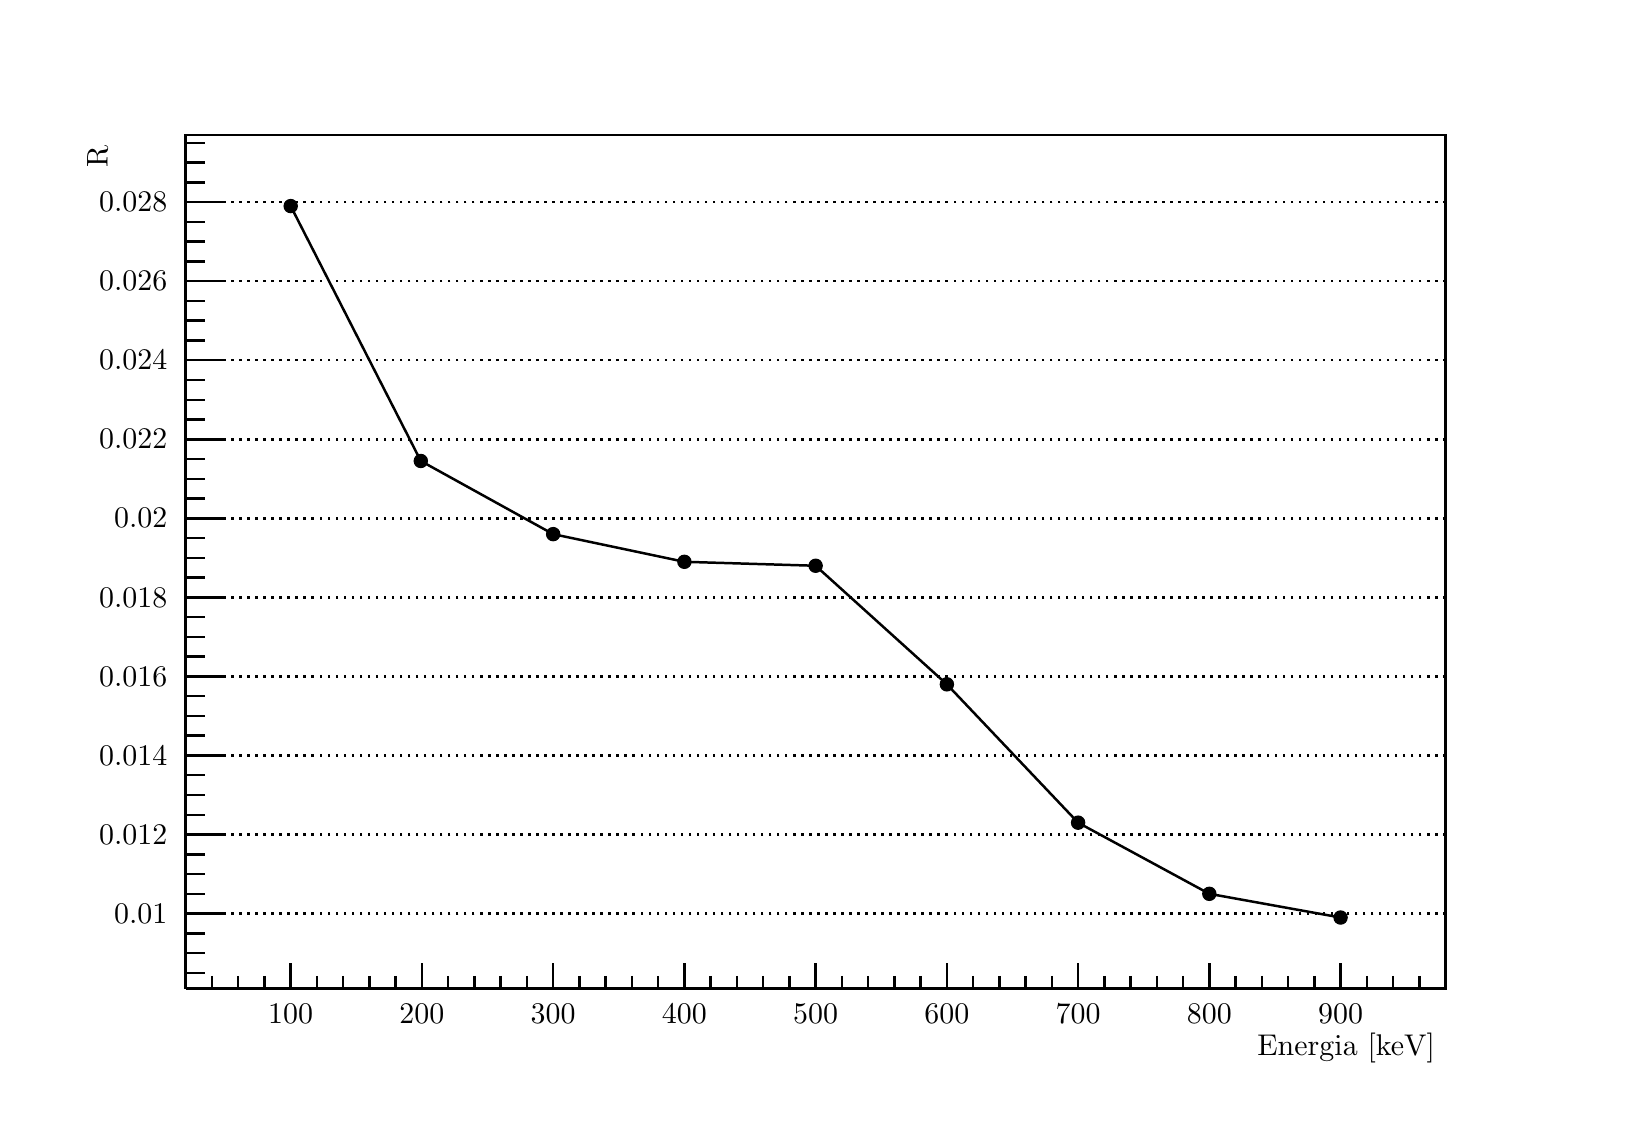
\begin{tikzpicture}
\pgfdeclareplotmark{cross} {
\pgfpathmoveto{\pgfpoint{-0.3\pgfplotmarksize}{\pgfplotmarksize}}
\pgfpathlineto{\pgfpoint{+0.3\pgfplotmarksize}{\pgfplotmarksize}}
\pgfpathlineto{\pgfpoint{+0.3\pgfplotmarksize}{0.3\pgfplotmarksize}}
\pgfpathlineto{\pgfpoint{+1\pgfplotmarksize}{0.3\pgfplotmarksize}}
\pgfpathlineto{\pgfpoint{+1\pgfplotmarksize}{-0.3\pgfplotmarksize}}
\pgfpathlineto{\pgfpoint{+0.3\pgfplotmarksize}{-0.3\pgfplotmarksize}}
\pgfpathlineto{\pgfpoint{+0.3\pgfplotmarksize}{-1.\pgfplotmarksize}}
\pgfpathlineto{\pgfpoint{-0.3\pgfplotmarksize}{-1.\pgfplotmarksize}}
\pgfpathlineto{\pgfpoint{-0.3\pgfplotmarksize}{-0.3\pgfplotmarksize}}
\pgfpathlineto{\pgfpoint{-1.\pgfplotmarksize}{-0.3\pgfplotmarksize}}
\pgfpathlineto{\pgfpoint{-1.\pgfplotmarksize}{0.3\pgfplotmarksize}}
\pgfpathlineto{\pgfpoint{-0.3\pgfplotmarksize}{0.3\pgfplotmarksize}}
\pgfpathclose
\pgfusepathqstroke
}
\pgfdeclareplotmark{cross*} {
\pgfpathmoveto{\pgfpoint{-0.3\pgfplotmarksize}{\pgfplotmarksize}}
\pgfpathlineto{\pgfpoint{+0.3\pgfplotmarksize}{\pgfplotmarksize}}
\pgfpathlineto{\pgfpoint{+0.3\pgfplotmarksize}{0.3\pgfplotmarksize}}
\pgfpathlineto{\pgfpoint{+1\pgfplotmarksize}{0.3\pgfplotmarksize}}
\pgfpathlineto{\pgfpoint{+1\pgfplotmarksize}{-0.3\pgfplotmarksize}}
\pgfpathlineto{\pgfpoint{+0.3\pgfplotmarksize}{-0.3\pgfplotmarksize}}
\pgfpathlineto{\pgfpoint{+0.3\pgfplotmarksize}{-1.\pgfplotmarksize}}
\pgfpathlineto{\pgfpoint{-0.3\pgfplotmarksize}{-1.\pgfplotmarksize}}
\pgfpathlineto{\pgfpoint{-0.3\pgfplotmarksize}{-0.3\pgfplotmarksize}}
\pgfpathlineto{\pgfpoint{-1.\pgfplotmarksize}{-0.3\pgfplotmarksize}}
\pgfpathlineto{\pgfpoint{-1.\pgfplotmarksize}{0.3\pgfplotmarksize}}
\pgfpathlineto{\pgfpoint{-0.3\pgfplotmarksize}{0.3\pgfplotmarksize}}
\pgfpathclose
\pgfusepathqfillstroke
}
\pgfdeclareplotmark{newstar} {
\pgfpathmoveto{\pgfqpoint{0pt}{\pgfplotmarksize}}
\pgfpathlineto{\pgfqpointpolar{44}{0.5\pgfplotmarksize}}
\pgfpathlineto{\pgfqpointpolar{18}{\pgfplotmarksize}}
\pgfpathlineto{\pgfqpointpolar{-20}{0.5\pgfplotmarksize}}
\pgfpathlineto{\pgfqpointpolar{-54}{\pgfplotmarksize}}
\pgfpathlineto{\pgfqpointpolar{-90}{0.5\pgfplotmarksize}}
\pgfpathlineto{\pgfqpointpolar{234}{\pgfplotmarksize}}
\pgfpathlineto{\pgfqpointpolar{198}{0.5\pgfplotmarksize}}
\pgfpathlineto{\pgfqpointpolar{162}{\pgfplotmarksize}}
\pgfpathlineto{\pgfqpointpolar{134}{0.5\pgfplotmarksize}}
\pgfpathclose
\pgfusepathqstroke
}
\pgfdeclareplotmark{newstar*} {
\pgfpathmoveto{\pgfqpoint{0pt}{\pgfplotmarksize}}
\pgfpathlineto{\pgfqpointpolar{44}{0.5\pgfplotmarksize}}
\pgfpathlineto{\pgfqpointpolar{18}{\pgfplotmarksize}}
\pgfpathlineto{\pgfqpointpolar{-20}{0.5\pgfplotmarksize}}
\pgfpathlineto{\pgfqpointpolar{-54}{\pgfplotmarksize}}
\pgfpathlineto{\pgfqpointpolar{-90}{0.5\pgfplotmarksize}}
\pgfpathlineto{\pgfqpointpolar{234}{\pgfplotmarksize}}
\pgfpathlineto{\pgfqpointpolar{198}{0.5\pgfplotmarksize}}
\pgfpathlineto{\pgfqpointpolar{162}{\pgfplotmarksize}}
\pgfpathlineto{\pgfqpointpolar{134}{0.5\pgfplotmarksize}}
\pgfpathclose
\pgfusepathqfillstroke
}
\definecolor{c}{rgb}{1,1,1};
\draw [color=c, fill=c] (0,0) rectangle (20,13.553);
\draw [color=c, fill=c] (2,1.3553) rectangle (18,12.1977);
\definecolor{c}{rgb}{0,0,0};
\draw [c,line width=0.9] (2,1.3553) -- (2,12.1977) -- (18,12.1977) -- (18,1.3553) -- (2,1.3553);
\definecolor{c}{rgb}{1,1,1};
\draw [color=c, fill=c] (2,1.3553) rectangle (18,12.1977);
\definecolor{c}{rgb}{0,0,0};
\draw [c,line width=0.9] (2,1.3553) -- (2,12.1977) -- (18,12.1977) -- (18,1.3553) -- (2,1.3553);
\draw [c,line width=0.9] (2,1.3553) -- (18,1.3553);
\draw [c,line width=0.9] (2,1.3553) -- (2,12.1977);
\draw [c,dotted,line width=0.9] (18,2.30903) -- (2,2.30903);
\draw [c,dotted,line width=0.9] (18,3.31296) -- (2,3.31296);
\draw [c,dotted,line width=0.9] (18,4.31688) -- (2,4.31688);
\draw [c,dotted,line width=0.9] (18,5.32081) -- (2,5.32081);
\draw [c,dotted,line width=0.9] (18,6.32474) -- (2,6.32474);
\draw [c,dotted,line width=0.9] (18,7.32866) -- (2,7.32866);
\draw [c,dotted,line width=0.9] (18,8.33259) -- (2,8.33259);
\draw [c,dotted,line width=0.9] (18,9.33652) -- (2,9.33652);
\draw [c,dotted,line width=0.9] (18,10.3404) -- (2,10.3404);
\draw [c,dotted,line width=0.9] (18,11.3444) -- (2,11.3444);
\draw [c,dotted,line width=0.9] (18,2.30903) -- (2,2.30903);
\draw [c,dotted,line width=0.9] (18,11.3444) -- (2,11.3444);
\draw [c,line width=0.9] (2,1.3553) -- (18,1.3553);
\draw [anchor= east] (18,0.596333) node[scale=1.08185, color=c, rotate=0]{Energia [keV]};
\draw [c,line width=0.9] (3.33333,1.68057) -- (3.33333,1.3553);
\draw [c,line width=0.9] (3.66667,1.51794) -- (3.66667,1.3553);
\draw [c,line width=0.9] (4,1.51794) -- (4,1.3553);
\draw [c,line width=0.9] (4.33333,1.51794) -- (4.33333,1.3553);
\draw [c,line width=0.9] (4.66667,1.51794) -- (4.66667,1.3553);
\draw [c,line width=0.9] (5,1.68057) -- (5,1.3553);
\draw [c,line width=0.9] (5.33333,1.51794) -- (5.33333,1.3553);
\draw [c,line width=0.9] (5.66667,1.51794) -- (5.66667,1.3553);
\draw [c,line width=0.9] (6,1.51794) -- (6,1.3553);
\draw [c,line width=0.9] (6.33333,1.51794) -- (6.33333,1.3553);
\draw [c,line width=0.9] (6.66667,1.68057) -- (6.66667,1.3553);
\draw [c,line width=0.9] (7,1.51794) -- (7,1.3553);
\draw [c,line width=0.9] (7.33333,1.51794) -- (7.33333,1.3553);
\draw [c,line width=0.9] (7.66667,1.51794) -- (7.66667,1.3553);
\draw [c,line width=0.9] (8,1.51794) -- (8,1.3553);
\draw [c,line width=0.9] (8.33333,1.68057) -- (8.33333,1.3553);
\draw [c,line width=0.9] (8.66667,1.51794) -- (8.66667,1.3553);
\draw [c,line width=0.9] (9,1.51794) -- (9,1.3553);
\draw [c,line width=0.9] (9.33333,1.51794) -- (9.33333,1.3553);
\draw [c,line width=0.9] (9.66667,1.51794) -- (9.66667,1.3553);
\draw [c,line width=0.9] (10,1.68057) -- (10,1.3553);
\draw [c,line width=0.9] (10.3333,1.51794) -- (10.3333,1.3553);
\draw [c,line width=0.9] (10.6667,1.51794) -- (10.6667,1.3553);
\draw [c,line width=0.9] (11,1.51794) -- (11,1.3553);
\draw [c,line width=0.9] (11.3333,1.51794) -- (11.3333,1.3553);
\draw [c,line width=0.9] (11.6667,1.68057) -- (11.6667,1.3553);
\draw [c,line width=0.9] (12,1.51794) -- (12,1.3553);
\draw [c,line width=0.9] (12.3333,1.51794) -- (12.3333,1.3553);
\draw [c,line width=0.9] (12.6667,1.51794) -- (12.6667,1.3553);
\draw [c,line width=0.9] (13,1.51794) -- (13,1.3553);
\draw [c,line width=0.9] (13.3333,1.68057) -- (13.3333,1.3553);
\draw [c,line width=0.9] (13.6667,1.51794) -- (13.6667,1.3553);
\draw [c,line width=0.9] (14,1.51794) -- (14,1.3553);
\draw [c,line width=0.9] (14.3333,1.51794) -- (14.3333,1.3553);
\draw [c,line width=0.9] (14.6667,1.51794) -- (14.6667,1.3553);
\draw [c,line width=0.9] (15,1.68057) -- (15,1.3553);
\draw [c,line width=0.9] (15.3333,1.51794) -- (15.3333,1.3553);
\draw [c,line width=0.9] (15.6667,1.51794) -- (15.6667,1.3553);
\draw [c,line width=0.9] (16,1.51794) -- (16,1.3553);
\draw [c,line width=0.9] (16.3333,1.51794) -- (16.3333,1.3553);
\draw [c,line width=0.9] (16.6667,1.68057) -- (16.6667,1.3553);
\draw [c,line width=0.9] (3.33333,1.68057) -- (3.33333,1.3553);
\draw [c,line width=0.9] (3,1.51794) -- (3,1.3553);
\draw [c,line width=0.9] (2.66667,1.51794) -- (2.66667,1.3553);
\draw [c,line width=0.9] (2.33333,1.51794) -- (2.33333,1.3553);
\draw [c,line width=0.9] (2,1.51794) -- (2,1.3553);
\draw [c,line width=0.9] (16.6667,1.68057) -- (16.6667,1.3553);
\draw [c,line width=0.9] (17,1.51794) -- (17,1.3553);
\draw [c,line width=0.9] (17.3333,1.51794) -- (17.3333,1.3553);
\draw [c,line width=0.9] (17.6667,1.51794) -- (17.6667,1.3553);
\draw [c,line width=0.9] (18,1.51794) -- (18,1.3553);
\draw [anchor=base] (3.33333,0.908052) node[scale=1.08185, color=c, rotate=0]{100};
\draw [anchor=base] (5,0.908052) node[scale=1.08185, color=c, rotate=0]{200};
\draw [anchor=base] (6.66667,0.908052) node[scale=1.08185, color=c, rotate=0]{300};
\draw [anchor=base] (8.33333,0.908052) node[scale=1.08185, color=c, rotate=0]{400};
\draw [anchor=base] (10,0.908052) node[scale=1.08185, color=c, rotate=0]{500};
\draw [anchor=base] (11.6667,0.908052) node[scale=1.08185, color=c, rotate=0]{600};
\draw [anchor=base] (13.3333,0.908052) node[scale=1.08185, color=c, rotate=0]{700};
\draw [anchor=base] (15,0.908052) node[scale=1.08185, color=c, rotate=0]{800};
\draw [anchor=base] (16.6667,0.908052) node[scale=1.08185, color=c, rotate=0]{900};
\draw [c,line width=0.9] (2,1.3553) -- (2,12.1977);
\draw [anchor= east] (0.88,12.1977) node[scale=1.08185, color=c, rotate=90]{R};
\draw [c,line width=0.9] (2.48,2.30903) -- (2,2.30903);
\draw [c,line width=0.9] (2.24,2.56001) -- (2,2.56001);
\draw [c,line width=0.9] (2.24,2.81099) -- (2,2.81099);
\draw [c,line width=0.9] (2.24,3.06198) -- (2,3.06198);
\draw [c,line width=0.9] (2.48,3.31296) -- (2,3.31296);
\draw [c,line width=0.9] (2.24,3.56394) -- (2,3.56394);
\draw [c,line width=0.9] (2.24,3.81492) -- (2,3.81492);
\draw [c,line width=0.9] (2.24,4.0659) -- (2,4.0659);
\draw [c,line width=0.9] (2.48,4.31688) -- (2,4.31688);
\draw [c,line width=0.9] (2.24,4.56787) -- (2,4.56787);
\draw [c,line width=0.9] (2.24,4.81885) -- (2,4.81885);
\draw [c,line width=0.9] (2.24,5.06983) -- (2,5.06983);
\draw [c,line width=0.9] (2.48,5.32081) -- (2,5.32081);
\draw [c,line width=0.9] (2.24,5.57179) -- (2,5.57179);
\draw [c,line width=0.9] (2.24,5.82277) -- (2,5.82277);
\draw [c,line width=0.9] (2.24,6.07376) -- (2,6.07376);
\draw [c,line width=0.9] (2.48,6.32474) -- (2,6.32474);
\draw [c,line width=0.9] (2.24,6.57572) -- (2,6.57572);
\draw [c,line width=0.9] (2.24,6.8267) -- (2,6.8267);
\draw [c,line width=0.9] (2.24,7.07768) -- (2,7.07768);
\draw [c,line width=0.9] (2.48,7.32866) -- (2,7.32866);
\draw [c,line width=0.9] (2.24,7.57965) -- (2,7.57965);
\draw [c,line width=0.9] (2.24,7.83063) -- (2,7.83063);
\draw [c,line width=0.9] (2.24,8.08161) -- (2,8.08161);
\draw [c,line width=0.9] (2.48,8.33259) -- (2,8.33259);
\draw [c,line width=0.9] (2.24,8.58357) -- (2,8.58357);
\draw [c,line width=0.9] (2.24,8.83455) -- (2,8.83455);
\draw [c,line width=0.9] (2.24,9.08554) -- (2,9.08554);
\draw [c,line width=0.9] (2.48,9.33652) -- (2,9.33652);
\draw [c,line width=0.9] (2.24,9.5875) -- (2,9.5875);
\draw [c,line width=0.9] (2.24,9.83848) -- (2,9.83848);
\draw [c,line width=0.9] (2.24,10.0895) -- (2,10.0895);
\draw [c,line width=0.9] (2.48,10.3404) -- (2,10.3404);
\draw [c,line width=0.9] (2.24,10.5914) -- (2,10.5914);
\draw [c,line width=0.9] (2.24,10.8424) -- (2,10.8424);
\draw [c,line width=0.9] (2.24,11.0934) -- (2,11.0934);
\draw [c,line width=0.9] (2.48,11.3444) -- (2,11.3444);
\draw [c,line width=0.9] (2.48,2.30903) -- (2,2.30903);
\draw [c,line width=0.9] (2.24,2.05805) -- (2,2.05805);
\draw [c,line width=0.9] (2.24,1.80707) -- (2,1.80707);
\draw [c,line width=0.9] (2.24,1.55609) -- (2,1.55609);
\draw [c,line width=0.9] (2.48,11.3444) -- (2,11.3444);
\draw [c,line width=0.9] (2.24,11.5954) -- (2,11.5954);
\draw [c,line width=0.9] (2.24,11.8463) -- (2,11.8463);
\draw [c,line width=0.9] (2.24,12.0973) -- (2,12.0973);
\draw [anchor= east] (1.9,2.30903) node[scale=1.08185, color=c, rotate=0]{0.01};
\draw [anchor= east] (1.9,3.31296) node[scale=1.08185, color=c, rotate=0]{0.012};
\draw [anchor= east] (1.9,4.31688) node[scale=1.08185, color=c, rotate=0]{0.014};
\draw [anchor= east] (1.9,5.32081) node[scale=1.08185, color=c, rotate=0]{0.016};
\draw [anchor= east] (1.9,6.32474) node[scale=1.08185, color=c, rotate=0]{0.018};
\draw [anchor= east] (1.9,7.32866) node[scale=1.08185, color=c, rotate=0]{0.02};
\draw [anchor= east] (1.9,8.33259) node[scale=1.08185, color=c, rotate=0]{0.022};
\draw [anchor= east] (1.9,9.33652) node[scale=1.08185, color=c, rotate=0]{0.024};
\draw [anchor= east] (1.9,10.3404) node[scale=1.08185, color=c, rotate=0]{0.026};
\draw [anchor= east] (1.9,11.3444) node[scale=1.08185, color=c, rotate=0]{0.028};
\draw [c,line width=0.9] (3.33333,11.2942) -- (4.98567,8.05699) -- (6.66667,7.12788) -- (8.33333,6.7765) -- (10,6.72631) -- (11.6667,5.22042) -- (13.3333,3.46355) -- (15,2.56001) -- (16.6667,2.25884);
\foreach \P in {(3.33333,11.2942), (4.98567,8.05699), (6.66667,7.12788), (8.33333,6.7765), (10,6.72631), (11.6667,5.22042), (13.3333,3.46355), (15,2.56001), (16.6667,2.25884)}{\draw[mark options={color=c,fill=c},mark size=2.402402pt,mark=*] plot
 coordinates {\P};}
\end{tikzpicture}
\\
\begin{tikzpicture}
\pgfdeclareplotmark{cross} {
\pgfpathmoveto{\pgfpoint{-0.3\pgfplotmarksize}{\pgfplotmarksize}}
\pgfpathlineto{\pgfpoint{+0.3\pgfplotmarksize}{\pgfplotmarksize}}
\pgfpathlineto{\pgfpoint{+0.3\pgfplotmarksize}{0.3\pgfplotmarksize}}
\pgfpathlineto{\pgfpoint{+1\pgfplotmarksize}{0.3\pgfplotmarksize}}
\pgfpathlineto{\pgfpoint{+1\pgfplotmarksize}{-0.3\pgfplotmarksize}}
\pgfpathlineto{\pgfpoint{+0.3\pgfplotmarksize}{-0.3\pgfplotmarksize}}
\pgfpathlineto{\pgfpoint{+0.3\pgfplotmarksize}{-1.\pgfplotmarksize}}
\pgfpathlineto{\pgfpoint{-0.3\pgfplotmarksize}{-1.\pgfplotmarksize}}
\pgfpathlineto{\pgfpoint{-0.3\pgfplotmarksize}{-0.3\pgfplotmarksize}}
\pgfpathlineto{\pgfpoint{-1.\pgfplotmarksize}{-0.3\pgfplotmarksize}}
\pgfpathlineto{\pgfpoint{-1.\pgfplotmarksize}{0.3\pgfplotmarksize}}
\pgfpathlineto{\pgfpoint{-0.3\pgfplotmarksize}{0.3\pgfplotmarksize}}
\pgfpathclose
\pgfusepathqstroke
}
\pgfdeclareplotmark{cross*} {
\pgfpathmoveto{\pgfpoint{-0.3\pgfplotmarksize}{\pgfplotmarksize}}
\pgfpathlineto{\pgfpoint{+0.3\pgfplotmarksize}{\pgfplotmarksize}}
\pgfpathlineto{\pgfpoint{+0.3\pgfplotmarksize}{0.3\pgfplotmarksize}}
\pgfpathlineto{\pgfpoint{+1\pgfplotmarksize}{0.3\pgfplotmarksize}}
\pgfpathlineto{\pgfpoint{+1\pgfplotmarksize}{-0.3\pgfplotmarksize}}
\pgfpathlineto{\pgfpoint{+0.3\pgfplotmarksize}{-0.3\pgfplotmarksize}}
\pgfpathlineto{\pgfpoint{+0.3\pgfplotmarksize}{-1.\pgfplotmarksize}}
\pgfpathlineto{\pgfpoint{-0.3\pgfplotmarksize}{-1.\pgfplotmarksize}}
\pgfpathlineto{\pgfpoint{-0.3\pgfplotmarksize}{-0.3\pgfplotmarksize}}
\pgfpathlineto{\pgfpoint{-1.\pgfplotmarksize}{-0.3\pgfplotmarksize}}
\pgfpathlineto{\pgfpoint{-1.\pgfplotmarksize}{0.3\pgfplotmarksize}}
\pgfpathlineto{\pgfpoint{-0.3\pgfplotmarksize}{0.3\pgfplotmarksize}}
\pgfpathclose
\pgfusepathqfillstroke
}
\pgfdeclareplotmark{newstar} {
\pgfpathmoveto{\pgfqpoint{0pt}{\pgfplotmarksize}}
\pgfpathlineto{\pgfqpointpolar{44}{0.5\pgfplotmarksize}}
\pgfpathlineto{\pgfqpointpolar{18}{\pgfplotmarksize}}
\pgfpathlineto{\pgfqpointpolar{-20}{0.5\pgfplotmarksize}}
\pgfpathlineto{\pgfqpointpolar{-54}{\pgfplotmarksize}}
\pgfpathlineto{\pgfqpointpolar{-90}{0.5\pgfplotmarksize}}
\pgfpathlineto{\pgfqpointpolar{234}{\pgfplotmarksize}}
\pgfpathlineto{\pgfqpointpolar{198}{0.5\pgfplotmarksize}}
\pgfpathlineto{\pgfqpointpolar{162}{\pgfplotmarksize}}
\pgfpathlineto{\pgfqpointpolar{134}{0.5\pgfplotmarksize}}
\pgfpathclose
\pgfusepathqstroke
}
\pgfdeclareplotmark{newstar*} {
\pgfpathmoveto{\pgfqpoint{0pt}{\pgfplotmarksize}}
\pgfpathlineto{\pgfqpointpolar{44}{0.5\pgfplotmarksize}}
\pgfpathlineto{\pgfqpointpolar{18}{\pgfplotmarksize}}
\pgfpathlineto{\pgfqpointpolar{-20}{0.5\pgfplotmarksize}}
\pgfpathlineto{\pgfqpointpolar{-54}{\pgfplotmarksize}}
\pgfpathlineto{\pgfqpointpolar{-90}{0.5\pgfplotmarksize}}
\pgfpathlineto{\pgfqpointpolar{234}{\pgfplotmarksize}}
\pgfpathlineto{\pgfqpointpolar{198}{0.5\pgfplotmarksize}}
\pgfpathlineto{\pgfqpointpolar{162}{\pgfplotmarksize}}
\pgfpathlineto{\pgfqpointpolar{134}{0.5\pgfplotmarksize}}
\pgfpathclose
\pgfusepathqfillstroke
}
\definecolor{c}{rgb}{1,1,1};
\draw [color=c, fill=c] (0,0) rectangle (20,13.4957);
\draw [color=c, fill=c] (2,1.34957) rectangle (18,12.1461);
\definecolor{c}{rgb}{0,0,0};
\draw [c,line width=0.9] (2,1.34957) -- (2,12.1461) -- (18,12.1461) -- (18,1.34957) -- (2,1.34957);
\definecolor{c}{rgb}{1,1,1};
\draw [color=c, fill=c] (2,1.34957) rectangle (18,12.1461);
\definecolor{c}{rgb}{0,0,0};
\draw [c,line width=0.9] (2,1.34957) -- (2,12.1461) -- (18,12.1461) -- (18,1.34957) -- (2,1.34957);
\draw [c,line width=0.9] (2,1.34957) -- (18,1.34957);
\draw [anchor= east] (18,0.593811) node[scale=1.01821, color=c, rotate=0]{Energia [keV]};
\draw [c,line width=0.9] (3.33333,1.67347) -- (3.33333,1.34957);
\draw [c,line width=0.9] (3.66667,1.51152) -- (3.66667,1.34957);
\draw [c,line width=0.9] (4,1.51152) -- (4,1.34957);
\draw [c,line width=0.9] (4.33333,1.51152) -- (4.33333,1.34957);
\draw [c,line width=0.9] (4.66667,1.51152) -- (4.66667,1.34957);
\draw [c,line width=0.9] (5,1.67347) -- (5,1.34957);
\draw [c,line width=0.9] (5.33333,1.51152) -- (5.33333,1.34957);
\draw [c,line width=0.9] (5.66667,1.51152) -- (5.66667,1.34957);
\draw [c,line width=0.9] (6,1.51152) -- (6,1.34957);
\draw [c,line width=0.9] (6.33333,1.51152) -- (6.33333,1.34957);
\draw [c,line width=0.9] (6.66667,1.67347) -- (6.66667,1.34957);
\draw [c,line width=0.9] (7,1.51152) -- (7,1.34957);
\draw [c,line width=0.9] (7.33333,1.51152) -- (7.33333,1.34957);
\draw [c,line width=0.9] (7.66667,1.51152) -- (7.66667,1.34957);
\draw [c,line width=0.9] (8,1.51152) -- (8,1.34957);
\draw [c,line width=0.9] (8.33333,1.67347) -- (8.33333,1.34957);
\draw [c,line width=0.9] (8.66667,1.51152) -- (8.66667,1.34957);
\draw [c,line width=0.9] (9,1.51152) -- (9,1.34957);
\draw [c,line width=0.9] (9.33333,1.51152) -- (9.33333,1.34957);
\draw [c,line width=0.9] (9.66667,1.51152) -- (9.66667,1.34957);
\draw [c,line width=0.9] (10,1.67347) -- (10,1.34957);
\draw [c,line width=0.9] (10.3333,1.51152) -- (10.3333,1.34957);
\draw [c,line width=0.9] (10.6667,1.51152) -- (10.6667,1.34957);
\draw [c,line width=0.9] (11,1.51152) -- (11,1.34957);
\draw [c,line width=0.9] (11.3333,1.51152) -- (11.3333,1.34957);
\draw [c,line width=0.9] (11.6667,1.67347) -- (11.6667,1.34957);
\draw [c,line width=0.9] (12,1.51152) -- (12,1.34957);
\draw [c,line width=0.9] (12.3333,1.51152) -- (12.3333,1.34957);
\draw [c,line width=0.9] (12.6667,1.51152) -- (12.6667,1.34957);
\draw [c,line width=0.9] (13,1.51152) -- (13,1.34957);
\draw [c,line width=0.9] (13.3333,1.67347) -- (13.3333,1.34957);
\draw [c,line width=0.9] (13.6667,1.51152) -- (13.6667,1.34957);
\draw [c,line width=0.9] (14,1.51152) -- (14,1.34957);
\draw [c,line width=0.9] (14.3333,1.51152) -- (14.3333,1.34957);
\draw [c,line width=0.9] (14.6667,1.51152) -- (14.6667,1.34957);
\draw [c,line width=0.9] (15,1.67347) -- (15,1.34957);
\draw [c,line width=0.9] (15.3333,1.51152) -- (15.3333,1.34957);
\draw [c,line width=0.9] (15.6667,1.51152) -- (15.6667,1.34957);
\draw [c,line width=0.9] (16,1.51152) -- (16,1.34957);
\draw [c,line width=0.9] (16.3333,1.51152) -- (16.3333,1.34957);
\draw [c,line width=0.9] (16.6667,1.67347) -- (16.6667,1.34957);
\draw [c,line width=0.9] (3.33333,1.67347) -- (3.33333,1.34957);
\draw [c,line width=0.9] (3,1.51152) -- (3,1.34957);
\draw [c,line width=0.9] (2.66667,1.51152) -- (2.66667,1.34957);
\draw [c,line width=0.9] (2.33333,1.51152) -- (2.33333,1.34957);
\draw [c,line width=0.9] (2,1.51152) -- (2,1.34957);
\draw [c,line width=0.9] (16.6667,1.67347) -- (16.6667,1.34957);
\draw [c,line width=0.9] (17,1.51152) -- (17,1.34957);
\draw [c,line width=0.9] (17.3333,1.51152) -- (17.3333,1.34957);
\draw [c,line width=0.9] (17.6667,1.51152) -- (17.6667,1.34957);
\draw [anchor=base] (3.33333,0.904212) node[scale=1.01821, color=c, rotate=0]{100};
\draw [anchor=base] (5,0.904212) node[scale=1.01821, color=c, rotate=0]{200};
\draw [anchor=base] (6.66667,0.904212) node[scale=1.01821, color=c, rotate=0]{300};
\draw [anchor=base] (8.33333,0.904212) node[scale=1.01821, color=c, rotate=0]{400};
\draw [anchor=base] (10,0.904212) node[scale=1.01821, color=c, rotate=0]{500};
\draw [anchor=base] (11.6667,0.904212) node[scale=1.01821, color=c, rotate=0]{600};
\draw [anchor=base] (13.3333,0.904212) node[scale=1.01821, color=c, rotate=0]{700};
\draw [anchor=base] (15,0.904212) node[scale=1.01821, color=c, rotate=0]{800};
\draw [anchor=base] (16.6667,0.904212) node[scale=1.01821, color=c, rotate=0]{900};
\draw [c,line width=0.9] (2,1.34957) -- (2,12.1461);
\draw [anchor= east] (0.88,12.1461) node[scale=1.01821, color=c, rotate=90]{R};
\draw [c,line width=0.9] (2.48,1.81627) -- (2,1.81627);
\draw [c,line width=0.9] (2.24,2.2974) -- (2,2.2974);
\draw [c,line width=0.9] (2.24,2.77853) -- (2,2.77853);
\draw [c,line width=0.9] (2.24,3.25966) -- (2,3.25966);
\draw [c,line width=0.9] (2.24,3.74079) -- (2,3.74079);
\draw [c,line width=0.9] (2.48,4.22192) -- (2,4.22192);
\draw [c,line width=0.9] (2.24,4.70305) -- (2,4.70305);
\draw [c,line width=0.9] (2.24,5.18418) -- (2,5.18418);
\draw [c,line width=0.9] (2.24,5.66531) -- (2,5.66531);
\draw [c,line width=0.9] (2.24,6.14644) -- (2,6.14644);
\draw [c,line width=0.9] (2.48,6.62757) -- (2,6.62757);
\draw [c,line width=0.9] (2.24,7.1087) -- (2,7.1087);
\draw [c,line width=0.9] (2.24,7.58983) -- (2,7.58983);
\draw [c,line width=0.9] (2.24,8.07096) -- (2,8.07096);
\draw [c,line width=0.9] (2.24,8.55209) -- (2,8.55209);
\draw [c,line width=0.9] (2.48,9.03322) -- (2,9.03322);
\draw [c,line width=0.9] (2.24,9.51435) -- (2,9.51435);
\draw [c,line width=0.9] (2.24,9.99548) -- (2,9.99548);
\draw [c,line width=0.9] (2.24,10.4766) -- (2,10.4766);
\draw [c,line width=0.9] (2.24,10.9577) -- (2,10.9577);
\draw [c,line width=0.9] (2.48,11.4389) -- (2,11.4389);
\draw [c,line width=0.9] (2.48,1.81627) -- (2,1.81627);
\draw [c,line width=0.9] (2.48,11.4389) -- (2,11.4389);
\draw [c,line width=0.9] (2.24,11.92) -- (2,11.92);
\draw [anchor= east] (1.9,1.81627) node[scale=1.01821, color=c, rotate=0]{0.015};
\draw [anchor= east] (1.9,4.22192) node[scale=1.01821, color=c, rotate=0]{0.02};
\draw [anchor= east] (1.9,6.62757) node[scale=1.01821, color=c, rotate=0]{0.025};
\draw [anchor= east] (1.9,9.03322) node[scale=1.01821, color=c, rotate=0]{0.03};
\draw [anchor= east] (1.9,11.4389) node[scale=1.01821, color=c, rotate=0]{0.035};
\draw [c,line width=0.9] (3.32378,11.2607) -- (4.98567,6.30372) -- (6.64756,5.15759) -- (8.30946,4.52722) -- (10,4.38395) -- (11.6619,3.69627) -- (13.3238,3.03725) -- (14.9857,2.60745) -- (16.6476,2.26361);
\foreach \P in {(3.32378,11.2607), (4.98567,6.30372), (6.64756,5.15759), (8.30946,4.52722), (10,4.38395), (11.6619,3.69627), (13.3238,3.03725), (14.9857,2.60745), (16.6476,2.26361)}{\draw[mark options={color=c,fill=c},mark size=2.402402pt,mark=*]
 plot coordinates {\P};}
\end{tikzpicture}
\\


